%-------------------------------------------------------------------------------
%                      Template Naskah Skripsi
%               	Berdasarkan format JTETI FT UGM
% 						(c) @gunturdputra 2014
%-------------------------------------------------------------------------------

%Template pembuatan naskah skripsi.
\documentclass{jtetiskripsi}

\renewcommand \thesection{\Alph{section}.}
\renewcommand \thesubsection{\arabic{subsection}.}

%Untuk prefiks pada daftar gambar dan tabel
\usepackage[titles]{tocloft}
\renewcommand\cftfigpresnum{Gambar\  }
\renewcommand\cfttabpresnum{Tabel\   }

%Untuk hyperlink dan table of content
\usepackage[hidelinks]{hyperref}
\newlength{\mylenf}
\settowidth{\mylenf}{\cftfigpresnum}
\setlength{\cftfignumwidth}{\dimexpr\mylenf+2em}
\setlength{\cfttabnumwidth}{\dimexpr\mylenf+2em}

%Untuk Bold Face pada Keterangan Gambar
\usepackage[labelfont=bf]{caption}

%Untuk caption dan subcaption
\usepackage{caption}
\usepackage{subcaption}

\usepackage{enumitem} % <===============================================
\setlist[enumerate]{parsep=0pt}
\newlength{\enumerateparindent} % <=====================================

%pdf
\usepackage{pdfpages}

%table
\usepackage{graphics}

%longtable
\usepackage{longtable}

\usepackage{wrapfig}

%bibliography
\usepackage{natbib}

%equation
\usepackage{amsmath}

%algoritma
\usepackage{algorithm}
\usepackage{algpseudocode}

%listing
\usepackage{listings}
%\usepackage{longtable}
\usepackage{multirow}

%-----------------------------------------------------------------
%Disini awal masukan untuk data proposal skripsi
%-----------------------------------------------------------------
\titleind{Perancangan Aplikasi Pendukung Teknologi Perikanan Modern Berbasis Android}

\fullname{Gian Chiesa Maghriza}

\idnum{1313618021}

%\approvaldate{12 Februari 2019}
%\approvaldate{12 Februari 2019}

\degree{Sarjana Ilmu Komputer}

\yearsubmit{2023}

\program{Ilmu Komputer}

\dept{Ilmu Komputer}

\firstsupervisor{Muhammad Eka Suryana, M. Kom.}
\firstnip{198512232012121002}

\secondsupervisor{Med Irzal, M.Kom.}
\secondnip{197706152003121001}

%-----------------------------------------------------------------
%Disini akhir masukan untuk data proposal skripsi
%-----------------------------------------------------------------

\tolerance=1
\emergencystretch=\maxdimen
\hyphenpenalty=10000
\hbadness=10000

\begin{document}

\cover
%-----------------------------------------------------------------

%-----------------------------------------------------------------
%Disini akhir masukan untuk muka skripsi
%-----------------------------------------------------------------
\chapter*{\centering{\large{LEMBAR PERSETUJUAN HASIL SIDANG SKRIPSI}}}

\begin{figure}[H]
	\centering
	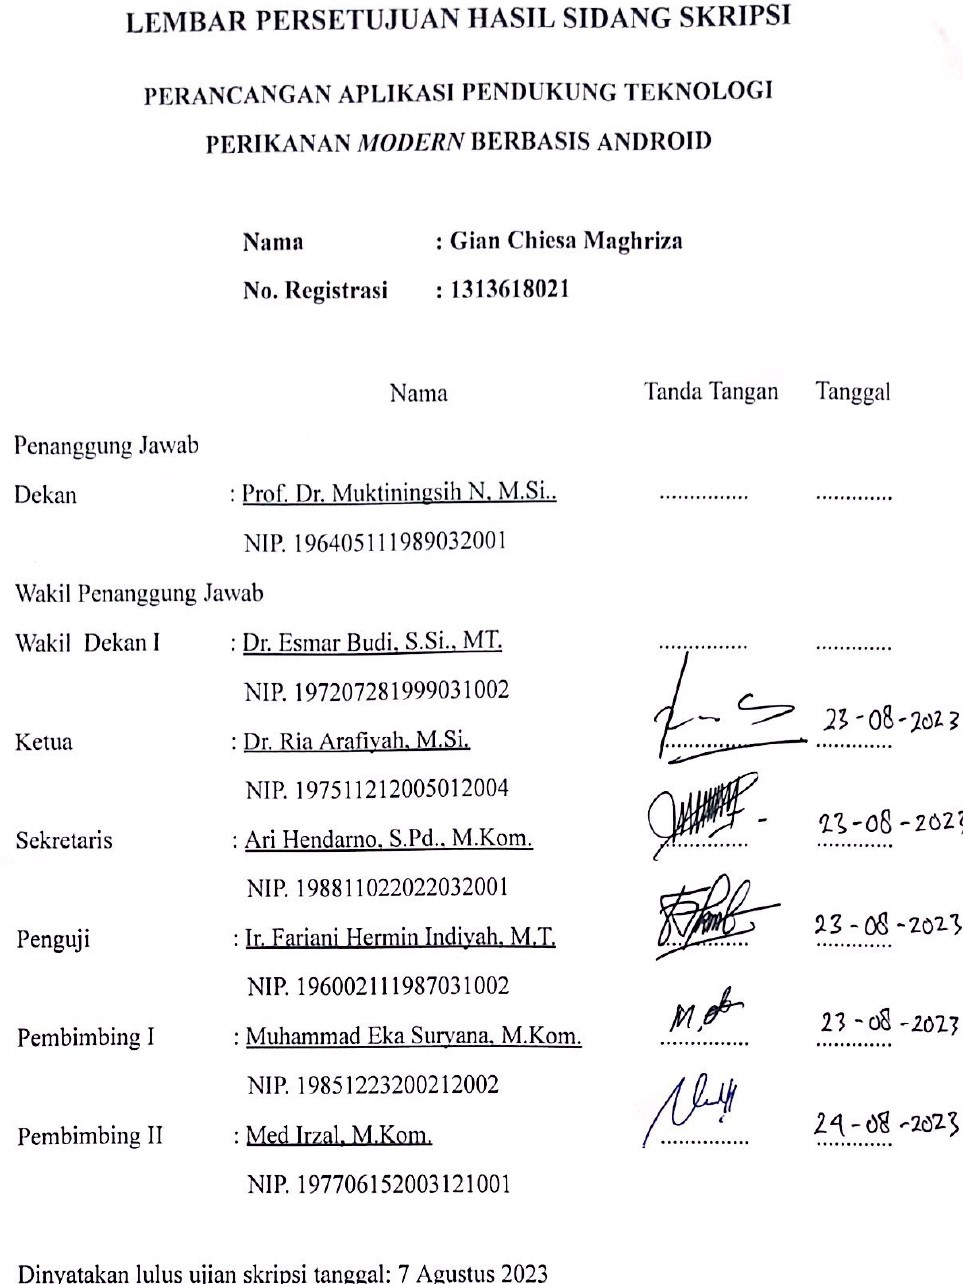
\includegraphics[keepaspectratio,width=0.88\textwidth, height=0.88\textheight]{gambar/lembar-revisi}
\end{figure}
\addcontentsline{toc}{chapter}{LEMBAR PERSETUJUAN HASIL SIDANG}
\chapter*{\centering{\large{LEMBAR PERNYATAAN}}}

Saya menyatakan dengan sesungguhnya bahwa skripsi dengan judull \textbf{"Perancangan Aplikasi Pendukung Teknologi Perikanan Modern Berbasis Android"} yang disusun sebagai syarat untuk memperoleh gelar Sarjana Komputer dari Program Studi Ilmu Komputer Universitas Negeri Jakarta adalah karya ilmiah saya dengan arahan dari dosen pembimbing.

Simber informasi yang diperoleh dari penulis lain yang telah dipublikasikan dan disebutkan dalam teks skripsi ini, telah dicantumkan dalam Daftar Pustaka sesuai dengan norma, kaidah dan etika penulisan ilmiah.

Jika dikemudian hari ditemukan sebagian besar skripsi ini bukan hasil karya saya sendiri dalam bagian tertentu, saya bersedia menerima sanksi pencabutan gelar akdemik yang saya sanding dan sanksi-sanksi lainnya sesuai dengan peraturan dan perundang-undangan yang berlaku.

\vspace{4cm}

\begin{tabular}{p{8,4cm}r}
	&Jakarta, 30 Juli 2023\\
	&\\
	&\\
	&\\
	&Gian Chiesa Maghriza\\
	&1313618021              
\end{tabular}
\addcontentsline{toc}{chapter}{LEMBAR PERNYATAAN}
\chapter*{\centering{\large{HALAMAN PERSEMBAHAN}}}
\null\vfill
\begin{flushright}
\textit{Untuk Keluargaku dan Diriku Sendiri.}
\end{flushright}
\addcontentsline{toc}{chapter}{HALAMAN PERSEMBAHAN}
\chapter*{\centering{\large{ABSTRAK}}}

\begin{spacing}{1}
\textbf{GIAN CHIESA MAGHRIZA}. Perancangan Aplikasi Pendukung Teknologi Perikanan Modern Berbasis Android. Skripsi. Program Studi Ilmu Komputer Fakultas Matematika dan Ilmu Pengetahuan Alam, Universitas Negeri Jakarta. 2023. Di bawah bimbingan Muhammad Eka Suryana, M.Kom dan Med Irzal, M.Kom.
\newline
\newline
Budidaya ikan di perairan tawar merupakan salah satu aspek penting dalam sektor perikanan di Indonesia. Pencatatan data masa budidaya seperti dosis pakan, kematian ikan, grading ikan, dan sortir ikan serta hal yang berkaitan dengan kontrol kolam seperti kondisi air, data kolam merupakan hal penting dalam budidaya ikan. Saat ini pencatatan data-data tersebut masih dilakukan dengan munggunakan kertas sehingga beresiko akan kesalahan dalam perhitungan. Penelitian ini bertujuan untuk membuat aplikasi pendukung teknologi perikanan modern yang membantu pencatatan dalam melakukan aktivitas budidaya perikanan. Jenis Penelitian ini adalah Pengembangan/\textit{Research} and Development. Informasi dan kebutuhan diperoleh dari diskusi yang dilakukan bersama pembudidaya ikan air tawar di \textit{JFT (J Farm Technology)} serta penelusuran literatur melalui membaca berbagai jurnal yang relevan dengan topik penelitian. Diskusi menghasilkan suatu \textit{user requirement} yang menjadi acuan fitur pencatatan yang akan diterapkan pada aplikasi pendukung teknologi perikanan modern. Proses pengembangan sistem ini menggunakan metode \textit{Scrum} dan seluruh aplikasi yang dibuat menggunakan bahasa pemrograman \textit{Dart} dengan \textit{framework flutter}. Hasil akhir dari penelitian ini berupa aplikasi pendukung teknologi perikanan modern yang membantu pembudidaya dalam melakukan pencatatan aktivitas budidaya. Berdasarkan hasil uji coba \textit{User Acceptance Test (UAT)} terdapat 6 fitur yang sudah sesuai dan 4 fitur yang belum sesuai dengan kebutuhan dilapangan, namun 4 fitur tersebut telah diperbaiki sesuai dengan kebutuhan dari pembudidaya ikan air tawar di \textit{JFT (J Farm Technology)}.
\newline
\newline
\noindent \textbf{Kata kunci}: \textit{android, aplikasi, budidaya ikan, teknologi perikanan, scrum, pencatatan}
\end{spacing}
\addcontentsline{toc}{chapter}{ABSTRAK}
\chapter*{\centering{\large{ABSTRACT}}}

\begin{spacing}{1}
\textbf{GIAN CHIESA MAGHRIZA}. Design of a Android Based Application to Support Modern Fisheries Technology. Mini Thesis. Computer Science Department, Faculty of Mathematics and Natural Siences, State University of Jakarta. 2023. Under the guidance Muhammad Eka Suryana, M.Cs dan Med Irzal, M.Cs.
\newline
\newline
\textit{Fish farming in freshwater environments is one of the crucial aspects in the fisheries sector in Indonesia. Recording cultivation data such as feed dosage, fish mortality, fish grading, sorting, and related pond control factors like water conditions and pond data is essential in fish farming. Currently, these data recordings are still done using paper, which poses a risk of errors in calculations. This research aims to develop a supportive application for modern fisheries technology that aids in recording activities within fish farming. This research falls under the category of Research and Development. Information and requirements were obtained through discussions with freshwater fish farmers at JFT (J Farm Technology) and through literature review by studying various journals relevant to the research topic. The discussions resulted in user requirements that serve as a reference for the recording features to be implemented in the modern fisheries technology supportive application. The system development process employs the Scrum methodology, and the entire application is built using the Dart programming language with the Flutter framework. The ultimate outcome of this study is a modern fisheries technology supportive application that assists farmers in recording cultivation activities. Based on the results of the User Acceptance Test (UAT), 6 features were found to be in alignment, while 4 features did not meet field requirements initially. However, these 4 features were subsequently improved to meet the needs of freshwater fish farmers at JFT (J Farm Technology).}
\newline
\newline
\noindent \textbf{Keywordsi}: \textit{android, application, cultivation of fish, fisheries, scrum, recording}
\end{spacing}
\addcontentsline{toc}{chapter}{ABSTRACT}
\chapter*{\centering{\large{KATA PENGANTAR}}}

Puji syukur penulis panjatkan ke hadirat Allah SWT, karena dengan rahmat dan karunia-Nya, penulis dapat menyelesaikan skripsi yang berjudul \textbf{"Perancangan Aplikasi Pendukung Teknologi Perikanan Modern Berbasis Android"}.

Keberhasilan dalam menyusun skripsi ini tidak lepas dari bantuan berbagai pihak yang mana dengan tulus dan ikhlas memberikan masukan guna sempurnanya skripsi ini. Oleh karena itu dalam kesempatan ini, dengan kerendahan hati penulis mengucapkan banyak terima kasih kepada:

\begin{enumerate}

	\item{Yth. Ibu Dr. Ria Arafiyah, M.Si selaku Koordinator Program Studi Ilmu Komputer.}
	\item{Yth. Bapak Muhammad Eka Suryana, M.Kom selaku Dosen Pembimbing I yang telah membimbing, mengarahkan, serta memberikan saran dan koreksi terhadap skripsi ini.}
	\item{Yth. Bapak Med Irzal, M.Kom selaku Dosen Pembimbing II yang telah membimbing, mengarahkan, serta memberikan saran dan koreksi terhadap skripsi ini.}
	\item{Direktur utama PT. Satu Teknologi Digital, bapak Roy Prasetya dan HR PT. Satu Teknologi Digital, bapak Iwan Fauzi yang senantiasa memberikan saya izin untuk dalam memenuhi keperluan skripsi yang sedang saya kerjakan.}
	\item{Pembudidaya dari UD Jfarm yang senantiasa berpartisipasi dalam pembuatan aplikasi dalam skripsi saya.}
	\item{Orang tua penulis yang selama ini telah mendukung dan membantu menyelesaikan skripsi ini.}
	\item{Teman-teman Program Studi Ilmu Komputer 2018 yang telah mendukung dan membantu skripsi ini.}
	\item{Teman-teman dari Kelompok Mahasiswa Peminat Fotografi UNJ yang telah mendukung dan menyemangati saya dalam menyelesaikan skripsi ini.}
	\item{Teman-teman dari mabar Valorant ilmu komputer 2018 yang turut mendukung penulis dalam perngerjaan skripsi penulis.}
	
\end{enumerate}

Penulis menyadari bahwa penyusunan skripsi ini masih jauh dari sempurna karena keterbatasan ilmu dan pengalaman yang dimiliki. Oleh karenanya, kritik dan saran yang bersifat membangun akan penulis terima dengan senang hati. Akhir kata, penulis berharap tugas akhir ini bermanfaat bagi semua pihak khususnya penulis sendiri. Semoga Allah SWT senantiasa membalas kebaikan semua pihak yang telah membantu penulis dalam menyelesaikan skripsi ini.

\vspace{4cm}

\begin{tabular}{p{8,4cm}r}
	&Jakarta, 30 Juli 2023\\
	&\\
	&\\
	&\\
	&Gian Chiesa Maghriza
\end{tabular}
\addcontentsline{toc}{chapter}{KATA PENGANTAR}
\tableofcontents 
\addcontentsline{toc}{chapter}{DAFTAR ISI}
\listoffigures
\addcontentsline{toc}{chapter}{DAFTAR GAMBAR}
\listoftables
\addcontentsline{toc}{chapter}{DAFTAR TABEL}

\begin{counterpage}
\end{counterpage}
%Disini awal masukan untuk Bab
%-----------------------------------------------------------------
%!TEX root = ./template-skripsi.tex
%-------------------------------------------------------------------------------
% 								BAB I
% 							LATAR BELAKANG
%-------------------------------------------------------------------------------

\chapter{PENDAHULUAN}

\section{Latar Belakang Masalah}

Indonesia memiliki dua sumber perikanan, yaitu tangkap laut dan budidaya ikan air tawar. Berbeda dengan tangkap laut yang hanya membutuhkan skil dan modal perkapalan, budidaya ikan air tawar relatif memerlukan permodalan yang lebih besar untuk dilakukan seperti  lahan,  infrastruktur tambak/kolam, dan juga pakan. Belum lagi budidaya ikan yang tidak mudah dan memerlukan keterampilan khusus. Namun demikian bukan berarti ikan hasil tangkap menguasai sepenuhnya pasar perikanan mengingat beberapa pertimbangan yakni citarasa ikan air tawar dan air laut berbeda, ikan air tawar yang dapat diperjualbelikan dalam keadaaan hidup, biaya dan waktu transportasi tidak memadai untuk menjangkau daerah pegunungan guna mengirim ikan hasil tangkapan. Dengan modal yang besar, tentunya hal tersebut juga diikuti oleh nilai ekonomi yang berpotensi.

\begin{figure}[H]
	\centering
	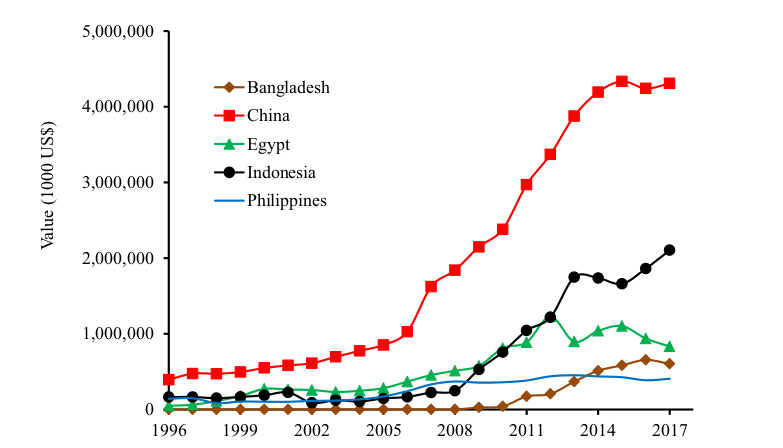
\includegraphics[keepaspectratio, width=12cm]{gambar/produksi_nila}
	\caption{Produksi \emph{Tilapia} 1996-2017 (Fattah, 2020)}
	\label{gambar:produksi_nila}
\end{figure}

Diantara jenis ikan air tawar yang memiliki nilai ekonomi, Lele dan Nila adalah jenis ikan yang memiliki masa panen yang cenderung singkat. Masing-masing memiliki masa panen 3 bulan serta 5 bulan. Ikan Nila (\textit{Tilapia}) memegang 8 persen dari total produksi ikan dunia dengan produksi meningkat dari tahun ke tahun \citep{fattah2020}, hal tersebut dapat dilihat pada gambar 1.1. Sementara itu data KKP menunjukkan, volume produksi \textit{Tilapia} di pulau jawa juga memiliki tren yang sama. Kecuali DKI Jakarta yang stagnant dan Jawa Barat yang menurun, seperti yang ditunjukan oleh gambar 1.2. DKI Jakarta tidak memiliki lahan pertanian yang tidak luas sehingga dapat dimaklumi, untuk Jawa Barat penyebab penurunnya masih perlu dihuhungkan dengan ekspor-impor \textit{Tilapia}, dan jumlah pertumbuhan rumah tangga perikanan \citep{kkp2022}. Ditinjau dari gambar 1.3, indeks konsumsi ikan di Jawa Barat trendnya mengalami peningkatan sehingga logika yang wajar dari turunnya jumlah produksi ikan di Jawa Barat adalah tidak terupdatenya data.

\begin{figure}[H]
	\centering
	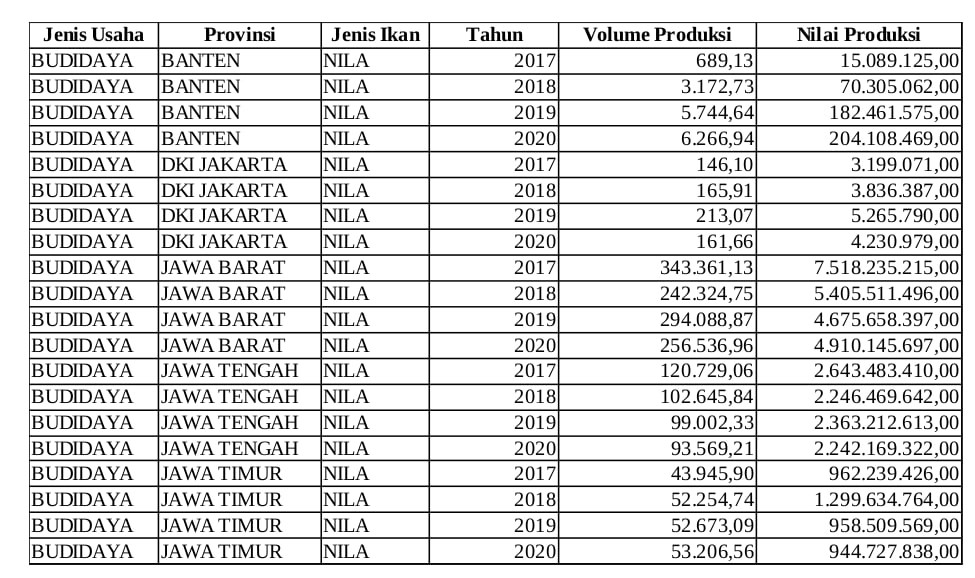
\includegraphics[keepaspectratio, width=13cm]{gambar/produksi_tilapia_jawa}
	\caption{Produksi \emph{Tilapia} Di Pulau Jawa (KKP, 2021)}
	\label{gambar:produksi_tilapia_jawa}
\end{figure}
\begin{figure}[H]
	\centering
	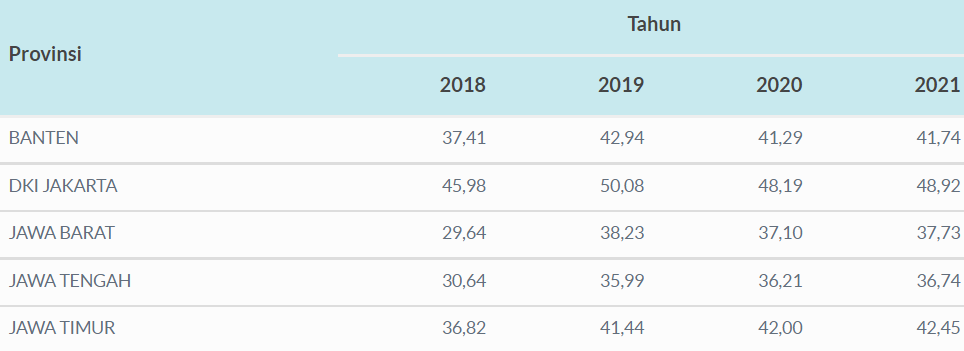
\includegraphics[keepaspectratio, width=12cm]{gambar/indeks_konsumsi_ikan2}
	\caption{Indeks Konsumsi Ikan Di Pulau Jawa (KKP, 2022)}
	\label{gambar:indeks_konsumsi_ikan2}
\end{figure}

Budidaya ikan air tawar di Indonesia secara umum terbagi menjadi 3 kelas yaitu \textit{extensive}, \textit{Semi-Intensive} dan \textit{Intensive}. Budidaya ekstensif adalah budidaya yang dilakukan dengan alami tanpa ada penambahan pakan buatan dari kata tradisional atau ekstensif seharusnya kita mengerti apa itu tradisional. Sementara untuk intensif dan semi-intensif, perbedaan dari keduanya terdapat pada kemampuan tebar padat ikan, dimana \textit{Intensive aquaculture system} mampu mengakomodasi kepadatan ikan dengan luas penampang lahan yang sama. \textit{Semi Intensive} salah satu contohnya pada sistem Tambak. Sementara \textit{Intensive system} diwakili oleh \textit{Biofloc Technology (BFT)} dan \textit{Recirculating Aquaculture System (RAS)}. Ditinjau dari tingkat keahlian yang dibutuhkan \textit{BFT} memerlukan tenaga ahli khusus. 

Kualitas air yang dihasilkan pada \textit{BFT} di atas kualitas air biasa terutama dalam 2 hal yakni, kekayaan dari bahan organik dalam air, dan kemamuan air dalam mereduksi \textit{toxic} secara alami. \textit{BFT} mendapatkan hal tersebut dengan bantuan \textit{Microbacteria} dari keluarga \textit{Bacillus sp} \citep{fattah2020}. \textit{RAS} memiliki kelebihan yaitu tidak dibutuhankan teknisi khusus kecuali saat instalasi kolam. Namun, \textit{RAS} memiliki kemampuan tebar padat yang lebih rendah dibanding \textit{BFT} sehingga skala produktivitasnya masih lebih rendah dibanding sistem \textit{BFT}. Sistem \textit{BFT} memiliki kemampuan tebar padat yang tinggi seperti yang di tunjukan pada gambar 1.4. Namun demikian \textit{BFT} memiliki kelemahan utama yaitu butuh tenaga ahli yang mumpuni atau rumah tangga yang mengaplikasikan \textit{BFT} akan mengalami kegagalan. Dari data peningkatan produksi ikan hasil budidaya ikan air tawar yang telah penulis sebutkan diatas, maka penulis tertarik untuk melakukan penelitian terkait budidaya ikan air tawar untuk membantu pembudidaya dalam melakukan kegiatannya.

\begin{figure}[H]
	\centering
	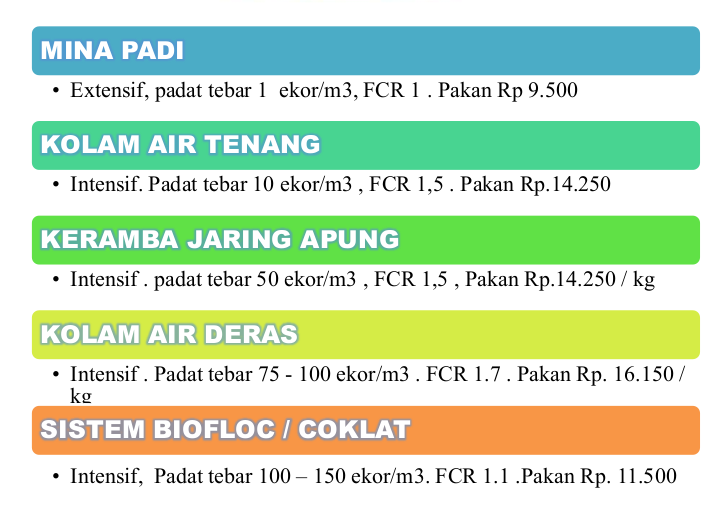
\includegraphics[keepaspectratio, width=9cm]{gambar/tebar_padat}
	\caption{Perbandingan Tebar Padat Kolam \citep{setiawan2021}}
	\label{gambar:tebar_padat}
\end{figure}

Dalam penelitian ini, penulis telah melakukan wawancara dengan UD Jfam sebagai salah satu lembaga budidaya yang bergerak di bidang budidaya ikan air tawar modern berbasis \textit{BFT} yang beralamat di desa Pamagersari, kecamatan Jasinga, Kabupaten Bogor yang menjadi narasumber. Narasumber mengungkapkan permasalahan yang dihadapi selama proses budiddaya di antarnya tenaga ahli bidang \textit{BFT} di UD Jfarm melakukan pemeriksaan kualitas air yang ketat setiap hari. Pengukuran kualitas air ini dilakukan untuk setiap kolam budidaya yang ada seperti yang ditunjukkan pada Gambar 1.5. Hal ini tentunya berimplikasi pada pengelolaan arsip formulir tersebut perlu dilakukan dengan benar dan rapi agar data yang dikumpulkan dapat dievaluasi sebagai dasar pertimbangan \textit{treatment} yang akan dilakukan pada suatu kolam budidaya. Jika hal ini tidak dilakukan, maka berpotensi pada kegagalan proses budidaya berbasis \textit{BFT}. Potensi kegagalan tersebut juga diperbesar dengan metode pencatatan yang dilakukan masih berbasis kertas. Atas dasar masalah tersebut, penulis mengusulkan pengembangan aplikasi pendukung teknologi perikanan modern yang dapat membantu pembudidaya ikan air tawar, dalam hal ini UD Jfam melakukan pencatatan data yang dibutuhkan selama musim budidaya berlangsung.

\begin{figure}[H]
	\centering
	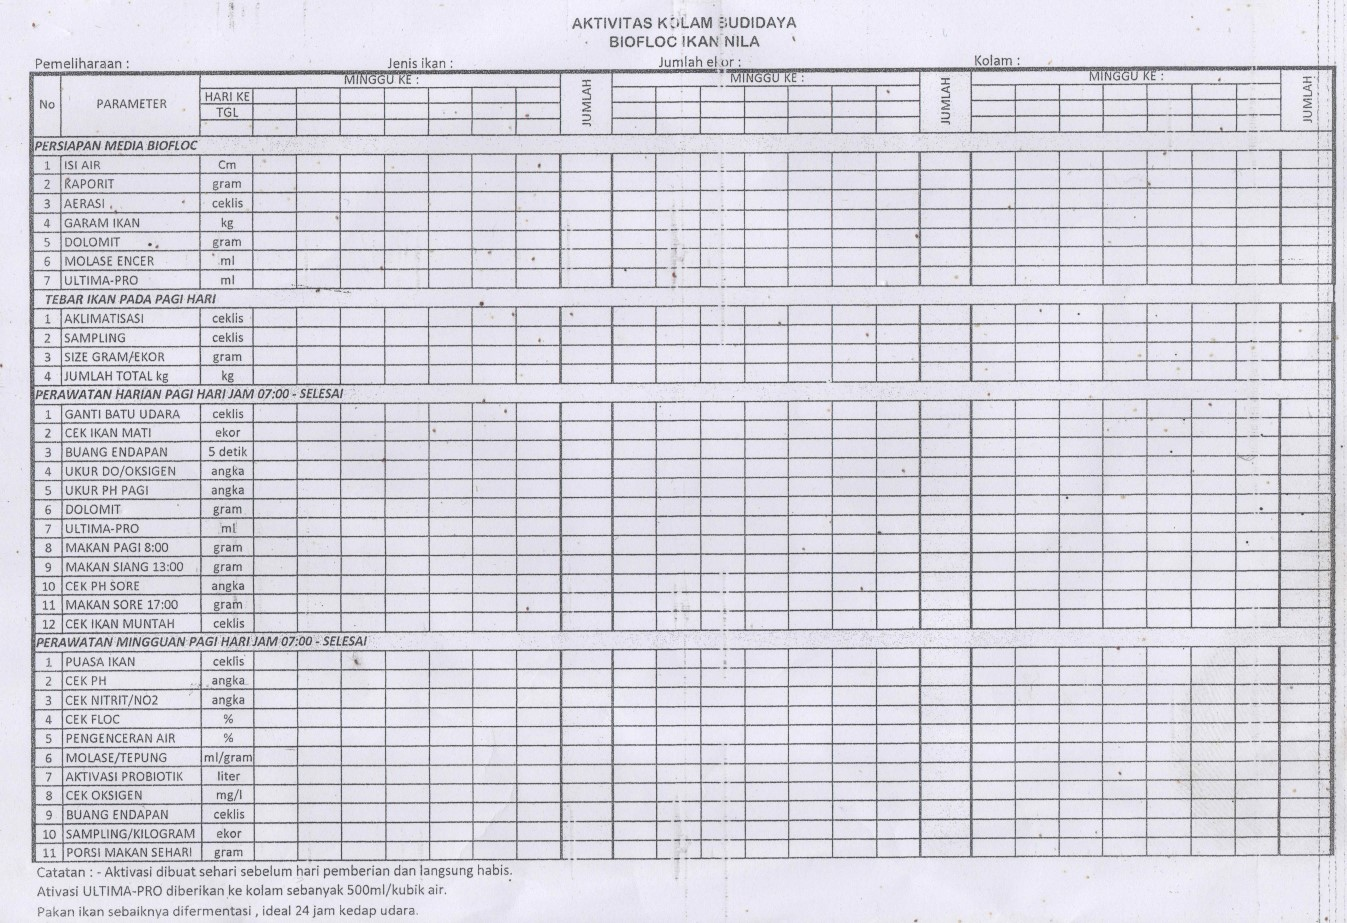
\includegraphics[keepaspectratio, width=14cm]{gambar/form_pencatatan_manual}
	\caption{Form Pencatatan Kualitas Air}
	\label{gambar:form_pencatatan_manual}
\end{figure}

Sudah banyak peneliti di Indonesia  yang berkontribusi dalam berbagai teknologi \textit{Aqua Culture}. \citep{supriati2018} meneliti dan mengembangkan Sistem Informasi Akuntansi Budidaya Perikanan berbasis \textit{SAK EMKM} dan \textit{Android}. Aplikasi yang dikembangkan diperuntukkan untuk Kelompok Tani yang tersusun atas Ketua, Sekretaris, Bendahara, dan Seksi Sarana Produksi perikanan. Aplikasi ini memfasilitasi sejumlah fitur seperti transaksi jual-beli, kas keluar-masuk, dan pembukuan. Penelitian yang sejenis dilakukan oleh \citep{widhiastika2021}, aplikasi hasil penelitian memfasilitasi user untuk melakukan transaksi jual beli perikanan. Aplikasi yang dibuat dinamakan dengan FO-KLIK. Dikembangkan dengan \textit{Android} yang dipasangkan dengan \textit{Firebase}. Selain transaksi jual beli, FO-Klik turut menyediakan fasilitas diskusi dan informasi nilai gizi dari suatu produk item perikanan. Namun tidak dilengkapi dengan manajemen keuangan seperti yang dilakukan oleh \citep{supriati2018}. Selain dari penelitian diatas, perancangan aplikasi terkait budidaya ikan air tawar juga dapat dilakukan berdasarkan metode atau sistem budidaya yang digunakan. Adapun skripsi Andri Rahmanto yang berjudul "Perancangan Arsitektur Aplikasi Budidaya Perikanan Modern pada \textit{Backend} yang Bertanggung Jawab Melayani Transaksi \textit{Query Webservice} Dengan Menggunakan Teknologi \textit{Flask Microservice}" dimana penulis akan menggunakan \textit{Backend} yang telah buat dalam bentuk \textit{REST API}.

Berdasarkan latar belakang yang telah dijelaskan, Peneliti mengusulkan pengembangan aplikasi manajemen budidaya perikanan. Aplikasi ini berpotensi meningkatkan jumlah ikan yang dipanen dan menurunkan angka kematian sehingga mampu menurunkan harga jual ikan dengan adanya stok melimpah. Dengan demikian, dapat terwujud ketahanan pangan wilayah. Aplikasi ini diharapkan dapat membantu petani meningkatkan efisiensi dari setiap masa budidaya yang dijalani.

\section{Rumusan Masalah}
Dari uraian latar belakang di atas, perumusan masalah pada penelitian ini ialah “Bagaimana perancangan aplikasi pendukung teknologi perikanan modern berbasis android?”

\section{Pembatasan Masalah}
Pembatasan masalah pada penelitian ini yaitu:
\begin{enumerate}
	\item Aplikasi pendukung teknologi perikanan modern dikembangkan sampai pada fitur pencatatan dan manajemen masa budidaya.
		
	\item Penelitian ini hanya merangcang bagian \textit{frontend} dari aplikasi pendukung teknologi perikanan modern	 			
\end{enumerate}

\section{Tujuan Penelitian}

 Membuat aplikasi pendukung teknologi perkanan modern yang memudahkan pencatatan data budidaya perikanan.

\section{Manfaat Penelitian}
\begin{enumerate}
	\item Bagi penulis
		
	Memperluas pengetahuan tentang teknologi perikanan modern, menambah pengalaman dalam \textit{programming}, memperoleh gelar sarjana di bidang Ilmu Komputer, serta menjadi media untuk penulis dalam mengaplikasikan ilmu yang didapatkan dari kampus.
		
	\item Bagi Program Studi Ilmu Komputer
	 	
	Penelitian ini dapat menjadi pembuka untuk penelitian di masa depan, dan dapat memberikan panduan bagi mahasiswa program studi Ilmu Komputer tentang perancangan aplikasi teknologi perikanan modern.
	
	\item Bagi Universitas Negeri Jakarta
	 	
	Menjadi evaluasi akademik program studi Ilmu Komputer dalam penyusunan skripsi sehingga dapat meningkatkan kualitas pendidikan dan lulusan program studi Ilmu Komputer di Universitas Negeri Jakarta.
	 			
\end{enumerate}


% Baris ini digunakan untuk membantu dalam melakukan sitasi
% Karena diapit dengan comment, maka baris ini akan diabaikan
% oleh compiler LaTeX.
\begin{comment}
\bibliography{daftar-pustaka}
\end{comment}

 %!TEX root = ./template-skripsi.tex
%-------------------------------------------------------------------------------
%                            BAB II
%               KAJIAN TEORI
%-------------------------------------------------------------------------------

\chapter{KAJIAN PUSTAKA} 

\section{Konsep Budidaya Ikan Air Tawar}

Budidaya adalah kegiatan  memproduksi dan mengembangkan biota (organisme) dalam lingkungan yang terkendali untuk mendapatkan keuntungan. Budidaya ikan air tawar merupakan kegiatan yang dilakukan untuk meningkatkan produktivitas perairan,  khususnya ikan air tawar. Kegiatan budidaya dimaksudkan untuk memperbanyak, menumbuhkan dan meningkatkan kualitas biota perairan itu sendiri untuk menghasilkan keuntungan. Sementara budidaya perikanan modern merupakan metode budidaya yang menggabungkan teknologi terbaru dan ilmu pengetahuan untuk menciptakan lingkungan yang optimal bagi pertumbuhan dan kesehatan ikan \citep{bangkit2016}.

Akuakultur (budidaya ikan) merupakan salah satu subsektor yang diharapkan dapat mewujudkan misi mensejahterakan perikanan. Akuakultur tingkat rendah berkontribusi pada kesejahteraan petani ikan untuk menjamin ketersediaan pangan, gizi dan kesehatan di daerah. Budidaya perikanan modern menggunakan pelet dan konsetrat sebagai sumber pakan, selain itu juga diterapkan berbagai treatment kedalam sistem budidaya untuk membantu proses budidaya ikan. Contoh metode budidaya perikanan modern yaitu RAS dan Biofloc.  


\section{\textit{Food Conversion Ratio (FCR)}}
FCR (Feed Conversion Ratio) pada budidaya ikan adalah suatu ukuran yang menyatakan rasio jumlah pakan yang dibutuhkan untuk menghasilkan 1 kg daging ikan. FCR juga sering digunakan untuk mengetahui kualitas pakan yang diberikan terhadap pertumbuhan ikan. Informasi mengenai FCR ikan yang dibudidayakan sangat penting karena berkaitan dengan efisiensi pakan dan efisiensi musim budidaya. Menurut \citep{effendie1997} FCR ikan didapatkan melalui rumus berikut.

\begin{equation*}
	FCR=\frac{Berat Total Ikan Panen(Kg)}{Jumlah Pakan(Kg)}
\end{equation*}

Informasi mengenai FCR ikan yang dibudidayakan sangat penting karena berkaitan dengan efisiensi pakan. Efisiensi pakan berfungsi mengukur tingkat penggunaan input, yakni pakan dan output berupa bobot daging ikan. Semakin kecil nilai efisiensi pakan, berarti pakan yang diberikan sudah baik. Efisiensi pakan berhubungan dengan pertambahan berat, konsumsi pakan, dan konversi pakan. Pertambahan berat dapat dihitung dengan mengurangi bobot badan ikan saat panen dengan bobot ikan pada awal penebaran.

Sementara itu, konversi pakan merupakan pembagian antara berat badan yang dicapai pada bulan berlangsung dengan konsumsi pakan pada bulan tersebut. Konversi pakan didapatkan dengan membagi total pakan yang dikonsumsi dengan total hasil produksi.

Efisiensi berkaitan erat dengan biaya yang harus Anda keluarkan selama budidaya. Apabila efisiensi pakan tidak bagus, kemungkinan besar biaya pakan yang dikeluarkan juga besar. Padahal, pakan merupakan komponen penting dan besar dalam usaha budidaya. Semakin besar biaya pakan, akan semakin besar juga biaya produksi yang dibutuhkan.

\section{\emph{Recirculating aquaculture system (RAS)}}

RAS merupakan sistem budidaya yang menggunakan air daur ulang yang pertama kali diperkenalkan di Amerika Serikat pada awal tahun 1960 dan mulai diterapkan sejak tahun 1990-an. Teknologi RAS pada saat itu menjadi solusi atas permasalahan pencemaran organik sungai dari tempat budidaya bersamaan dengan permintaan benih ikan salmon yang tinggi yang dibutuhkan sepanjang waktu (kontinu). Kualitas suatu perairan merupakan syarat penting yang dapat mempengaruhi kelangsungan hidup perkembangan, pertumbuhan, dan tingkat produksi ikan. Lingkungan yang baik sangat diperlukan untuk kelangsungan hidup organisme akuatik. Sistem ini telah banyak dikembangkan dan iterapkan dibeberapa negara maju, seperti Amerika, Israel, Singapura, German serta Norwegia selama kurun waktu 20-30 tahun ini \citep{fadhil2010}.

Teknologi RAS menawarkan sebuah alternatif teknologi budidaya melalui perbaikan kualitas air dan penggunaan kembali (re-use). Penggunaan RAS secara intensif terbukti dapat mengurangi secara signifikan konsumsi air dan konsentrasi nutrien melalui perbaikan dan pengembangan teknologi secara berkelanjutan \citep{thesiana2015}. RAS dapat digunakan untuk mengontrol beberapa parameter kualitas air penting seperti oksigen terlarut, karbondioksida, amonia, nitrit, nitrat, pH, salinitas, dan padatan tersuspensi. Hal ini memungkinkan terciptanya kondisi pemeliharaan yang baik untuk pertumbuhan dan pemanfaatan pakan yang lebih optimal \citep{dalsgaard2013}.

\section{\emph{Biofloc Technology}}

Teknologi bioflok merupakan teknologi penggunaan bakteri baik heterotrof maupun autotrof yang dapat mengonversi limbah organik secara intensif menjadi kumpulan mikroorganisme yang berbentuk flok, kemudian dapat dimanfaatkan oleh ikan sebagai sumber makanan. Di dalam flok terdapat beberapa organisme pembentuk seperti bakteri, plankton, jamur, alga, dan partikel tersuspensi yang memengaruhi struktur dan kandungan nutrisi bioflok, namun komunitas bakteri merupakan mikroorganisme paling dominan dalam pembentukan flok dalam bioflok. 

Agregat bioflok memiliki rentang ukuran partikel yang luas, mulai dari yang mikroskopis hingga yang lebih besar dari 1 mm. Bahkan organisme yang lebih besar seperti copepoda dan nematoda dapat memakan flok dan menjadi bagian yang tidak terpisahkan dari beberapa agregat. Kepadatan flok dengan berat basah biasanya hanya sedikit lebih besar dari 1 g/mL, jadi agregat akan tenggelam perlahan-lahan dan relatif mudah dipelihara suspensinya. Dengan porositas hingga 99 persen (ruang kosong), nutrisi, oksigen, dan produk limbah mudah dipertukarkan di antara bagian dalam flok dan air di sekitarnya, dan ini ditingkatkan oleh pencampuran umum dalam sistem bioflok\citep{samocha2019}.

Mikroorganisme bioflok bervariasi antar sistem dan juga dalam sistem yang sama dari waktu ke waktu mengidentifikasi fluktuasi dalam komposisi taksonomi bakteri, mikroalga, ragi, dan mikroorganisme lain dalam flok dari sistem bioflok ikan nila. Di antara bakteri dan ragi taksa adalah Aeromonas spp., Vibrio spp., Enterobac ter sp., Nitrospira sp., Bacillus spp., Sphingomonas sp., Pseudomonas spp., Microthrix sp., Nitrobacter sp., Micrococcus sp., Alcaligenes sp., dan Rhodotorula sp. Bakteri biasanya mendominasi bioflok di sistem akuakultur. Tidak hanya berlimpah (hingga 100 juta bakteri/mL), tetapi juga menunjukkan keragaman yang tinggi. terdapat gambaran menyeluruh pembahasan banyak faktor yang menentukan komposisi flok, diantaranya adalah suhu, salinitas, pH, penyinaran, intensitas pencampuran vertikal, dan jenis karbon organik yang tersedia untuk metabolisme bakteri.

Laju perkembangan flok bisa ditingkatkan dengan cara menambahkan organik karbon untuk merangsang pembentukan flok. Perkembangan dipengaruhi oleh berbagai faktor, yang terutama adalah suhu, oksigen terlarut, pH, beban organik, cahaya, dan pencampuran. \citep{samocha2019} juga menjelaskan mengenai faktor-faktor tersebut:

\begin{enumerate}
	\item Agregat lebih besar dan lebih padat di tempat yang suhunya lebih tinggi dan oksigen terlarut lebih tinggi.
	\item Pencampuran yang intens mengganggu agregat dan mengurangi ukuran flok rata-rata.
	\item Laju pemompaan tinggi melalui lubang kecil mengurangi ukuran flok.
	\item Oksigen terlarut lebih rendah mendukung filamen bakteri, kemungkinan karena rasio permukaan-ke-volume yang tinggi.
	\item pH mempengaruhi flok secara langsung, setiap spesies memiliki range pH opminal masing masing dan berhubungan langsung dengan alkalinitas, karbon anorganik, dan amonia.
	\item Muatan organik tinggi berpromosi lebih cepat berkembang.
	\item Cahaya mempengaruhi kelimpahan organisme fotoautotrofik (yaitu, cyanobacteria, ganggang hijau, diatom, dinoflagellata, rhodophyta, dll.) dalam flok.
\end{enumerate}

Di antara keunggulan bioflok dalam akuakultur adalah nilai nutrisinya yang tinggi, perannya dalam meningkatkan kualitas air, dan efek probiotiknya pada ikan:
\begin{enumerate}
	\item Bioflok sebagai pakan

	Bioflok memiliki kualitas nutrisi yang mirip dengan makanan yang dimakan ikan liar di habitat alaminya. Mempertahankan kepadatan flok yang sesuai di seluruh siklus tanaman dapat mengurangi kebutuhan akan pakan yang diformulasikan \citep{avnimelech2009} yang biasanya menyumbang setidaknya setengah dari biaya produksi dalam akuakultur tradisional. Kuantitas dan kualitas bahan organik disimpan oleh bakteri akhirnya menentukan nilai gizi flok. Bahan organik yang disimpan ini tergantung pada jumlah dan jenis organik karbon yang tersedia untuk pertumbuhan bakteri. intinya adalah bahwa "bioflok adalah apa yang dimakannya". Jika substrat organik yang tepat disediakan, kemudian floc akan menyimpan senyawa berkualitas tinggi itu, maka hal tersebut akan berkontribusi terhadap kebutuhan nutrisi ikan.

	\item Bioflok dan kualitas air

	Di luar nilai nutrisinya, bakteri bioflok dapat dikelola untuk meningkatkan kualitas air. Ini dapat diklasifikasikan menurut caranya memperoleh yaitu, autotrof dan heterotrof. Baik organisme autotrofik dan heterotrofik yang mengisi agregat bioflok meningkatkan kualitas air dengan asimilasi atau transformasi senyawa nitrogen anorganik terlarut (amonia, nitrit, nitrat) yang berbeda derajat, hal ini berbahaya bagi ikan. Untuk tujuan ini, sistem yang didominasi bioflok dapat dikelola mendukung bakteri autotrofik, bakteri heterotrofik, atau kombinasi keduanya dalam sistem mixotrophic. Setiap pilihan memiliki perbedaan implikasi terhadap kualitas air.

	\item Bioflok dan respon immune

	Beberapa jenis ikan memiliki sistem kekebalan yang labil. Ini berarti bahwa mereka tidak memiliki antibodi-antigen spesifik mekanisme untuk menanggapi patogen baru. Populasi mikroba dalam sistem bioflok, Namun, mungkin berperan dalam mengaktifkan sistem kekebalan non spesifik mereka, menghasilkan pertahanan
\end{enumerate}

Pada sistem akuakultur dengan teknologi bioflok, air media kultur hanya sekali dimasukkan dalam wadah, dan digunakkan sampai panen. Penambahan air hanya untuk pengganti penguapan dan pengontrolan kepadatan bioflok \citep{avnimelech2009}. Dibanding sistem resirkulasi yang sangat kompleks, sistem kultur dengan teknologi bioflok hanya menggunakan satu wadah, yakni wadah kultur. Penguraian bahan organik oleh bakteri dan mikroorganisme pengurai, sampai pada pemanfaatan hasil penguraian oleh mikroalga dan mikroorganisme yang tumbuh, terjadi dalam wadah secara seimbang dengan kepadatan organisme kultur yang sangat tinggi. Pengontrolan kualitas air terjadi dalam wadah kultur itu sendiri, oleh sistem bioflok yang sudah berjalan dalam wadah kultur. Sistem ini sangat murah, sederhana ramah lingkungan dan memiliki produktifitas yang sangat tinggi \citep{taw2012}.

\section{Front-end dan Back-End}

Frontend adalah bagian yang dilihat dan dilihat oleh pengguna untuk berinteraksi dengannya, seperti menu, formulir kontak, dll. Dalam konteks web, front end dibuat dengan menggunakan HyperText Markup Language (HTTP), Cascading Style Sheets (CSS), dan juga JavaScript. Sehingga, suatu URL bisa bekerja dan menampilkan situs website dengan baik. Sementara dalam aplikasi mobile, front end dibuat dengan menggunakan widget untuk menampilkan suatu fitur untuk berkomunikasi dengan pengguna. Oleh karena itu, front end juga bisa disebut sebgai client-side.

Di sisi lain, backend biasanya terdiri dari tiga bagian: server, aplikasi, dan DB. Bagian belakang teknologi biasanya terdiri dari bahasa seperti PHP, Ruby, Python, dll. Pada bagian back end, semua hal yang dibuat di dalam front end ataupun sistem dan server dibalik dibuatnya situs website atau aplikasi bisa bekerja sebagaimana mestinya. Mereka juga sering disebut dengan server-side.

\section{Dart}

Bahasa pemrograman Dart merupakan bahasa pemrograman general-purpose yang dirancang oleh Lars Bak dan Kasper Lund. Bahasa pemrograman ini dikembangkan sebagai bahasa pemrograman aplikasi yang dapat dengan mudah untuk dipelajari dan disebarkan. Bahasa pemrograman Dart dapat digunakan secara bebas oleh para developer, karena bahasa ini dirilis secara open-source oleh Google di bawah lisensi BSD. Bahasa pemrograman Dart merupakan bahasa pemrograman berbasis class dan berorientasi terhadap obyek dengan menggunakan sintaks bahasa pemrograman \citep{kelvin2021}. Berikut adalah contoh program sederahana dari Dart guna lebih memahami bahasa pemrograman tersebut:

\begin{enumerate}
	\item \textit{Main Function}

	Setiap aplikasi mempunyai Main Fuction, berikut adalah contoh Main Function yang akan menampilkan teks pada console. Untuk menerapkannya, bisa digunakan print() function.
	
	\begin{figure}[H]
		\centering
		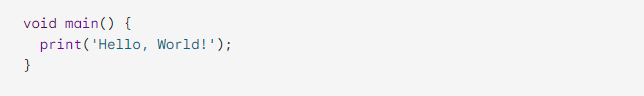
\includegraphics[keepaspectratio, width=12cm]{gambar/helloworld}
		\caption{Contoh Main Function}
		\label{gambar:main}
	\end{figure}
	
	\item Deklarasi \textit{Variables}

	Berikut adalah contoh deklarasi Variable pada dart:
	\begin{figure}[H]
		\centering
		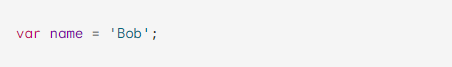
\includegraphics[keepaspectratio, width=12cm]{gambar/implisitvar}
		\caption{Contoh Deklarasi Variable}
		\label{gambar:deklarasivariable}
	\end{figure}
	Pada gambar 2.2 dapat diketahui bahwa terdapat variable yang bernama name dengan bentuk String bernilai "Bob". Variable akan disimpulkan secara implisit dalam bentuk String meskiput tidak dideklarasi secara eksplisit, namun jika dibutuhkan untuk mendeklarasikan variabel secara eksplisit, maka menggunakan cara deklarasi secara eksplisit seperti pada gambar 2.3.
	\begin{figure}[H]
		\centering
		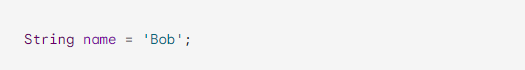
\includegraphics[keepaspectratio, width=12cm]{gambar/eksplisitvar}
		\caption{Contoh Deklarasi Variabel Secara Eksplisi}
		\label{gambar:deklarasivariableeksplisit}
	\end{figure}
	
	\item\textit{Classes}

	Dart adalah bahasa berorientasi objek dengan Class dan pewarisan berbasis mixin. Setiap objek adalah turunan dari Class, dan semua Class kecuali Null turun dari Objek. Pewarisan berbasis mixin berarti meskipun setiap Class (kecuali Top-Class) memiliki tepat satu superclass, Class dapat digunakan kembali dalam beberapa hierarki Class. Metode Extendsi adalah cara untuk menambahkan fungsionalitas ke Class tanpa mengubah Class atau membuat subclass. Dapat Dilihat pada gambar 2.4 yaitu contoh sebuah Class pada bahasa pemrogramman Dart.
	\begin{figure}[H]
		\centering
		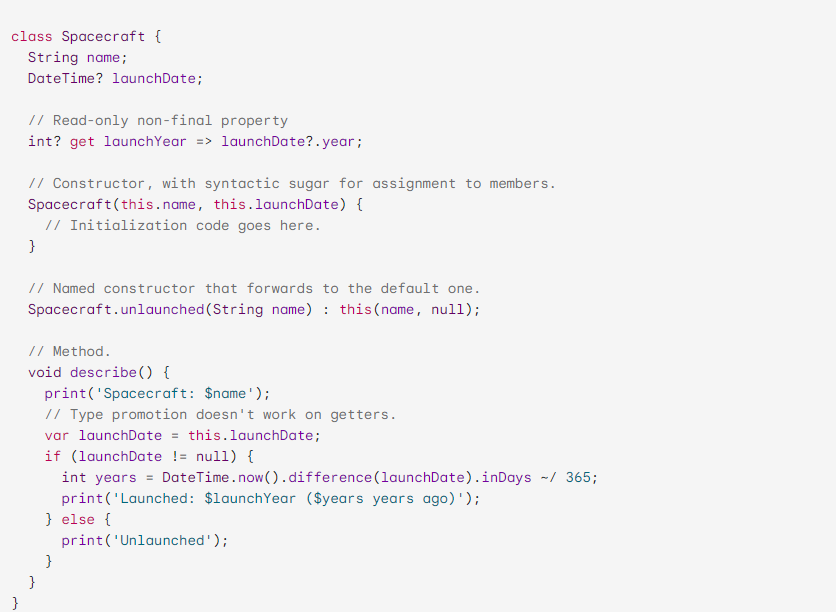
\includegraphics[keepaspectratio, width=9cm]{gambar/Classes}
		\caption{Contoh Class Pada Dart}
		\label{gambar:Class}
	\end{figure}

\end{enumerate}


\section{Flutter}

Flutter telah diresmikan sejak tahun 2015 oleh developer Dart yaitu Sky. Eric Seidel (Direktur untuk Flutter diGoogle). Flutter adalah cross-platform framework yang dibuat oleh Google untuk membangun berbagai aplikasi seperti android mobile, iOS mobile, web, dan desktop. sedangkan menurut \citep{napoli2019} Flutter adalah kerangka antarmuka pengguna portabel (UI) Google untuk membangun aplikasi modern, asli, dan reaktif untuk iOS dan Android. Framework ini menggunakan widgets untuk membuat UI dan Dart sebagai bahasa pemograman untuk mengembangkan aplikasinya. Widget dapat diibaratkan dengan permainan Lego yang bisa menambahkan berbagai macam jenis bongkahan plastik kecil dan mengubah tampilan UI sesuai dengan yang diinginkan oleh developer.

Flutter mempunyai dua macam widget untuk pengembang aplikasi pakai, yaitu Material Design dan Cupertino. Material Design adalah bahasa design yang dibuat oleh Google, design ini sama dengan design yang dipakai pada Android. Cupertino atau dengan sebutan lain gaya iOS adalah bahasa design yang dipakai oleh iOS. Flutter mempunyai lebih banyak widget Material Design daripada widget Cupertino, walaupun demikian, pada OS perangkat yang berbeda, widget bisa dipakai secara cross platform. Flutter memiliki berbagai macam keuntungan dibanding framework lain diantaranya:


\begin{enumerate}
	\item Tingkatkan produktivitas

	Dalam mengembangkan aplikasi berbasis Android dan iOS, Anda hanya membutuhkan satu basis kode. Ini membuat Anda lebih menghemat waktu dan tim.
	
	\item Tingkatkan produktivitas

	Tampilan desain yang sangat bagus. Flutter menyediakan widget cantik yang dapat disesuaikan dengan mudah untuk membuat aplikasi terlihat lebih menarik. Jadi, dengan menggunakan Flutter, developer dari setiap level keahlian akan lebih mudah membuat aplikasi terlihat lebih baik.

	\item Mudah untuk dipelajari

	Flutter adalah framework yang mudah dipelajari. Selain itu, Flutter juga memungkinkan developer aplikasi untuk membangun aplikasi tanpa menggunakan banyak kode seperti pada framework lainnya.

	\item Performa kerangka kerja yang hebat

	\item Pembuatan hemat biaya

	Membuat dua aplikasi (Android dan iOS) dengan menggunakan satu codebase tentunya dapat lebih menghemat biaya pengembangan aplikasi.

	\item Tersedia dalam berbagai pilihan aplikasi IDE (Integrated Development Environment)

	Anda dapat memilih untuk mengembangkan aplikasi (Flutter) menggunakan Android Studio, atau dengan VS Code.

	\item Dokumentasi lengkap dan komunitas aktif.

	Anda dapat membuka dokumentasi melalui situs resmi Flutter. Selain itu, Anda juga bisa bergabung dengan komunitas untuk berdiskusi dengan sesama pengguna Flutter.

\end{enumerate}


\section{Flutter Widget}

Flutter menggunakan konsep widget untuk membuat tampilannya. Widget adalah komponen UI yang membangun aplikasi Flutter. Setiap membuat UI dalam Flutter akan menciptakan berbagai macam pohon widgets . Berikut beberapa informasi mengenai widget:
\begin{enumerate}
	\item Widget digunakan untuk membuat UI, seperti: baris, kolom, stack, card, form, dan padding.
	\item Pada Widget, developer dapat melakukan styling, seperti: tipe font, ukuran, berat, warna, batas, dan bayangan. 
	\item Widget dapat berupa kumpulan bentuk dan formulir.
\end{enumerate}

Diantara widget-widget tersebut, ada beberapa widget yang sering digunakan dan diterapkan dalam berbagai macam aplikasi seperti: CardView, PageView, Bottom Navigation View. Untuk mengetahui lebih lanjut tentang wdget-widget pada flutter.

\section{Metode Scrum}
Metode Scrum diciptakan oleh Jeff Sutherland dan tim pengembangnya pada awal 1990-an. Sutherland, Viktorov, Blount dan Puntikov menggambarkan Scrum sebagai “Proses pengembangan perangkat lunak \textit{Agile} yang dirancang untuk menambah energi, fokus, kejelasan, dan transparansi bagi tim proyek yang mengembangkan sistem perangkat lunak” \citep{sutherland2007}. Proses Scrum mematuhi prinsip-prinsip pendekatan \textit{Agile}. Prinsip pendekatan \textit{Agile} berfokus pada memuaskan pelanggan melalui pengiriman awal perangkat lunak yang berharga; membolehkan perubahan kebutuhan; kolaborasi antara pengembang dan pelaku bisnis; perangkat lunak yang berfungsi (sebagai ukuran kemajuan); menjaga desain tetap sederhana; dan secara berkala, membuat tim merenungkan bagaimana menjadi lebih efektif selama proses pengembangan.

Scrum menawarkan cara yang dapat disesuaikan untuk bekerja pada proyek yang berbeda yang memiliki berbagai persyaratan dan Scrum memiliki keunggulan seperti pemilihan persyaratan atau spesifikasi kebutuhan yang fleksibel untuk \textit{sprint} dan tidak ada prosedur khusus yang harus diikuti. Prinsipnya adalah bekerja secara iteratif hingga mencapai waktu yang ditentukan dan dapat memenuhi kebutuhan konsumen. Scrum menerapkan metode ilmiah empirisme. Scrum 
menggantikan pendekatan algoritmik terprogram dengan pendekatan heuristik, dengan menghormati orang dan pengaturan diri untuk menghadapi ketidakpastian dan memecahkan masalah yang kompleks. Unit dasar Scrum adalah tim kecil dari beberapa orang. Tim Scrum terdiri dari satu Scrum Master yang bertanggung jawab untuk membangun Scrum sebagaimana didefinisikan dalam Panduan Scrum, satu Product Owner yang bertanggung jawab untuk memaksimalkan nilai produk yang dihasilkan dari pekerjaan Tim Scrum, dan Developers yang berkomitmen untuk menciptakan aspek apa pun dari Increment yang dapat digunakan setiap Sprint. Dalam Tim Scrum, tidak ada sub-tim atau hierarki. Ini adalah unit profesional yang kohesif yang berfokus pada satu tujuan pada satu waktu, Sasaran Produk. Aktivitas-aktivitas yang ditentukan digunakan di Scrum agar terciptanya keteraturan dan meminimalkan kebutuhan akan rapat yang tidak ditentukan dalam Scrum. Semua aktivitas dibatasi oleh waktu. Setelah Sprint dimulai, durasinya tetap dan tidak dapat dipersingkat atau diperpanjang. Aktivitas yang tersisa dapat berakhir setiap kali tujuan aktivitas tercapai, memastikan jumlah waktu yang tepat dihabiskan tanpa membiarkan pemborosan dalam proses. Aktivitas-aktivitas yang terdapat pada Scrum adalah Sprint, Sprint Planning, Daily Scrum, Sprint Review, Sprint Retrospective.

Penjelasan lebih lanjut mengenai Scrum dapat dilihat pada jurnal \citep{sutherland2020} yang berjudul "Scrum Guides". Adapun penelitian Andri Rahmanto menggunakan metode scrum dalam pengembangan penelitiannya yang berjudul "Perancangan Arsitektur Aplikasi Budidaya Perikanan Modern pada Backend yang Bertanggung Jawab Melayani Transaksi Query Webservice Dengan Menggunakan Teknologi Flask Microservice". 

\section{\textit{Unit Testing}}
Unit testing merupakan salah satu tipe pengujian perangkat lunak dimana setiap fungsi atau komponen dari perangkat lunak diuji. Tujuan dari unit testing adalah untuk memastikan fungsi pada perangkat lunak sudah berjalan sesuai dengan ekspetasi (Hamilton, 2022). Menurut Rosa dan Shalahuddin (2013: 277), “Unit testing berfokus pada pengujian unit terkecil (komponen perangkat lunak atau modul) dari desain perangkat lunak. Semua fungsi pada perangkat lunak diuji untuk memastikan bahwa input dan output unit sesuai dengan yang diinginkan”.

Pressman (2012) menyebutkan bahwa teknik yang dilakukan pada unit testing adalah “berfokus pada setiap unit perangkat lunak (misalnya komponen, kelas, atau objek konten dari aplikasi atau web) seperti yang diterapkan dalam kode program”. Kode program dikaji apakah terdapat kesalahan. Kesalahan pada kode program dapat diidentifikasi dengan menggunakan White-Box Testing. Sedangkan menurut Rosa dan Shalahuddin (2013), “White-Box Testing (pengujian kotak putih) merupakan pengujian perangkat lunak atau aplikasi dari segi desain dan kode program untuk mengetahui apakah perangkat lunak mampu menghasilkan fungsi-fungsi, masukan, dan keluaran yang sesuai dengan spesifikasi.

Proses unit testing memastikan fungsi-fungsi pada aplikasi yang telah dikembangkan peneliti memenuhi persyaratan, dapat berjalan dengan baik, dan memiliki input serta output sesuai yang diinginkan. Berdasarkan definisi di atas dapat disimpulkan bahwa unit testing merupakan salah satu tipe pengujian fungsi atau unit pada perangkat lunak untuk memastikan apakah perangkat lunak mampu untuk menghasilkan input dan output sesuai dengan spesifikasi yang telah ditentukan.

\section{\textit{User Acceptance Test (UAT)}}
Menurut Perry, William E, (2006) User Acceptance Test (UAT) yaitu pengujian untuk verifikasi apakah fungsi pada sistem telah berjalan dengan kebutuhan, pengujian dilakukan oleh user dimana user tersebut adalah staff/karyawan perusahaan yang langsung berinteraksi dengan sistem. Menurut Black, acceptance testing pada umumnya menunjukkan bahwa sistem telah memenuhi persyaratan-persyaratan tertentu. Pada pengembangan software dan hardware komersial, acceptance test biasanya disebut juga "alpha tests" (yang dilakukan oleh pengguna in-house) dan "beta tests" (yang dilakukan oleh pengguna yang sedang menggunakan atau akan menggunakan sistem tersebut).

Hady, Haryono, Rahayu, (2019) menyebutkan bahwa pelaksanaan UAT terdapat pada akhir proses pengujian saat sistem siap digunakan. Tujuan utama UAT adalah untuk memvalidasi apakah sistem diterima atau ditolak, memenuhi spesifikasi sistem, dan mengembangkan perangkat lunak yang mampu memenuhi kebutuhan user. Proses UAT memastikan bahwa aplikasi pendukung teknologi perikanan modern, sudah layak diujikan secara masif, memenuhi harapan pengguna, dan bekerja seperti yang diharapkan. Dari definisi yang telah dipaparkan dapat disimpulkan bahwa UAT adalah pengujian pada akhir proses yang dilakukan oleh pengguna pada sebuah sistem untuk memastikan fungsi-fungsi yang terdapat pada sistem tersebut telah berjalan dengan baik dan sesuai dengan kebutuhan pengguna
%!TEX root = ./template-skripsi.tex
%-------------------------------------------------------------------------------
%                            BAB III
%               			PEMBAHASAN
%-------------------------------------------------------------------------------

\chapter{METODOLOGI PENELITIAN}

\section{Deskripsi Penelitian}

Aplikasi yang akan dibuat pada penelitian ini adalah aplikasi pendukung teknologi perikanan modern. Aplikasi berfungsi untuk mencatat setiap kegiatan yang dilakukan oleh petani ikan air tawar selama masa budidaya berlangsung. Selain hal tersebut, aplikasi ini juga dapat mengukur \textit{Food Conversion Ratio} dari setiap musim budidaya yang diselesaikan oleh petani. 

\section{Desain Penelitian}

\begin{figure}[H]
	\centering
	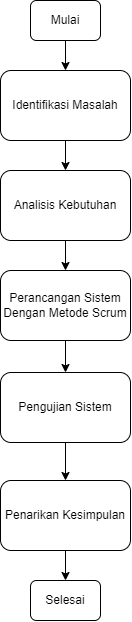
\includegraphics[keepaspectratio, width=2cm]{gambar/tahapan}
	\caption{Tahapan Penelitian}
	\label{gambar:tahapan}
\end{figure}

Agar penelitian berjalan lebih terstruktur dan mudah, maka penulis memerlukan desain penelitian. Desan penelitian merupakan proses dan tahapan yang dilakukan penulis dalam melakukan pembuatan aplikasi pendukung teknologi perikanan modern dengan metode scrum. 
Tahapan penelitian yang akan dilaksanakan penulis dalam perancangan aplikasi dapat dilihat pada gambar \ref{gambar:tahapan}.

\section{Analisis Kebutuhan}

Berdasarkan uraian pada lampiran A yang berisi tentang wawancara analisis kebutuhan fitur untuk aplikasi, prioritas fitur pada aplikasi pendukung teknologi perikanan modern akan berfokus pada penerapan dari backend yang telah dibuat oleh Andri Rahmanto kedalam aplikasi. Berikut adalah \textit{usecase} yang telah didefinisikan berdasarkan hasil wawancara.

\begin{figure}[H]
	\centering
	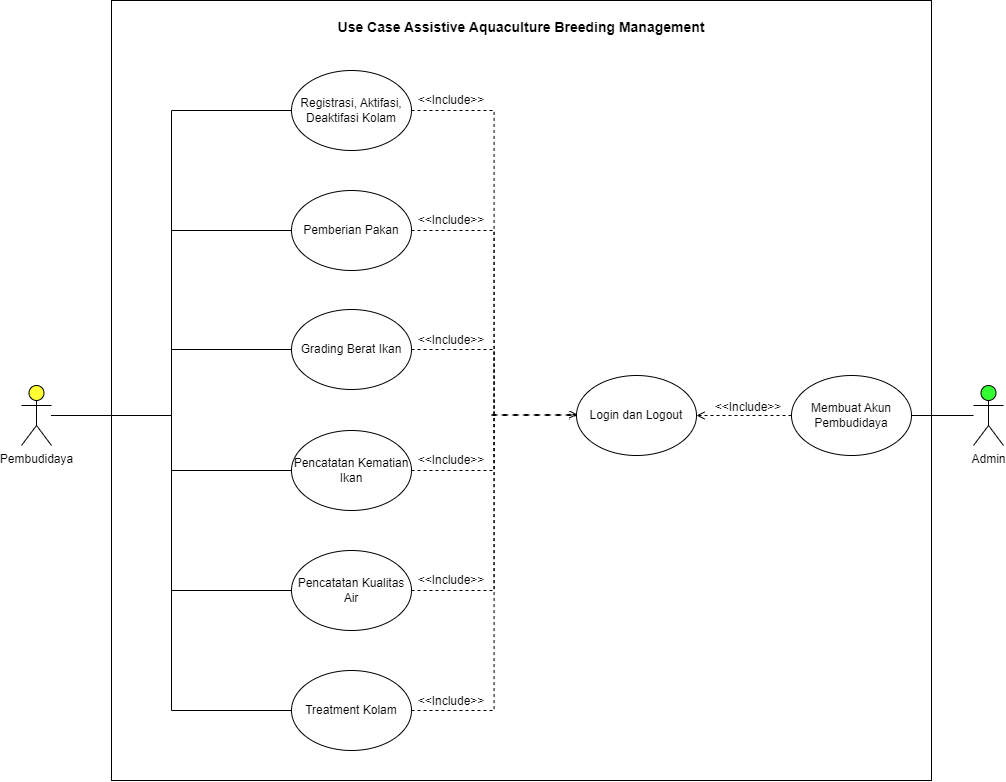
\includegraphics[keepaspectratio, width=13cm]{gambar/usecaseaquabreeding2}
	\caption{Use Case}
	\label{gambar:usecase}
\end{figure}

\section{Perancangan Sistem}

Metode perancangan sistem pada penelitian ini sesuai dengan komponen yang ada di dalam metode Scrum. Komponen-komponen tersebut terdiri dari \textit{product backlog}, \textit{sprint backlog}, \textit{sprint}, \textit{daily scrum}, dan \textit{pengujian sistem}. Aktivitas-aktivitas yang ditentukan digunakan di Scrum agar terciptanya keteraturan. Semua aktivitas dibatasi oleh waktu. Setelah Sprint dimulai, durasinya tetap dan tidak dapat dipersingkat atau diperpanjang. Aktivitas yang tersisa dapat berakhir setiap kali tujuan aktivitas tercapai, memastikan jumlah waktu yang tepat dihabiskan tanpa membiarkan pemborosan dalam proses. Aktivitas-aktivitas yang terdapat pada Scrum adalah Sprint, Sprint Planning, Daily Scrum, Sprint Review, Sprint Retrospective. tahapan dan aktivitas tersebut dapat dilihat pada gambar \ref{gambar:scrumflow}. 

\begin{figure}[H]
	\centering
	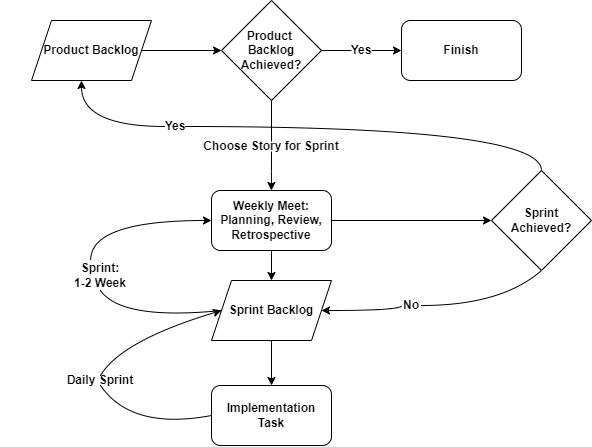
\includegraphics[keepaspectratio, width=11cm]{gambar/scrumflow}
	\caption{Tahapan dan aktivitas yang dilakukan dalam metode scrum}
	\label{gambar:scrumflow}
\end{figure}

\begin{enumerate}
\setlength{\enumerateparindent}{2em}
	\item{\textit{Product Backlog}}
	
	\hspace{\enumerateparindent} Tabel 3.1 merupakan tabel \textit{product backlog} aplikasi pendukung teknologi perikanan modern yang telah dibuat berdasarkan diskusi dengan \textit{Scrum Master}. Setiap \textit{item} dari \textit{product backlog} ini akan diimplementasikan pada \textit{sprint} dari awal hingga selesai.

\begin{table}[H]
	\caption{\textit{Product Backlog}}
	\label{product_backlog}
	\begin{tabular}{@{} |p{0.5cm}|p{8cm}|p{1.5cm}|p{2.5cm}| @{}}
		\hline
		\textbf{No} & \textbf{\textit{Story}} & \textbf{\textit{Sprint}} & \textbf{\textit{Status}} \\
		\hline
		1 & Membuat halaman dasboard & 1 & \\
		\hline
		2 & Membuat fitur registrasi kolam dan aktifasi Musim budidaya & 2 dan 3 & \\
		\hline
		3 & Membuat fitur pemberian pakan & 3 & \\
		\hline
		4 & Membuat fitur grading berat ikan perkolam & 4 & \\
		\hline
		5 & Membuat fitur pencatatan kematian & 5 & \\
		\hline
		6 & Membuat fitur treatmet kolam & 6 dan 7 & \\
		\hline
		7 & Membuat fitur pencatatan kualitas air harian &  8  & \\
		\hline
		8 & Membuat fitur pencatatan kualitas air mingguan & 9 & \\
		\hline
		9 & Membuat fitur perpindahan ikan antar kolam & 10 & \\
		\hline
		10 & Membuat fitur Multi User & 11 & \\
		\hline
	\end{tabular}
\end{table}

	\hspace{\enumerateparindent} Berdasarkan tabel \ref{product_backlog}, \textit{Product Backlog} pada penelitian ini terdiri dari 3 komponen, yaitu \textit{story}, \textit{sprint}, \textit{status}. \textit{Story} merupakan task besar yang nantinya akan dipecah lagi menjadi \textit{task-task} yang kecil di dalam \textit{Sprint}. Komponen \textit{sprint} pada tabel ini menandakan pada \textit{sprint} berapa \textit{story} tersebut akan dilaksanakan. Komponen \textit{status} menjelaskan apakah \textit{story} tersebut sudah selesai atau belum.

	\item{\textit{Sprint Backlog}}

	\hspace{\enumerateparindent} \textit{Sprint backlog} adalah daftar task yang perlu dikerjakan ataupun yang sudah dikerjakan pada \textit{sprint}. Di dalam \textit{sprint backlog}, berbagai \textit{task} kecil dibuat. Dengan Sprint Backlog, seluruh anggota tim dapat melihat perkembangan dari setiap pekerjaan.

	\item{\textit{Sprint}}

	\hspace{\enumerateparindent} Setelah dilakukan perencanaan pada Sprint Backlog, maka pengerjaan sprint sudah dapat dimulai dan harus mengikuti jadwal pengerjaan yang telah disepakati bersama tim. Dalam penelitian ini, interval sprint yang digunakan adalah satu sampai dua minggu.

	\item{\textit{Sprint Review} dan \textit{Sprint Retrospective}}

	\hspace{\enumerateparindent} \textit{Sprint review}, dan \textit{sprint retrospective} dilakukan pada setiap awal pekan yaitu di hari Selasa melalui \textit{voice call} menggunakan plaform discord dan juga tatap muka secara langsung. Pada awal pekan ini akan dilakukan evaluasi mengenai perkembangan proses pembuatan aplikasi maupun hambatan yang terjadi selama pengerjaan di setiap \textit{sprint}.

\end{enumerate}

\section{Pengujian Sistem}
Pada tahap ini peneliti akan melakukan uji aplikasi pendukung teknologi perikanan modern menggunakan dua jenis pengujian yaitu unit testing dan User Acceptance Test (UAT). Pengujian unit testing dilaksanakan oleh tim internal developer untuk memastikan fungsi-fungsi pada aplikasi yang telah dikembangkan dapat berjalan dengan baik. Sedangkan UAT dilaksanakan oleh pengguna dalam hal ini product owner yaitu UD Jfarm untuk mengetahui apakah aplikasi sudah sesuai kebutuhan dan layak digunakan.

\begin{enumerate}
\setlength{\enumerateparindent}{2em}
	\item{\textit{Unit Testing}}

	\hspace{\enumerateparindent} Skenario pada unit testing dibuat berdasarkan product backlog. Adapun skenario dari unit testing yang akan dilaksanakan terdapat pada tabel yang terdapat pada tabel dibawah ini.

\begin{longtable}[c]{@{} |p{4cm}|p{9.3cm}| @{}}
  \caption{Skenario \textit{Unit Testing} \label{unit_testing}}\\
 
  \hline
  \multicolumn{2}{| c |}{\textbf{Skenario \textit{Unit Testing}}}\\
  \hline
  \centering{\textbf{Uji Fitur}} & \centering{\textbf{Skenario Pengujian}}  
  \endfirsthead
 
  \hline
  \multicolumn{2}{| c |}{\textbf{Skenario \textit{Unit Testing}}}\\
  \hline
  \centering{\textbf{Uji Fitur}} & \centering{\textbf{Skenario Pengujian}}
  \endhead
 
  \hline
  \endfoot
 
  \hline
  \endlastfoot
 
  \hline
  Halaman Awal & Saat aplikasi dibuka akan muncul splash screen yang menampilkan logo yang menandakan aplikasi sedang loading\\
  \hline
   & Setelah loading selesai maka akan ditampikan halaman login\\
  \hline
  Login & Ketika mengisi form login dengan data yang sesuai kemudian menekan submit, maka akan masuk ke halaman dashboard\\
  \hline
   & Ketika mengisi form login dengan data yang tidak sesuai kemudian menekan submit, maka akan menampilkan pesan kesalahan\\
  \hline
  Halaman Dashboard & Saat ikon profil ditekan maka akan muncul halaman profil lembaga farm\\
  \hline
   & Saat tombol kolam ditekan maka akan muncul halaman yang menampilkan list kolam\\
  \hline
  Daftar Kolam & Saat ikon (+) ditekan maka akan menampilkan halaman registrasi kolam\\
  \hline
   & Saat card kolam ditekan akan menampilkan halaman detail kolam\\
  \hline
  Registrasi Kolam & ketika mengisi form registrasi kolam dengan data yang sesuai dan menekan submit, maka kolam baru akan ditambakan\\
  \hline
  Detail Kolam & ketika tombol kualitas air ditekan maka akan menampilkan halaman kualitas air\\
  \hline
   & ketikan menekan salah satu list dari masa budidaya akan menampilkan halaman detail masa budidaya\\
  \hline
   & ketika status kolam tidak aktif atau panen dan menekan tombol start budidaya, maka akan menampilkan halaman aktivasi kolam\\
  \hline
   & ketika status kolam aktif dan menekan tombol aktif, maka akan menampilkan halaman deaktivasi kolam\\
  \hline
  Aktivasi Kolam & ketika mengisi form aktivasi kolam dengan data yang sesuai dan menekan submit, maka musim budidaya baru akan ditambahkan dan status kolam menjadi aktif\\
  \hline
  Deaktivasi Kolam & ketika mengisi form deaktivasi kolam dengan data yang sesuai dan menekan submit, maka musim budidaya yang barjalan akan berhenti status kolam menjadi tidak aktif\\
  \hline
  Kualitas Air & Ketika memilih musim budidaya dan maka akan ditampilkan list pengontrolan kualitas air kolam\\
  \hline
   & Ketika menekan list data pengontrolan kualitas air, maka akan ditamplikan detail pengontrolan kualitas air kolam\\
  \hline
   & Saat ikon (+) ditekan maka akan menampilkan halaman entry pengontrolan kualitas air kolam\\
  \hline
   & ketika mengisi form pengontrolan kualitas air kolam dengan data yang sesuai dan menekan submit, data pengontrolan kualitas air akan ditambahkan\\
  \hline
  Detail Masa Budidaya & Ketika tombol rekapitulasi pakan ditekan, maka akan ditampilkan halaman rekapitulasi pakan\\
  \hline
   & Ketika tombol rekapitulasi kematian ikan ditekan, maka akan ditampilkan halaman rekapitulasi kematian ikan\\
  \hline
   & Ketika tombol rekapitulasi grading ikan ditekan, maka akan ditampilkan halaman rekapitulasi grading ikan\\
  \hline
   & Ketika tombol treatment ditekan, maka akan ditampilkan halaman treatment kolam\\
  \hline
   & Ketika tombol sortir ditekan, maka akan ditampilkan halaman sortir kolam\\
  \hline
   Rekapitulasi Pakan & Ketika menekan list data rekapitulasi pakan, maka akan ditamplikan detail rekapitulasi pakan\\
  \hline
   & Ketika menekan list data rekapitulasi pakan, maka akan ditamplikan detail rekapitulasi pakan\\
  \hline
   & Saat tombol entry pakan ditekan maka akan menampilkan halaman entry pakan\\
  \hline
    & ketika mengisi form rekapitulasi pakan dengan data yang sesuai dan menekan submit, data rekapitulasi pakan akan ditambahkan\\
  \hline
   Rekapitulasi Kematian & Ketika menekan list data rekapitulasi pakan, maka akan ditamplikan detail rekapitulasi pakan\\
  \hline
   & Saat tombol entry kematian ditekan maka akan menampilkan halaman entry kematian\\
  \hline
    & ketika mengisi form rekapitulasi kematian dengan data yang sesuai dan menekan submit, data rekapitulasi kematian akan ditambahkan\\
  \hline
   Rekapitulasi Grading & Ketika menekan list data rekapitulasi grading, maka akan ditamplikan detail rekapitulasi grading\\
  \hline
   & Ketika menekan list data rekapitulasi grading, maka akan ditamplikan detail rekapitulasi grading\\
  \hline
   & Saat tombol entry grading ditekan maka akan menampilkan halaman entry grading\\
  \hline
    & ketika mengisi form rekapitulasi grading dengan data yang sesuai dan menekan submit, data rekapitulasi grading akan ditambahkan\\
  \hline
   Halaman Treatment & Ketika menekan list data treatment, maka akan ditamplikan detail treatment\\
  \hline
   & Saat ikon (+) ditekan maka akan menampilkan halaman entry treatment\\
  \hline
    & ketika mengisi form treatment dengan data yang sesuai dan menekan submit, data treatment akan ditambahkan\\
  \hline
   Halaman Sortir & Ketika menekan list data sortir, maka akan ditamplikan detail sortir\\
  \hline
   & Saat ikon (+) ditekan maka akan menampilkan halaman entry sortir\\
  \hline
    & `\\
  \hline
  \end{longtable}

	\item{\textit{User Acceptance Test (UAT)}}

	\hspace{\enumerateparindent} User Acceptance Test dibuat berdasarkan fitur-fitur yang dapat diakses oleh pengguna pada product backlog. Adapun format dari UAT yang akan dilaksanakan terdapat pada tabel 3.3 dimana penulis menggunakan format yang digunakan oleh \citep{lee2018} sebagai referensi.


 \begin{longtable}[c]{@{} |p{1cm}|p{6.5cm}|p{1.1cm}|p{1.1cm}|p{1.1cm}|p{1.1cm}| @{}}
 \caption{Format \textit{User Acceptance Test} \label{user_testing}}\\

 \hline
 \multicolumn{6}{| c |}{\textbf{\textit{User Acceptance Test}}}\\
 \hline
  \multirow{2}{=}{\centering{\textbf{No}}} & \multirow{2}{=}{\centering{\textbf{\textit{Acceptance Requirements}}}} & \multicolumn{4}{| c |}{\textbf{Kesesuaian}}\\
 \cline{3-6}
   &  & \centering{\textbf{SS}} & \centering{\textbf{S}} & \centering{\textbf{TS}} & \centering{\textbf{STS}}
 \endfirsthead

 \hline
 \multicolumn{6}{| c |}{\textbf{\textit{User Acceptance Test}}}\\
 \hline
  \multirow{2}{=}{\centering{\textbf{No}}} & \multirow{2}{=}{\centering{\textbf{\textit{Acceptance Requirements}}}} & \multicolumn{4}{| c |}{\textbf{Kesesuaian}}\\
 \cline{3-6}
  &  & \centering{\textbf{SS}} & \centering{\textbf{S}} & \centering{\textbf{TS}} & \centering{\textbf{STS}}
 \endhead

 \hline
 \endfoot

 \hline
 \endlastfoot

 \hline
 1 & Fitur login sudah sesuai dengan kebutuhan pembudidaya &  &  &  &\\
 \hline
 2 & Fitur dasboard sudah sesuai dengan kebutuhan pembudidaya &  &  &  &\\
 \hline
 3 & Fitur registrasi, aktivasi dan deaktivasi sudah sesuai dengan kebutuhan pembudidaya &  &  &  &\\
 \hline
 4 & Fitur pemberian dan rekapitulasi pakan sudah sesuai dengan kebutuhan pembudidaya &  &  &  &\\
 \hline
 5 & Fitur grading berat ikan sudah sesuai dengan kebutuhan pembudidaya &  &  &  &\\
 \hline
 6 & Fitur pencatatan kematian sudah sesuai dengan kebutuhan pembudidaya &  &  &  &\\
 \hline
 7 & Fitur treatment kolam sudah sesuai dengan kebutuhan pembudidaya &  &  &  &\\
 \hline
 8 & Fitur pencatatan kualitas air harian sudah sesuai dengan kebutuhan pembudidaya &  &  &  &\\
 \hline
 9 & Fitur pencatatan kualitas air mingguan sudah sesuai dengan kebutuhan pembudidaya &  &  &  &\\
 \hline
 10 & Fitur sortir ikan sudah sesuai dengan kebutuhan pembudidaya &  &  &  &\\
 \hline
 \end{longtable}


\end{enumerate}

%\subsection{\textit{Daily Scrum}}

%Pada akhir pekan di akhir setiap \textit{sprint}, akan diadakan \textit{voice call} untuk membahas perkembangan dan hambatan pada setiap \textit{sprint}.
%!TEX root = ./template-skripsi.tex
%-------------------------------------------------------------------------------
%                            	BAB IV
%               		KESIMPULAN DAN SARAN
%-------------------------------------------------------------------------------

\chapter{HASIL DAN PEMBAHASAN}

\section{Pembahasan}

Aplikasi pendukung teknologi perikanan modern, dirancang dengan menggunakan metode Scrum. Pada metode Scrum, proses pengembangan sistem dilakukan secara bertahap yang disebut dengan Sprint. Pada penelitian ini terdapat sembilan Sprint dimana satu putaran Sprint memiliki durasi selama dua minggu. Pada tiap awal pekan, dilakukan perencanaan Sprint Backlog berdasarkan Product Backlog telah disepakati. Adapun laporan setiap Sprint yang dilakukan pada proses pengembangan sistem adalah sebagai berikut:

%!TEX root = ./template-skripsi.tex

\subsection{\textit{Sprint 1}}

	\textit{Sprint-1} dilakukan sepekan pada tanggal 23 Agustus 2022 sampai dengan 30 Agustus 2022. \textit{Story} pertama pada \textit{product backlog} yaitu membuat halamn dashboard dipecah menjadi beberapa \textit{task} sebagai berikut.


 \begin{longtable}[c]{@{} |p{1cm}|p{4cm}|p{5cm}|p{3cm}| @{}}
 \caption{\textit{Sprint 1} \label{sprint1_table}}\\


 \hline
  \multirow{1}{=}{\centering{\textbf{No}}} & \multirow{1}{=}{\centering{\textbf{\textit{Story}}}} & \multirow{1}{=}{\centering{\textbf{\textit{Task}}}} & \multirow{1}{=}{\centering{\textbf{\textit{Status}}}}\\
 \endfirsthead

 \hline
  \multirow{1}{=}{\centering{\textbf{No}}} & \multirow{1}{=}{\centering{\textbf{\textit{Story}}}} & \multirow{1}{=}{\centering{\textbf{\textit{Task}}}} & \multirow{1}{=}{\centering{\textbf{\textit{Status}}}}\\
 \endhead

 \hline
 \endfoot

 \hline
 \endlastfoot

 \hline
 1 & Membuat Halaman Dashboard &  Membuat \textit{Mock-up UI} halaman dashboard  &  selesai \\
 \hline
 2 & & Menerapkan struktur direktori dan membuat class diagram & selesai\\
 \hline
 3 & & Menerapkan \textit{Mock-up UI} halaman dashboard ke Flutter & selesai\\
 \hline
 4 & & Mengintegrasikan halaman home ke \textit{webservice} & selesai\\
 \hline
 \end{longtable}

Pada sprint pertama ini story yang di pilih untuk di uraikan pada sprint kali ini adalah membuat halaman dashboard. Tujuan dari \textit{sprint-1} ini adalah membuat halaman home dan mengintegrasikan halaman tersebut dengan webservice yang sudah dibuat oleh penelitian Andri Rahmanto. Kendala yang dialami penilis pada sprint kali ini adalah diperlukannya waktu traning terhadap bahasa pemrograman dan framework yang digunakan dalam melakukan pengembangan aplikasi,  penulis menggunakan \textit{GitHub Projects} seperti pada gambar \ref{gambar:sprint1_projects}.
	
\begin{figure}[H]
	\centering
	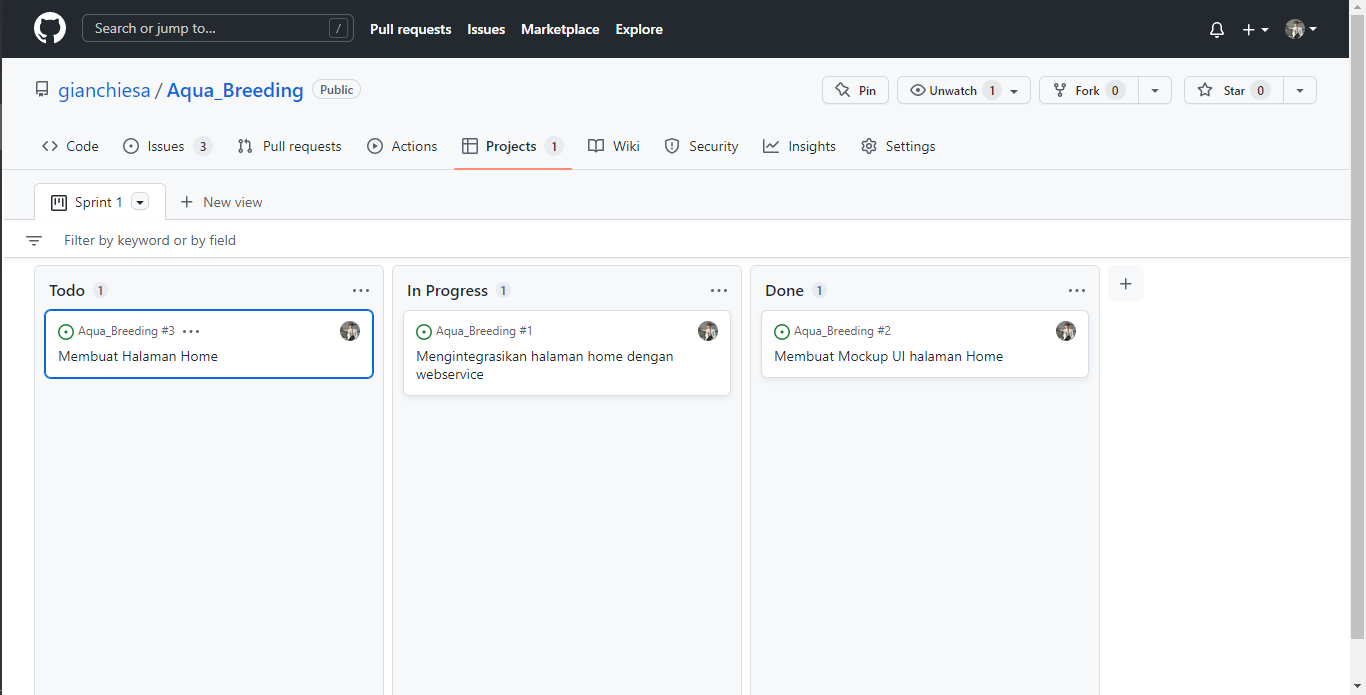
\includegraphics[keepaspectratio, width=14cm]{gambar/githubprojectgian}
	\caption{\textit{Github Projects Sprint-1}}
	\label{gambar:sprint1_projects}
\end{figure}
	
Terdapat 3 kolom pada \textit{project} yang dibuat, yaitu \textit{to do}, \textit{in progress}, dan \textit{completed}. Setiap \textit{task} yang perlu dikerjakan akan ditulis dan dimasukkan ke dalam kolom \textit{to do}, selanjutnya \textit{task} yang sedang dikerjakan akan dipindahkan ke kolom \textit{in progress}, dan jika task sudah selesai akan dipindahkan ke kolom \textit{completed}. Berikut merupakan hasil dari pengerjaan yang dilakukan selama \textit{sprint 1}.

\begin{enumerate}[listparindent=2em]
	
	\item{\textit{Membuat Mock-up UI Halaman Dashboard}}
	
	Pembuatan konten dan fitur yang terdapat pada \textit{mock-up UI} halaman home dilakukan berdasarkan persetujuan product owner dan scrum master pada meeting sebelumnya. Mock-up UI dibuat menggunakan platform figma.
	
	\begin{figure}[H]
	\centering
	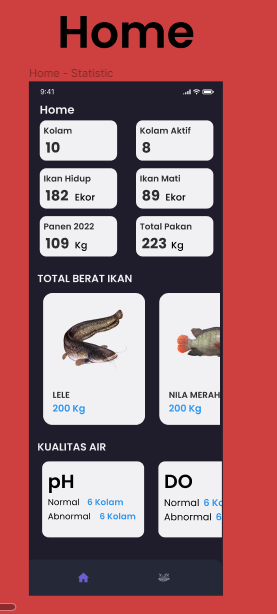
\includegraphics[keepaspectratio, width=4cm]{gambar/mockuphome}
	\caption{\textit{Mock-up UI Halaman Dashboard}}
	\label{gambar:mockuphome}
	\end{figure}

	Lalu selanjutnya dibuat prototype agar product owner dan scrum master dapat lebih mengerti bagaimana konten dan fitur tersebut berjalan saat akan dikembangkan seperti pada gambar \ref{gambar:protohome}.

	\begin{figure}[H]
	\centering
	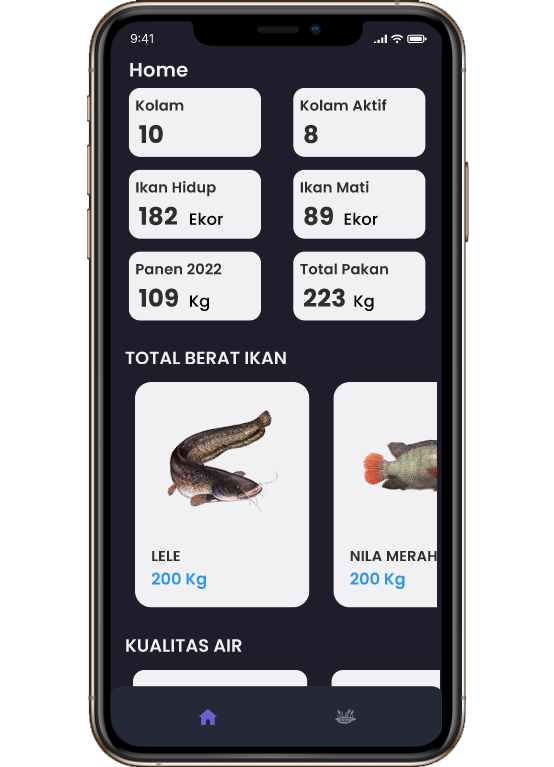
\includegraphics[keepaspectratio, width=5cm]{gambar/protohome}
	\caption{\textit{Prototype Halaman Dashboard}}
	\label{gambar:protohome}
	\end{figure}
	
	\item{\textit{Menetapkan Struktor Direktori}}

	Sebelum menerapkan Mockup-UI kedalam code, penulis membuat atau menetapkan struktur direktori file agar memudahkan penulis untuk melakukan proses pengembangan untuk kedepannya. Terdapat 4 direktori yang penulis buat pada penelitian kal ini, yaitu models, controllers, pages, dan services. Direktori models akan memuat file yang berfungsi sebagai model class, lalu pada direktori contoller berisi file controller-controller yang akan digunakan pada suatu halaman/fitur untuk memanipulasi/mengolah data yang didapat dari services. Direktori services berisi file yang digunakan untuk berinteraksi dengan dunia luar seperti pemanggilan API dan membuat network request, untuk direktori pages memuat file UI halaman.

	\begin{figure}[H]
	\centering
	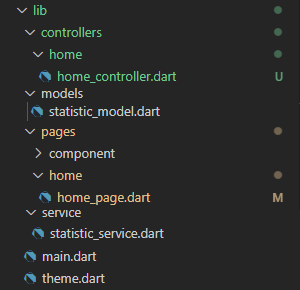
\includegraphics[keepaspectratio, width=7cm]{gambar/homedirektori}
	\caption{\textit{Struktur Direktori}}
	\label{gambar:homedirektori}
	\end{figure}

	\item{\textit{Class Diagram}}
	
	Class Diagram menggambarkan kelas-kelas yang akan dipakai oleh sistem. Umumnya terdapat 3 kelas pada setiap module yaitu class model, controller, dan view. Pada sprint-1 penelitian kali ini penulis membuat 4 class yaitu model, view , controller, dan service.
	 
	\begin{figure}[H]
	\centering
	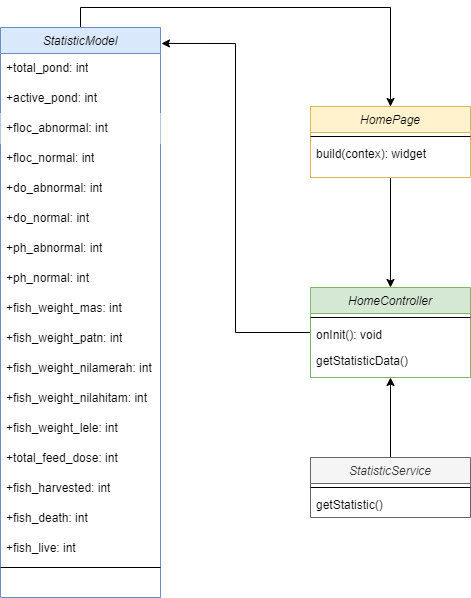
\includegraphics[keepaspectratio, width=6cm]{gambar/CDfishnew}
	\caption{\textit{Class Diagram Sprint-1}}
	\label{gambar:classdiagram}
	\end{figure}

	Pada gambar \ref{gambar:classdiagram} class HomePage sebagai view menginisiasi controller dari interaksi dengan user, lalu controller akan memanggil mengfetch data dari service class dan memasukan data tersebut ke model class, setelah itu model class akan memberi tahu sistem jika data sudah terupdate dan akan mengirimkan data tersebut kembali ke view.

	\item{\textit{Menerapkan Mockup-UI Halaman Dashboard kedalam code flutter}}
	
	Setelah \textit{mock-up UI Halaman Dashboard} hingga prototype dibuat, akan dilakukan pengimplementasian \textit{mock- up UI} ke dalam aplikasi menggukan flutter. Pada lampiran 2 terdapat source code dari implementasi halaman home yang dikelompokan berdasarkan section.

	\item{\textit{Mengitegrasikan Halaman Dashboard dengan webservice}}
	
	Sebelumnya, setiap data pada halaman home masih berupa data dummy sehingga perlu diintegrasikan dengan webservice agar aplikasi dapat berjalan dengan data yang asli. pada lampiran 6 terdapat langkah-langkah untuk mengintegrasikan halaman dashboard dengan webservice.
	

\item{Sprint 1 Review dan Sprint 2 Planning}

Sprint 1 diakhiri dengan melakukan weekly meeting pada hari selasa dengan agenda melakukan review dan testing terkait hasil sprint 1 dan melakukan planning untuk sprint 2 dengan rincian:
\begin{enumerate}
	\item{\textit{Review dan Testing hasil dari sprint 1}}

	Telah dilakukan review dan testing oleh penulis selaku developer dengan Scrum Master. Setelah dilakukan testing, Scrum Master menyimpulkan bahwa fitur pada halaman dashboard telah berjalan dengan baik.

	\begin{longtable}{| p{8cm} | c | c | l |}
		\caption{Unit testing Halaman Dashboard.\label{table:unit_testing_fitur_dashboard}}\\
		\hline
		\multirow{2}{*}{Skenario Pengujian} & \multicolumn{2}{l|}{Kesesuaian} & \multirow{2}{*}{Kesimpulan} \\ 
		\cline{2-3}
		  & \multicolumn{1}{l|}{sesuai} & tidak sesuai & \\ 
		\hline
		\hline
		\endfirsthead
		\hline
		\multirow{2}{*}{Skenario Pengujian} & \multicolumn{2}{l|}{Kesesuaian} & \multirow{2}{*}{Kesimpulan} \\ 
		\cline{2-3}
		  & \multicolumn{1}{l|}{sesuai} & tidak sesuai &  \\ 
		\hline
		\hline
		\endhead
		\hline
		\endfoot
		
		
		\hline\hline
		\endlastfoot
		 Ketika mengisi form login dengan data yang sesuai kemudian menekan submit, maka akan masuk ke halaman dashboard & \Checkmark &  & Diterima \\ 
		\hline
		 Saat tombol kolam ditekan maka akan muncul halaman yang menampilkan list kolam & \Checkmark & & Diterima \\ 
		\hline
		\end{longtable}

	\begin{figure}[H]
	\centering
	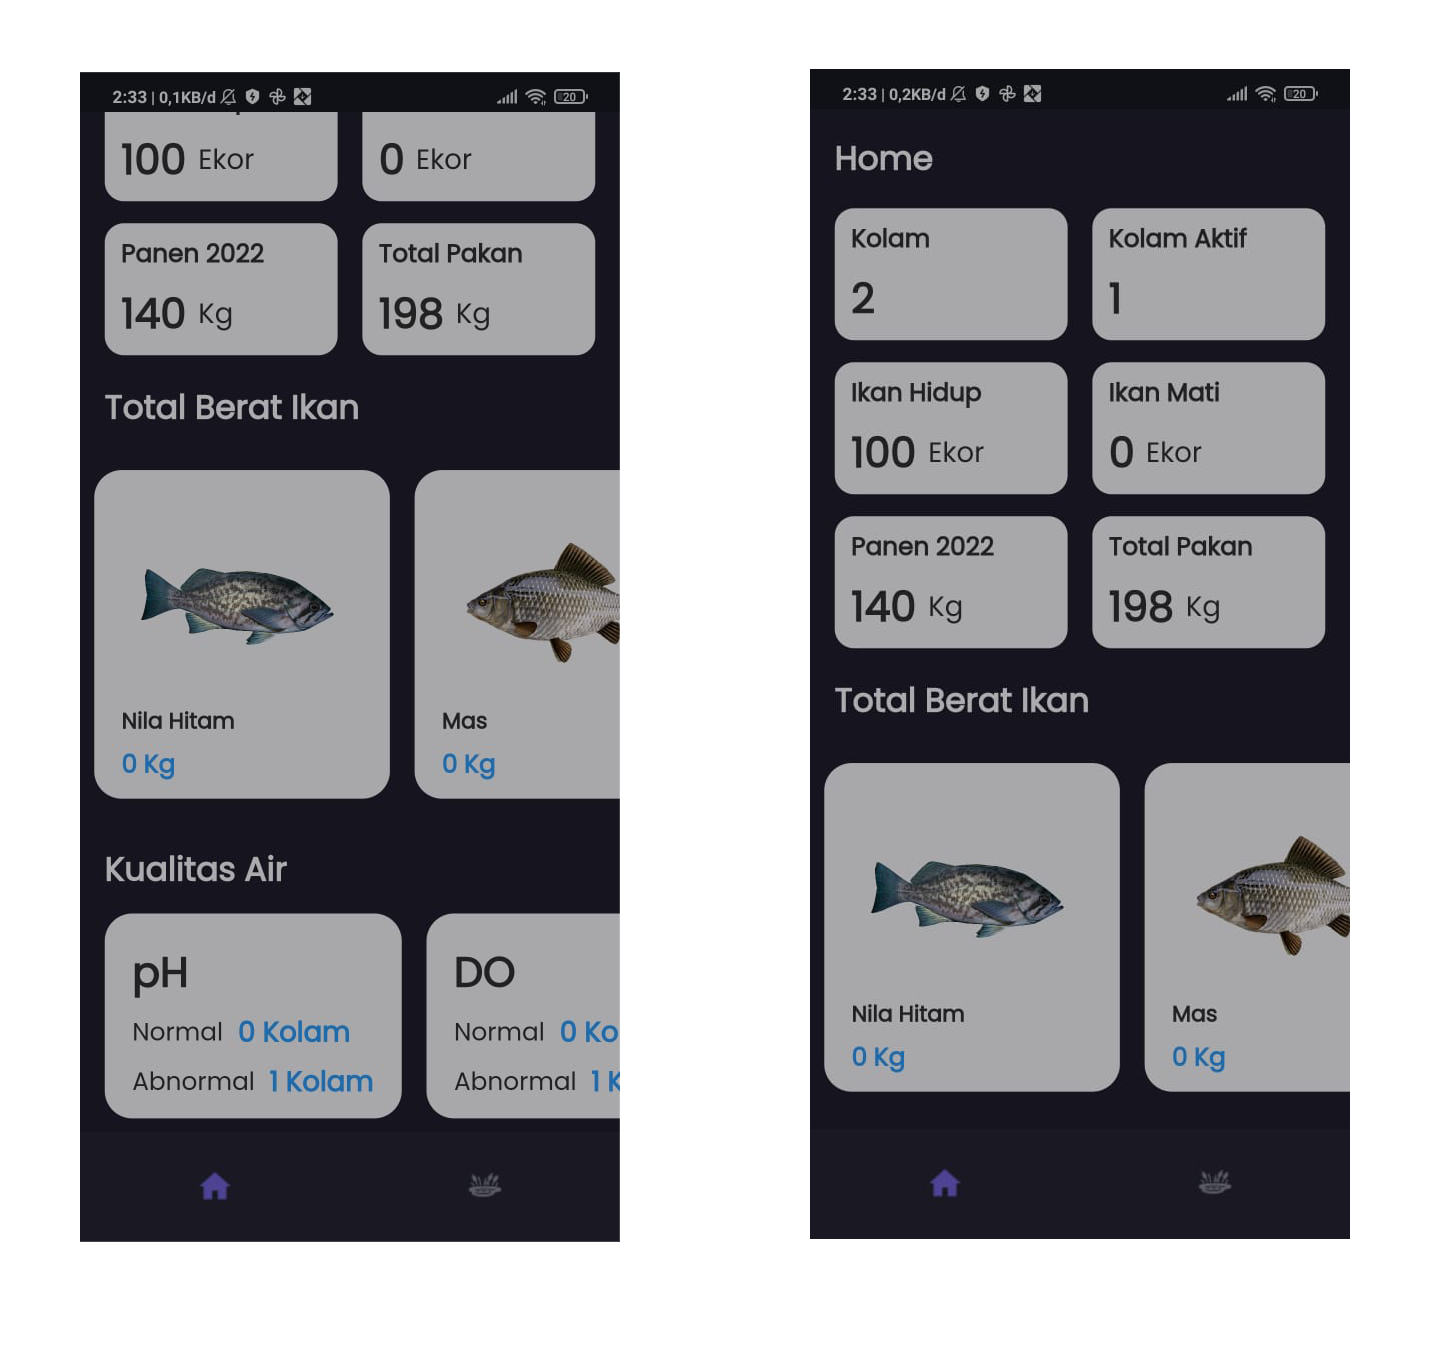
\includegraphics[keepaspectratio, width=7cm]{gambar/ssaqua}
	\caption{\textit{Screenshot dari Halaman Home yang telah selesai}}
	\label{gambar:mockuphome}
	\end{figure}

	\item{\textit{Sprint Planning untuk Sprint 2}}
	
	Planning untuk sprint 2 yakni membuat fitur registrasi kolam dan aktifasi musim budidaya pada aplikasi \textit{Assistive Aquaculture Breeding Management}.
\end{enumerate}
\end{enumerate}
`	
%!TEX root = ./template-skripsi.tex
\subsection{\textit{Sprint 2}}

	\textit{Sprint-2} dilakukan sepekan pada tanggal 30 Agustus 2022 sampai dengan 6 September 2022. \textit{Story} kedua pada \textit{product backlog} yaitu membuat fitur registrasi kolam dan aktivasi musim budidaya dipecah menjadi beberapa \textit{task} sebagai berikut.


 \begin{longtable}[c]{@{} |p{1cm}|p{4cm}|p{5cm}|p{3cm}| @{}}
 \caption{\textit{Sprint 2} \label{sprint2_table}}\\


 \hline
  \multirow{1}{=}{\centering{\textbf{No}}} & \multirow{1}{=}{\centering{\textbf{\textit{Story}}}} & \multirow{1}{=}{\centering{\textbf{\textit{Task}}}} & \multirow{1}{=}{\centering{\textbf{\textit{Status}}}}\\
 \endfirsthead

 \hline
  \multirow{1}{=}{\centering{\textbf{No}}} & \multirow{1}{=}{\centering{\textbf{\textit{Story}}}} & \multirow{1}{=}{\centering{\textbf{\textit{Task}}}} & \multirow{1}{=}{\centering{\textbf{\textit{Status}}}}\\
 \endhead

 \hline
 \endfoot

 \hline
 \endlastfoot

 \hline
 1 & Membuat fitur registrasi kolam dan aktivasi musim budidaya &  Membuat \textit{Mock-up UI} halaman list kolam, registrasi kolam, detail kolam, aktivasi dan deaktivasi kolam &  selesai \\
 \hline
 2 & & Menerapkan struktur direktori dan membuat class diagram & selesai\\
 \hline
 3 & & Menerapkan \textit{Mock-up UI}  halaman list kolam, registrasi kolam, detail kolam, aktivasi dan deaktivasi kolam & selesai\\
 \hline
 4 & & Mengintegrasikan halaman list kolam, registrasi kolam, detail kolam, aktivasi dan deaktivasi kolam ke \textit{webservice} & next sprint\\
 \hline
 \end{longtable}

Pada sprint ini story yang di pilih untuk di uraikan pada sprint kali ini adalah membuat fitur registrasi kolam dan aktivasi musim budidaya . Tujuan dari \textit{sprint-2} ini adalah membuat halaman list kolam, registrasi kolam, detail kolam, aktivasi dan deaktivasi kolam dan mengintegrasikan halaman tersebut dengan webservice. Kendala yang dialami penilis pada sprint kali ini adalah banyaknya fitur yang harus di aplikasikan sehingga ada task yang harus dilanjukan pada sprint berikutnya. Berikut merupakan hasil dari pengerjaan yang dilakukan selama \textit{sprint 2}.

\begin{enumerate}[listparindent=2em]
	
	\item{\textit{Membuat Mock-up UI Halaman List kolam, Registrasi kolam, Detail kolam, Aktivasi dan Deaktivasi kolam}}
	
	Pembuatan konten dan fitur yang terdapat pada \textit{mock-up UI} halaman list kolam, registrasi kolam, detail kolam, aktivasi dan deaktivasi kolam dilakukan berdasarkan persetujuan product owner dan scrum master pada meeting sebelumnya. Mock-up UI dibuat menggunakan platform figma.
	
	\begin{figure}[H]
	\centering
	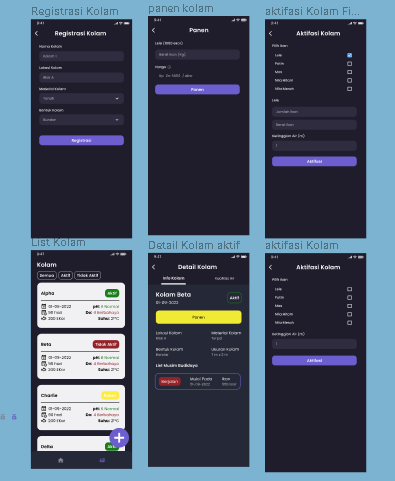
\includegraphics[keepaspectratio, width=4cm]{gambar/mockupsprint2}
	\caption{\textit{Mock-up UI List kolam, Registrasi kolam, Detail kolam, Aktivasi dan Deaktivasi kolam}}
	\label{gambar:mockupsprint2}
	\end{figure}

	\item{\textit{Class Diagram}}
	
	Class Diagram menggambarkan kelas-kelas yang akan dipakai oleh sistem. Umumnya terdapat 3 kelas pada setiap module yaitu class model, controller, dan view. Pada sprint-2 penelitian kali ini penulis membuat 4 class yaitu model yang berwarna biru, view berwarna oranye, controller yang berwarna hijau, dan service yang berwarna kuning.
	 
	 \begin{figure}[H]
	 \centering
	 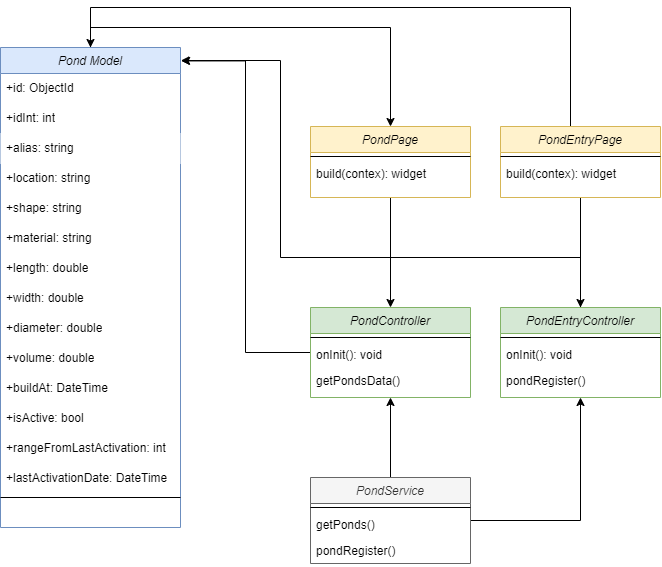
\includegraphics[keepaspectratio, width=6cm]{gambar/pondcd}
	 \caption{\textit{Class Diagram Fitur Koam Sprint-2}}
	 \label{gambar:pondcd}
	 \end{figure}

	 \begin{figure}[H]
	 \centering
	 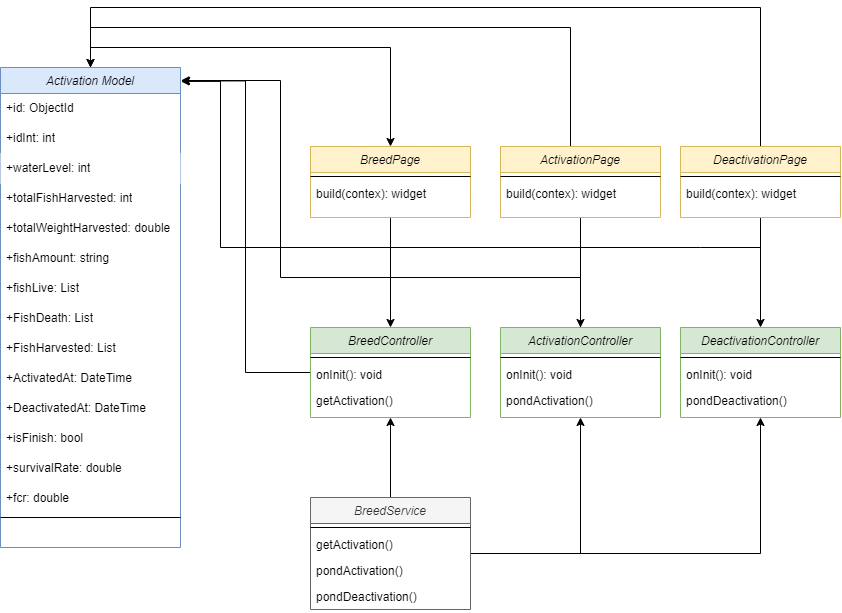
\includegraphics[keepaspectratio, width=6cm]{gambar/activationcd}
	 \caption{\textit{Class Diagram Fitur Aktivasi dan Deaktivasi Sprint-2}}
	 \label{gambar:activationcd}
	 \end{figure}

	\item{\textit{Menerapkan mockup-UI  halaman list kolam, registrasi kolam, detail kolam, aktivasi dan deaktivasi kedalam code flutter}}
	
	Setelah \textit{mock-up UI  halaman list kolam, registrasi kolam, detail kolam, aktivasi dan deaktivasi} dibuat, akan dilakukan pengimplementasian \textit{mock- up UI} ke dalam aplikasi menggukan flutter. Berikut adalah source code dari implementasi halaman list kolam, registrasi kolam, detail kolam, aktivasi dan deaktivasi yang terdapat pada lampiran 3 dan menghasilkan output halaman sebagai berikut

	\begin{figure}[H]
	\centering
	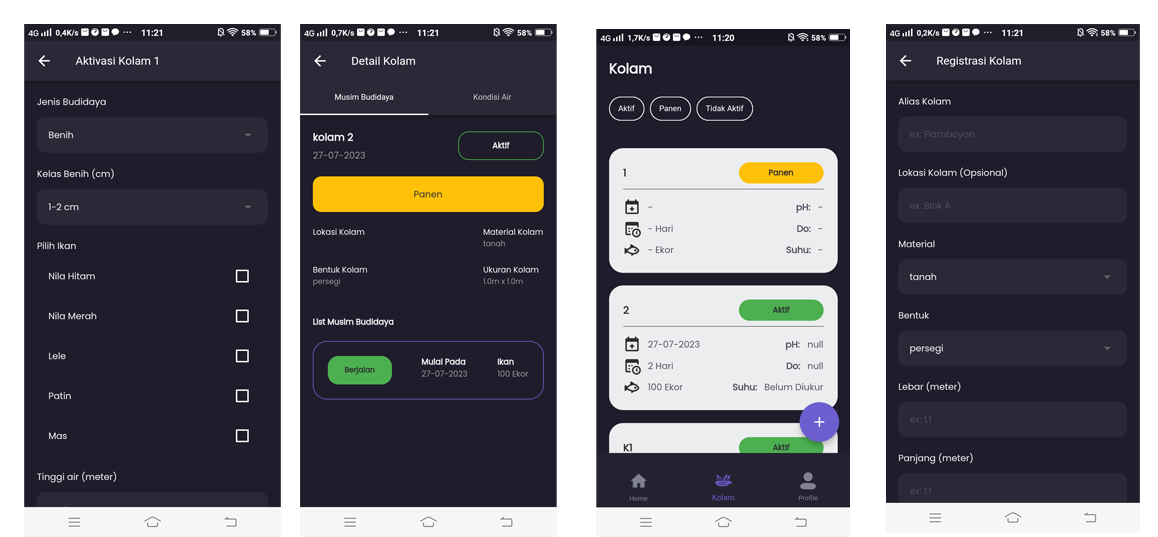
\includegraphics[keepaspectratio, width=8cm]{gambar/sssprint2}
	\caption{\textit{Output dari code pada sprint 2}}
	\label{gambar:sssprint4}
	\end{figure}

\item{Analisis \textit{User Experience}} 
 
pada halaman halaman list kolam terdapat card yang berisi informasi yang berguna bagi para pembudidaya untuk melakukan pemantauan terkait aktivitas yang terdapat pada masing-masing kolam. Sementara pada halaman registrasi kolam, pembudidaya harus memasukan data yang diperlukan untuk menambahkan kolam sesuai dengan kesepakatan saat meeting. Lalu pada halaman detail kolam terdapat data kolam terkait dan list musim budidaya yang telah berjalan di kolam tersebut. Sama halnya dengan aktivasi dan deaktivasi pembudidaya harus memasukan data yang diperlukan sesuai dengan kesepakatan saat meeting.


\item{Sprint 2 Review dan Sprint 3 Planning}

Sprint 2 diakhiri dengan melakukan weekly meeting pada hari selasa dengan agenda melakukan review dan testing terkait hasil sprint 2 dan melakukan planning untuk sprint 3 dengan rincian:
\begin{enumerate}
	\item{\textit{Review dan Testing hasil dari sprint 2}}

	Telah dilakukan review dan testing oleh penulis selaku developer dengan Scrum Master. Setelah dilakukan testing, Scrum Master menyimpulkan bahwa penerapan fitur pada halaman list kolam, detail kolam, aktivasi kolam, deaktivasi kolam telah berjalan dengan baik namun belum di integrasikan dengan data dari API sehingga akan dilanjutkan kedalam sprint berikutnya.

	\item{\textit{Sprint Planning untuk Sprint 3}}
	
	Planning untuk sprint 3 yakni membuat fitur pemberian pakan pada aplikasi \textit{Assistive Aquaculture Breeding Management}.
\end{enumerate}
\end{enumerate}
%!TEX root = ./template-skripsi.tex
\subsection{\textit{Sprint 3}}

	\textit{Sprint-3} dilakukan sepekan pada tanggal 6 September 2022 sampai dengan 13 September 2022. \textit{Story} ketiga  pada \textit{product backlog} yaitu membuat fitur pemberian pakan, ditambah dengan melanjutkan bagian yang belum selesai dari sprint sebelumnya yaitu mengintegrasikan halaman list kolam, registrasi kolam, aktivasi kolam, dan deaktivasi kolam dipecah menjadi beberapa \textit{task} sebagai berikut.


 \begin{longtable}[c]{@{} |p{1cm}|p{4cm}|p{5cm}|p{3cm}| @{}}
 \caption{\textit{Sprint 3} \label{sprint3_table}}\\


 \hline
  \multirow{1}{=}{\centering{\textbf{No}}} & \multirow{1}{=}{\centering{\textbf{\textit{Story}}}} & \multirow{1}{=}{\centering{\textbf{\textit{Task}}}} & \multirow{1}{=}{\centering{\textbf{\textit{Status}}}}\\
 \endfirsthead

 \hline
  \multirow{1}{=}{\centering{\textbf{No}}} & \multirow{1}{=}{\centering{\textbf{\textit{Story}}}} & \multirow{1}{=}{\centering{\textbf{\textit{Task}}}} & \multirow{1}{=}{\centering{\textbf{\textit{Status}}}}\\
 \endhead

 \hline
 \endfoot

 \hline
 \endlastfoot

 \hline
 1 & Melanjutkan bagian yang belum selesai dari sprint sebelumnya &  Mengintegrasikan halaman list kolam, registrasi kolam, aktivasi kolam, dan deaktivasi kolamm &  selesai \\
 \hline
 2 & Membuat fitur pemberian pakan & Membuat mockup-UI untuk fitur pemberian pakan & selesai\\
 \hline
 3 & & Menerapkan \textit{Mock-up UI} halaman pemberian pakan & selesai\\
 \hline
 4 & & Mengintegrasikan halaman pemberian pakan ke \textit{webservice} & selesai\\
 \hline
 \end{longtable}

Pada \textit{sprint-3} ini, story yang dipilih untuk diuraikan adalah membuat fitur pemberian pakan pada kolam budidaya. Tujuan dari \textit{sprint-3} adalah membuat fitur pemberian pakan, serta mengintegrasikan halaman-halaman tersebut dengan webservice. Kendala yang dialami penulis pada \textit{sprint-3} ini adalah banyaknya fitur yang harus diaplikasikan sehingga ada beberapa task yang harus dilanjutkan pada \textit{sprint} berikutnya. Berikut merupakan hasil dari pengerjaan yang dilakukan selama \textit{sprint 3}.

\begin{enumerate}[listparindent=2em]

	\item {\textit{Mengintegrasikan halaman list kolam, registrasi kolam, aktivasi kolam, deaktivasi kolam dengan webservice}}

  sebelumnya data yang terdapat pada halaman list kolam, registrasi kolam, aktivasi kolam, deaktivasi kolam masih berupa data dummy, maka dari itu pada sprint ini penulis perlu mengintegrasikan halaman tersebut dengan web service, code tersebut dapat dilihat pada lampiran 4.


	\item{\textit{Membuat Mock-up UI Halaman Pemberian pakan}}
	
	Pembuatan konten dan fitur yang terdapat pada \textit{mock-up UI} halamanpemberian pakan dilakukan berdasarkan persetujuan product owner dan scrum master pada meeting sebelumnya. Mock-up UI dibuat menggunakan platform figma.
	
	\begin{figure}[H]
	\centering
	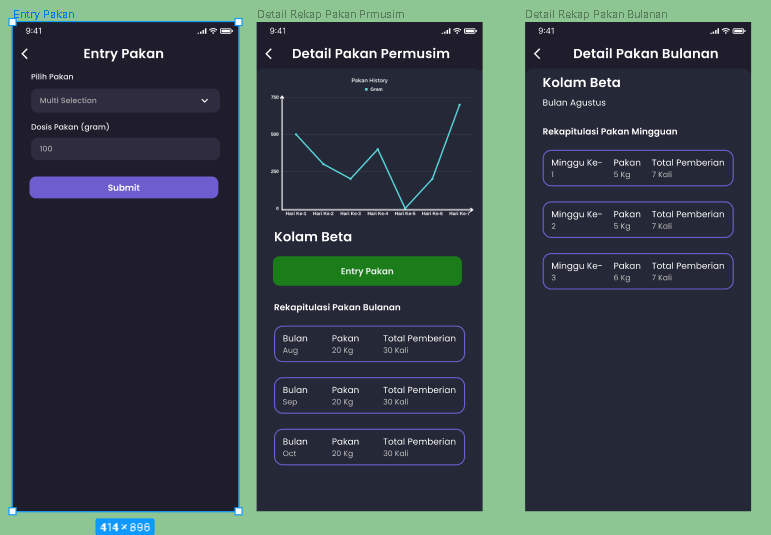
\includegraphics[keepaspectratio, width=4cm]{gambar/ssmockuppakan}
	\caption{\textit{Mock-up UI pemberian pakan}}
	\label{gambar:mockupsprint3}
	\end{figure}

	\item{\textit{Menerapkan mockup-UI  halaman pemberian pakan, rekapitulasi pakan kedalam code flutter}}
	
	Setelah \textit{mock-up UI  pemberian pakan, rekapitulasi pakan} dibuat, akan dilakukan pengimplementasian \textit{mock- up UI} ke dalam aplikasi menggukan flutter. Berikut adalah source code dari implementasi halaman  pemberian pakan, rekapitulasi pakan yang dikelompokan pada lampiran 4 dan menghasilkan output sebagai berikut.

	\begin{figure}[H]
	\centering
	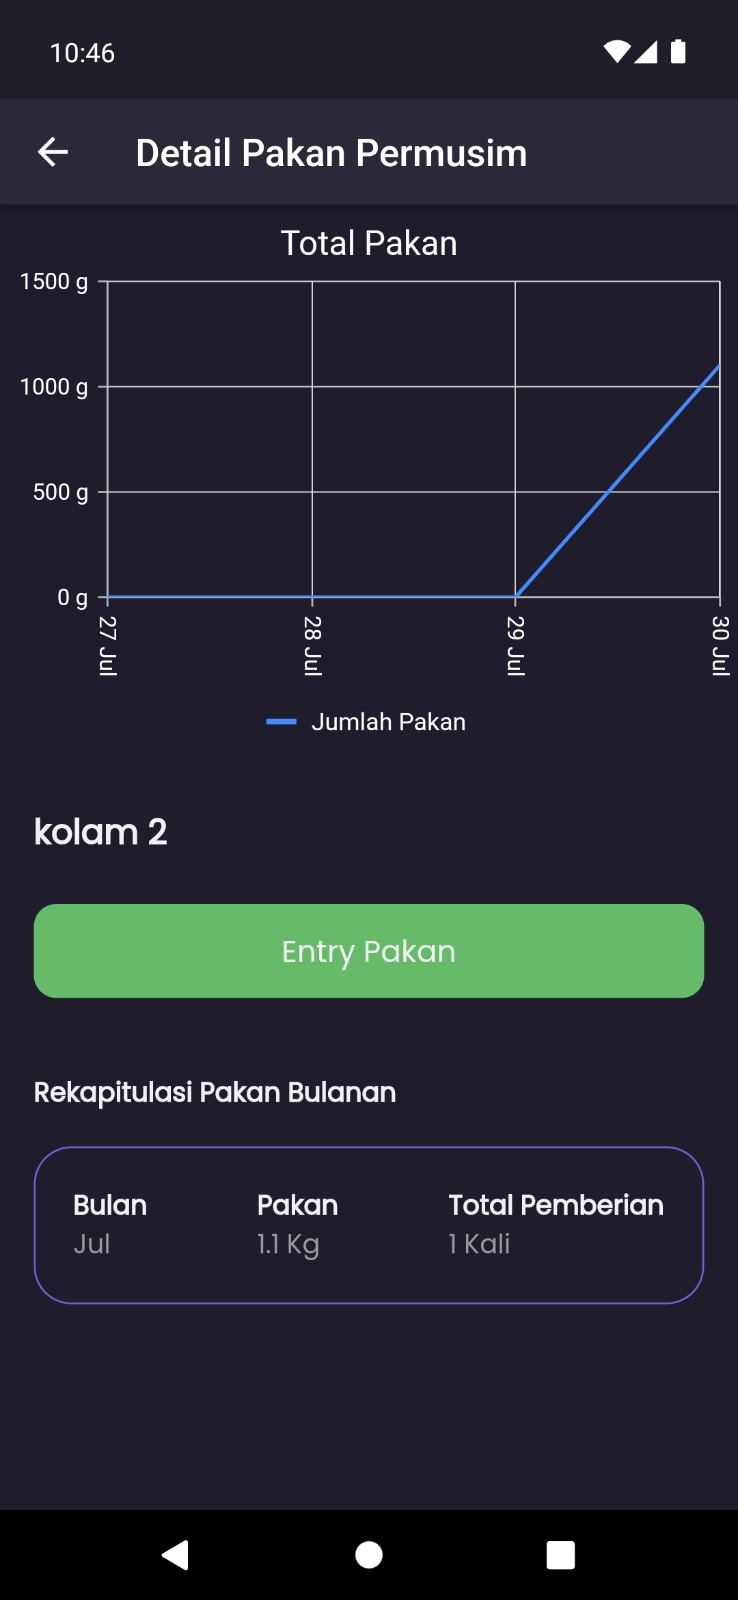
\includegraphics[keepaspectratio, width=3cm]{gambar/ssrekappakan}
	\caption{\textit{Output dari code pada rekapitulasi pakan}}
	\label{gambar:ssrekappakan}
	\end{figure}
	
	\begin{figure}[H]
	\centering
	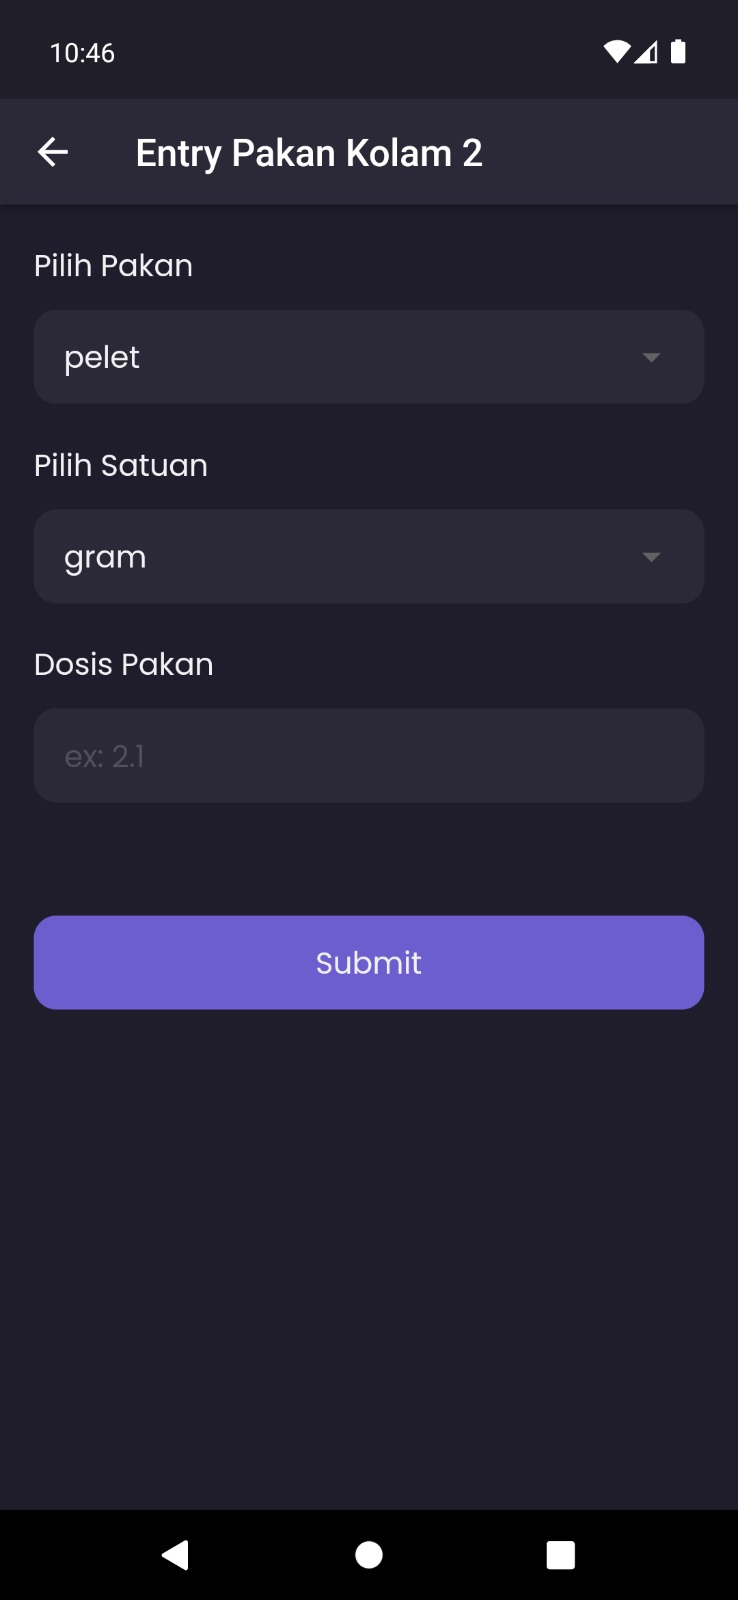
\includegraphics[keepaspectratio, width=4cm]{gambar/ssentrypakan}
	\caption{\textit{Output dari code untuk halaman entry pakan}}
	\label{gambar:ssentrypakan}
	\end{figure}

	\item{\textit{Mengitegrasikan fitur pemberian pakan dengan webservice}}

	Sebelumnya, setiap data pada fitur masih berupa data dummy sehingga perlu diintegrasikan dengan webservice agar aplikasi dapat berjalan dengan data yang asli. Hal yang dilakukan dalam mengintegrasikan fitur pemberian pakan dengan webservice terdapat pada lampiran 4.

  \item{Analisis \textit{User Experience}} 
 
Pada halaman pemberian pakan, pembudidaya harus memasukan dosis pakan dan jenis pakan yang diberikan sehingga data tersbut dapat diolah untuk output FCR nanti saat panen. Di halaman rekapitulasi pakan, terdapat grafik mengenai statistik jumlah pakan yang telah diberikan pada musim budidaya yang berjalan sehingga pembudidaya dapat dengan mudah mengetahui statistik rekap pakan dari setiap musim budidaya yang berjalan, selain itu terdapat juga list mengenai pakan yang telah diberikan yang berisi informasi dosis dan waktu pembudidaya saat memberikan pakan.


\item{Sprint 3 Review dan Sprint 4 Planning}

Sprint 3 diakhiri dengan melakukan weekly meeting pada hari selasa dengan agenda melakukan review dan testing terkait hasil sprint 3 dan melakukan planning untuk sprint 4 dengan rincian:
\begin{enumerate}
	\item{\textit{Review dan Testing hasil dari sprint 3}}

  Telah dilakukan review dan testing oleh penulis selaku developer dengan Scrum Master. Setelah dilakukan testing, Scrum Master menyimpulkan bahwa penerapan fitur pemberian pakan telah berjalan dengan baik.
  
\begin{longtable}{| p{8cm} | c | c | l |}
  \caption{Unit testing Halaman Daftar Kolam.\label{table:unit_testing_fitur_daftar_kolam}}\\
  \hline
  \multirow{2}{*}{Skenario Pengujian} & \multicolumn{2}{l|}{Kesesuaian} & \multirow{2}{*}{Kesimpulan} \\ 
  \cline{2-3}
    & \multicolumn{1}{l|}{sesuai} & tidak sesuai & \\ 
  \hline
  \hline
  \endfirsthead
  \hline
  \multirow{2}{*}{Skenario Pengujian} & \multicolumn{2}{l|}{Kesesuaian} & \multirow{2}{*}{Kesimpulan} \\ 
  \cline{2-3}
    & \multicolumn{1}{l|}{sesuai} & tidak sesuai &  \\ 
  \hline
  \hline
  \endhead
  \hline
  \endfoot
  
  
  \hline\hline
  \endlastfoot
   Saat ikon (+) ditekan maka akan menampilkan halaman registrasi kolam & \Checkmark &  & Diterima \\ 
  \hline
   Saat card kolam ditekan akan menampilkan halaman detail kolam & \Checkmark & & Diterima \\ 
  \hline
  \end{longtable}
  
  \begin{longtable}{| p{8cm} | c | c | l |}
  \caption{Unit testing Halaman Registrasi Kolam.\label{table:unit_testing_fitur_regis_kolam}}\\
  \hline
  \multirow{2}{*}{Skenario Pengujian} & \multicolumn{2}{l|}{Kesesuaian} & \multirow{2}{*}{Kesimpulan} \\ 
  \cline{2-3}
    & \multicolumn{1}{l|}{sesuai} & tidak sesuai & \\ 
  \hline
  \hline
  \endfirsthead
  \hline
  \multirow{2}{*}{Skenario Pengujian} & \multicolumn{2}{l|}{Kesesuaian} & \multirow{2}{*}{Kesimpulan} \\ 
  \cline{2-3}
    & \multicolumn{1}{l|}{sesuai} & tidak sesuai &  \\ 
  \hline
  \hline
  \endhead
  \hline
  \endfoot
  
  
  \hline\hline
  \endlastfoot
   ketika mengisi form registrasi kolam dengan data yang sesuai dan menekan submit, maka kolam baru akan ditambakan & \Checkmark &  & Diterima \\ 
  \hline
  \end{longtable}
  
  \begin{longtable}{| p{8cm} | c | c | l |}
  \caption{Unit testing Halaman Detail Kolam.\label{table:unit_testing_fitur_detail_kolam}}\\
  \hline
  \multirow{2}{*}{Skenario Pengujian} & \multicolumn{2}{l|}{Kesesuaian} & \multirow{2}{*}{Kesimpulan} \\ 
  \cline{2-3}
    & \multicolumn{1}{l|}{sesuai} & tidak sesuai & \\ 
  \hline
  \hline
  \endfirsthead
  \hline
  \multirow{2}{*}{Skenario Pengujian} & \multicolumn{2}{l|}{Kesesuaian} & \multirow{2}{*}{Kesimpulan} \\ 
  \cline{2-3}
    & \multicolumn{1}{l|}{sesuai} & tidak sesuai &  \\ 
  \hline
  \hline
  \endhead
  \hline
  \endfoot
  
  
  \hline\hline
  \endlastfoot
   ketika tombol kualitas air ditekan maka akan menampilkan halaman kualitas air & \Checkmark &  & Diterima \\ 
  \hline
   ketikan menekan salah satu list dari masa budidaya akan menampilkan halaman detail masa budidaya & \Checkmark &  & Diterima \\ 
  \hline
   ketika status kolam tidak aktif atau panen dan menekan tombol start budidaya, maka akan menampilkan halaman aktivasi kolam & \Checkmark &  & Diterima \\ 
  \hline
   ketika status kolam aktif dan menekan tombol aktif, maka akan menampilkan halaman deaktivasi kolam & \Checkmark &  & Diterima \\ 
  \hline
  \end{longtable}
  
  \begin{longtable}{| p{8cm} | c | c | l |}
  \caption{Unit testing Halaman Registrasi Kolam.\label{table:unit_testing_fitur_regis_kolam}}\\
  \hline
  \multirow{2}{*}{Skenario Pengujian} & \multicolumn{2}{l|}{Kesesuaian} & \multirow{2}{*}{Kesimpulan} \\ 
  \cline{2-3}
    & \multicolumn{1}{l|}{sesuai} & tidak sesuai & \\ 
  \hline
  \hline
  \endfirsthead
  \hline
  \multirow{2}{*}{Skenario Pengujian} & \multicolumn{2}{l|}{Kesesuaian} & \multirow{2}{*}{Kesimpulan} \\ 
  \cline{2-3}
    & \multicolumn{1}{l|}{sesuai} & tidak sesuai &  \\ 
  \hline
  \hline
  \endhead
  \hline
  \endfoot
  
  
  \hline\hline
  \endlastfoot
   ketika mengisi form registrasi kolam dengan data yang sesuai dan menekan submit, maka kolam baru akan ditambakan & \Checkmark &  & Diterima \\ 
  \hline
  \end{longtable}
  
  \begin{longtable}{| p{8cm} | c | c | l |}
  \caption{Unit testing Halaman Aktivasi Kolam.\label{table:unit_testing_fitur_aktivasi_kolam}}\\
  \hline
  \multirow{2}{*}{Skenario Pengujian} & \multicolumn{2}{l|}{Kesesuaian} & \multirow{2}{*}{Kesimpulan} \\ 
  \cline{2-3}
    & \multicolumn{1}{l|}{sesuai} & tidak sesuai & \\ 
  \hline
  \hline
  \endfirsthead
  \hline
  \multirow{2}{*}{Skenario Pengujian} & \multicolumn{2}{l|}{Kesesuaian} & \multirow{2}{*}{Kesimpulan} \\ 
  \cline{2-3}
    & \multicolumn{1}{l|}{sesuai} & tidak sesuai &  \\ 
  \hline
  \hline
  \endhead
  \hline
  \endfoot
  
  
  \hline\hline
  \endlastfoot
   ketika mengisi form aktivasi kolam dengan data yang sesuai dan menekan submit, maka musim budidaya baru akan ditambahkan dan status kolam menjadi aktif & \Checkmark &  & Diterima \\ 
  \hline
  \end{longtable}
  
  \begin{longtable}{| p{8cm} | c | c | l |}
  \caption{Unit testing Halaman Deaktivasi Kolam.\label{table:unit_testing_fitur_deaktivasi_kolam}}\\
  \hline
  \multirow{2}{*}{Skenario Pengujian} & \multicolumn{2}{l|}{Kesesuaian} & \multirow{2}{*}{Kesimpulan} \\ 
  \cline{2-3}
    & \multicolumn{1}{l|}{sesuai} & tidak sesuai & \\ 
  \hline
  \hline
  \endfirsthead
  \hline
  \multirow{2}{*}{Skenario Pengujian} & \multicolumn{2}{l|}{Kesesuaian} & \multirow{2}{*}{Kesimpulan} \\ 
  \cline{2-3}
    & \multicolumn{1}{l|}{sesuai} & tidak sesuai &  \\ 
  \hline
  \hline
  \endhead
  \hline
  \endfoot
  
  
  \hline\hline
  \endlastfoot
   ketika mengisi form deaktivasi kolam dengan data yang sesuai dan menekan submit, maka musim budidaya yang barjalan akan berhenti status kolam menjadi tidak aktif & \Checkmark &  & Diterima \\ 
  \hline
  \end{longtable}
  

  \begin{longtable}{| p{8cm} | c | c | l |}
    \caption{Unit testing Halaman Detail Masa Budidaya.\label{table:unit_testing_detail_budidaya}}\\
    \hline
    \multirow{2}{*}{Skenario Pengujian} & \multicolumn{2}{l|}{Kesesuaian} & \multirow{2}{*}{Kesimpulan} \\ 
    \cline{2-3}
      & \multicolumn{1}{l|}{sesuai} & tidak sesuai & \\ 
    \hline
    \hline
    \endfirsthead
    \hline
    \multirow{2}{*}{Skenario Pengujian} & \multicolumn{2}{l|}{Kesesuaian} & \multirow{2}{*}{Kesimpulan} \\ 
    \cline{2-3}
      & \multicolumn{1}{l|}{sesuai} & tidak sesuai &  \\ 
    \hline
    \hline
    \endhead
    \hline
    \endfoot
    
    
    \hline\hline
    \endlastfoot
    Ketika tombol rekapitulasi pakan ditekan, maka akan ditampilkan halaman rekapitulasi pakan & \Checkmark &  & Diterima \\ 
    \hline
    Ketika tombol rekapitulasi kematian ikan ditekan, maka akan ditampilkan halaman rekapitulasi kematian ikan & \Checkmark &  & Diterima \\ 
    \hline
    Ketika tombol rekapitulasi grading ikan ditekan, maka akan ditampilkan halaman rekapitulasi grading ikan & \Checkmark &  & Diterima \\ 
    \hline
    Ketika tombol treatment ditekan, maka akan ditampilkan halaman treatment kolam & \Checkmark &  & Diterima \\ 
    \hline
     Ketika tombol sortir ditekan, maka akan ditampilkan halaman sortir kolam & \Checkmark &  & Diterima \\ 
    \hline
    \end{longtable}
    
    
    \begin{longtable}{| p{8cm} | c | c | l |}
    \caption{Unit testing Halaman Rekapitulasi Pakan.\label{table:unit_testing_rekapitulasi_pakan}}\\
    \hline
    \multirow{2}{*}{Skenario Pengujian} & \multicolumn{2}{l|}{Kesesuaian} & \multirow{2}{*}{Kesimpulan} \\ 
    \cline{2-3}
      & \multicolumn{1}{l|}{sesuai} & tidak sesuai & \\ 
    \hline
    \hline
    \endfirsthead
    \hline
    \multirow{2}{*}{Skenario Pengujian} & \multicolumn{2}{l|}{Kesesuaian} & \multirow{2}{*}{Kesimpulan} \\ 
    \cline{2-3}
      & \multicolumn{1}{l|}{sesuai} & tidak sesuai &  \\ 
    \hline
    \hline
    \endhead
    \hline
    \endfoot
    
    
    \hline\hline
    \endlastfoot
    Ketika menekan list data rekapitulasi pakan, maka akan ditamplikan detail rekapitulasi pakan & \Checkmark &  & Diterima \\ 
    \hline
    Ketika menekan list data rekapitulasi pakan, maka akan ditamplikan detail rekapitulasi pakan & \Checkmark &  & Diterima \\ 
    \hline
    Saat tombol entry pakan ditekan maka akan menampilkan halaman entry pakan & \Checkmark &  & Diterima \\ 
    \hline
     ketika mengisi form rekapitulasi pakan dengan data yang sesuai dan menekan submit, data rekapitulasi pakan akan ditambahkan & \Checkmark &  & Diterima \\ 
    \hline
    \end{longtable}

	\item{\textit{Sprint Planning untuk Sprint 4}}
	
	Planning untuk sprint 4 yakni membuat fitur grading ikan pada aplikasi \textit{Assistive Aquaculture Breeding Management}.
\end{enumerate}
\end{enumerate}
%!TEX root = ./template-skripsi.tex

\subsection{\textit{Sprint 4}}

	\textit{Sprint-4} dilakukan sepekan pada tanggal 13 September 2022 sampai dengan 20 september 2022. \textit{Story} keempat pada \textit{product backlog} yaitu membuat grading berat dipecah menjadi beberapa \textit{task} sebagai berikut.


 \begin{longtable}[c]{@{} |p{1cm}|p{4cm}|p{5cm}|p{3cm}| @{}}
 \caption{\textit{Sprint 4} \label{sprint4_table}}\\


 \hline
  \multirow{1}{=}{\centering{\textbf{No}}} & \multirow{1}{=}{\centering{\textbf{\textit{Story}}}} & \multirow{1}{=}{\centering{\textbf{\textit{Task}}}} & \multirow{1}{=}{\centering{\textbf{\textit{Status}}}}\\
 \endfirsthead

 \hline
  \multirow{1}{=}{\centering{\textbf{No}}} & \multirow{1}{=}{\centering{\textbf{\textit{Story}}}} & \multirow{1}{=}{\centering{\textbf{\textit{Task}}}} & \multirow{1}{=}{\centering{\textbf{\textit{Status}}}}\\
 \endhead

 \hline
 \endfoot

 \hline
 \endlastfoot

 \hline
 1 & Membuat fitur grading berat ikan &  Membuat \textit{Mock-up UI} halaman rekapitulasi grading, detail grading, entry grading  &  selesai \\
 \hline
 2 & & Menerapkan \textit{Mock-up UI} halaman rekapitulasi grading, detail grading, entry grading ke Flutter & selesai\\
 \hline
 3 & & Mengintegrasikan halaman rekapitulasi grading, detail grading, entry grading ke \textit{webservice} & selesai\\
 \hline
 \end{longtable}

Pada sprint keempat ini story yang di pilih untuk di uraikan pada sprint kali ini adalah membuat halaman rekapitulasi grading, detail grading, entry grading. Tujuan dari \textit{sprint-4} ini adalah membuat fitur grading berat ikan dan mengintegrasikan halaman tersebut dengan webservice yang sudah dibuat oleh penelitian Andri Rahmanto.

\begin{enumerate}[listparindent=2em]
	
	\item{\textit{Membuat Mock-up UI Fitur Grading}}
	
	Pembuatan konten dan fitur yang terdapat pada \textit{mock-up UI} fitur grading dilakukan berdasarkan persetujuan product owner dan scrum master pada meeting sebelumnya. Mock-up UI dibuat menggunakan platform figma.
	
	\begin{figure}[H]
	\centering
	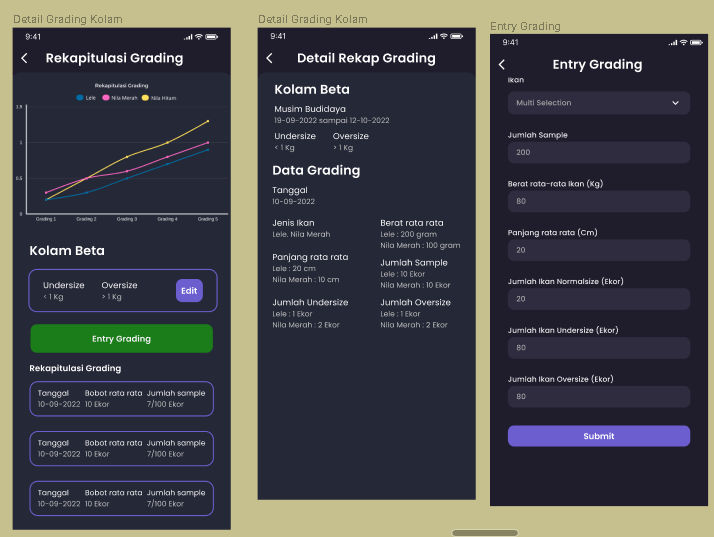
\includegraphics[keepaspectratio, width=6cm]{gambar/mockupgrading}
	\caption{\textit{Mock-up UI Fitur Grading}}
	\label{gambar:mockupgrading}
	\end{figure}

	\item{\textit{Class Diagram}}
	
	Class Diagram menggambarkan kelas-kelas yang akan dipakai oleh sistem. Umumnya terdapat 3 kelas pada setiap module yaitu class model, controller, dan view. Pada sprint-4 penelitian kali ini penulis membuat 4 class yaitu model yang berwarna biru, view berwarna oranye, controller yang berwarna hijau, dan service yang berwarna kuning.
	 
	 \begin{figure}[H]
	 \centering
	 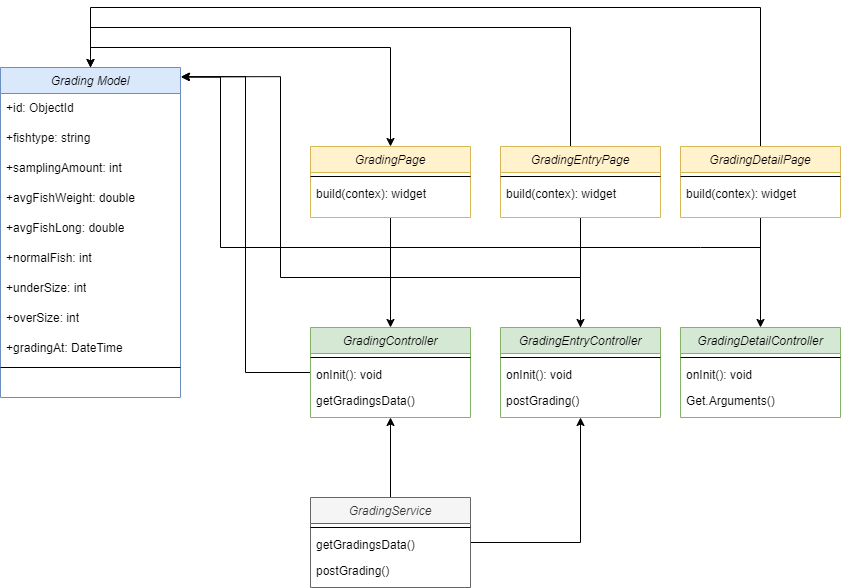
\includegraphics[keepaspectratio, width=6cm]{gambar/gradingcd}
	 \caption{\textit{Class Diagram Fitur Sprint-4}}
	 \label{gambar:gradingcd}
	 \end{figure}


	\item{\textit{Menerapkan Mockup-UI Fitur Grading kedalam code flutter}}
	
	Setelah \textit{mock-up UI fitur grading} hingga prototype dibuat, akan dilakukan pengimplementasian \textit{mock-up UI} ke dalam aplikasi menggukan flutter. Source code dari implementasi fitur grading terdapat pada lampiran 5 yang menghasilkan output halaman sebagai berikut
	
	\begin{figure}[H]
		\centering
		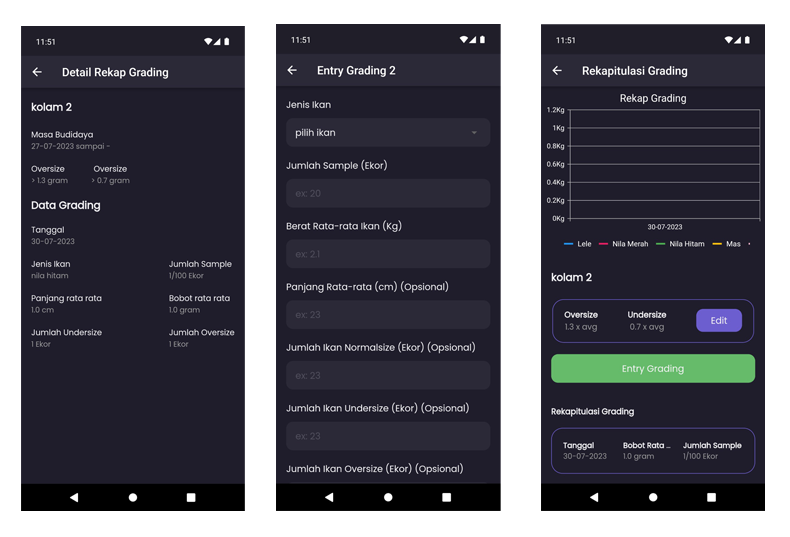
\includegraphics[keepaspectratio, width=8cm]{gambar/sssprint4}
		\caption{\textit{Output dari code pada sprint 4}}
		\label{gambar:sssprint4}
		\end{figure}

	\item{\textit{Mengitegrasikan fitur grading dengan webservice}}

	Sebelumnya, setiap data pada fitur masih berupa data dummy sehingga perlu diintegrasikan dengan webservice agar aplikasi dapat berjalan dengan data yang asli. Hal yang dilakukan dalam mengintegrasikan fitur grading dengan webservice terdapat pada lampiran 5.
	
  \item{Analisis \textit{User Experience}} 
 
  Pada halaman grading, pembudidaya harus jenis ikan dan data klasifikasi ukuran ikan. Di halaman rekapitulasi grading, terdapat grafik mengenai statistik pertumbuhan ikan  pada musim budidaya yang berjalan sehingga pembudidaya dapat dengan mudah mengetahui perkembangan ukuran ikan dari waktu ke waktu, selain itu terdapat juga list mengenai grading yang telah dilakukan yang berisi informasi yang berhubungan dengan ukuran ikan saat dilakukan grading.

\item{Sprint 4 Review dan Sprint 5 Planning}

Sprint 4 diakhiri dengan melakukan weekly meeting pada hari selasa dengan agenda melakukan review dan testing terkait hasil sprint 4 dan melakukan planning untuk sprint 5 dengan rincian:
\begin{enumerate}
	\item{\textit{Review dan Testing hasil dari sprint 4}}

	Telah dilakukan review dan testing oleh penulis selaku developer dengan Scrum Master. Setelah dilakukan testing, Scrum Master menyimpulkan bahwa fitur grading berat ikan telah berjalan dengan baik.
\begin{longtable}{| p{8cm} | c | c | l |}
  \caption{Unit testing Halaman Rekapitulasi Grading.\label{table:unit_testing_rekapitulasi_grading}}\\
  \hline
  \multirow{2}{*}{Skenario Pengujian} & \multicolumn{2}{l|}{Kesesuaian} & \multirow{2}{*}{Kesimpulan} \\ 
  \cline{2-3}
    & \multicolumn{1}{l|}{sesuai} & tidak sesuai & \\ 
  \hline
  \hline
  \endfirsthead
  \hline
  \multirow{2}{*}{Skenario Pengujian} & \multicolumn{2}{l|}{Kesesuaian} & \multirow{2}{*}{Kesimpulan} \\ 
  \cline{2-3}
    & \multicolumn{1}{l|}{sesuai} & tidak sesuai &  \\ 
  \hline
  \hline
  \endhead
  \hline
  \endfoot
  
  
  \hline\hline
  \endlastfoot
  Ketika menekan list data rekapitulasi grading, maka akan ditamplikan detail rekapitulasi grading & \Checkmark &  & Diterima \\ 
  \hline
  Ketika menekan list data rekapitulasi grading, maka akan ditamplikan detail rekapitulasi grading & \Checkmark &  & Diterima \\ 
  \hline
  Saat tombol entry grading ditekan maka akan menampilkan halaman entry grading & \Checkmark &  & Diterima \\ 
  \hline
  ketika mengisi form rekapitulasi grading dengan data yang sesuai dan menekan submit, data rekapitulasi grading akan ditambahkan & \Checkmark &  & Diterima \\ 
  \hline
  \end{longtable}

	\item{\textit{Sprint Planning untuk Sprint 5}}
	
	Planning untuk sprint 5 yakni membuat fitur rekapitulasi kematian ikan pada aplikasi \textit{Assistive Aquaculture Breeding Management}.
\end{enumerate}
\end{enumerate}	
%!TEX root = ./template-skripsi.tex

\subsection{\textit{Sprint 5}}

	\textit{Sprint-5} dilakukan sepekan pada tanggal 20 September 2022 sampai dengan 27 september 2022. \textit{Story} kelimat pada \textit{product backlog} yaitu membuat fitur rekapitulasi kematian ikan dipecah menjadi beberapa \textit{task} sebagai berikut.


 \begin{longtable}[c]{@{} |p{1cm}|p{4cm}|p{5cm}|p{3cm}| @{}}
 \caption{\textit{Sprint 5} \label{sprint5_table}}\\


 \hline
  \multirow{1}{=}{\centering{\textbf{No}}} & \multirow{1}{=}{\centering{\textbf{\textit{Story}}}} & \multirow{1}{=}{\centering{\textbf{\textit{Task}}}} & \multirow{1}{=}{\centering{\textbf{\textit{Status}}}}\\
 \endfirsthead

 \hline
  \multirow{1}{=}{\centering{\textbf{No}}} & \multirow{1}{=}{\centering{\textbf{\textit{Story}}}} & \multirow{1}{=}{\centering{\textbf{\textit{Task}}}} & \multirow{1}{=}{\centering{\textbf{\textit{Status}}}}\\
 \endhead

 \hline
 \endfoot

 \hline
 \endlastfoot

 \hline
 1 & Membuat fitur rekapitulasi kematian ikan &  Membuat \textit{Mock-up UI} halaman rekapitulasi kematian ikan, entry kematian ikan  &  selesai \\
 \hline
 2 & & Menerapkan \textit{Mock-up UI} halaman rekapitulasi kematian ikan, entry kematian ikan ke Flutter & selesai\\
 \hline
 3 & & Mengintegrasikan halaman rekapitulasi kematian ikan, entry kematian ikan ke \textit{webservice} & selesai\\
 \hline
 \end{longtable}

Pada sprint kelima ini story yang di pilih untuk di uraikan pada sprint kali ini adalah membuat halaman rekapitulasi kematian ikan, entry kematian ikan. Tujuan dari \textit{sprint-5} ini adalah membuat fitur rekapitulasi kematian ikan dan mengintegrasikan halaman tersebut dengan webservice yang sudah dibuat oleh penelitian Andri Rahmanto.

\begin{enumerate}[listparindent=2em]
	
	\item{\textit{Membuat Mock-up UI Fitur Rekapitulasi Kematian Ikan}}
	
	Pembuatan konten dan fitur yang terdapat pada \textit{mock-up UI} fitur rekapitulasi kematian ikan dilakukan berdasarkan persetujuan product owner dan scrum master pada meeting sebelumnya. Mock-up UI dibuat menggunakan platform figma.
	
	\begin{figure}[H]
	\centering
	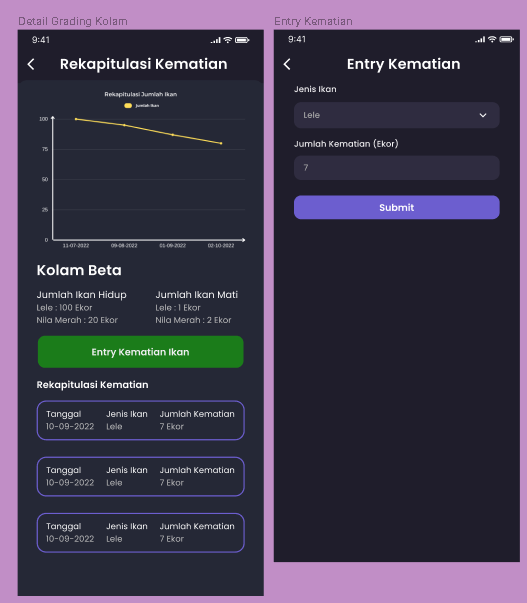
\includegraphics[keepaspectratio, width=6cm]{gambar/mockupkematian}
	\caption{\textit{Mock-up UI Fitur Rekapitulasi Kematian Ikan}}
	\label{gambar:mockupkematian}
	\end{figure}

	\item{\textit{Class Diagram}}
	
	Class Diagram menggambarkan kelas-kelas yang akan dipakai oleh sistem. Umumnya terdapat 3 kelas pada setiap module yaitu class model, controller, dan view. Pada sprint-5 penelitian kali ini penulis membuat 4 class yaitu model yang berwarna biru, view berwarna oranye, controller yang berwarna hijau, dan service yang berwarna kuning.
	 
	 \begin{figure}[H]
	 \centering
	 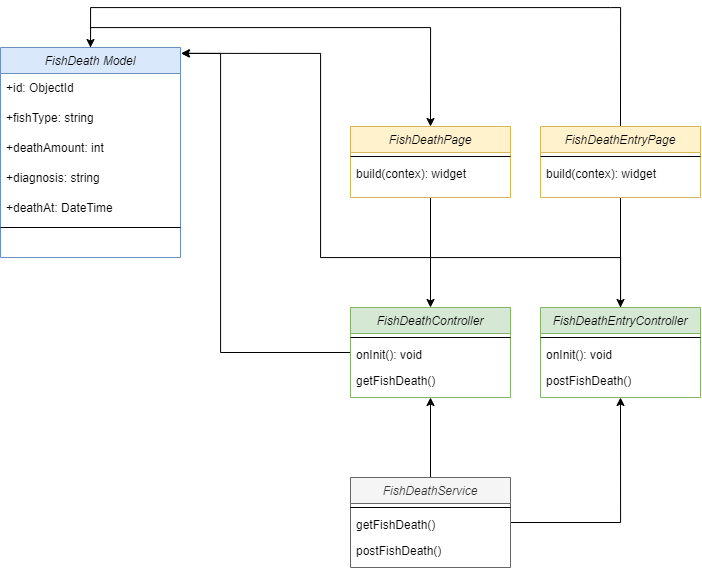
\includegraphics[keepaspectratio, width=6cm]{gambar/deathcd}
	 \caption{\textit{Class Diagram Fitur Sprint-5}}
	 \label{gambar:deathcd}
	 \end{figure}

	\item{\textit{Menerapkan Mockup-UI fitur rekapitulasi kematian ikan kedalam code flutter}}
	
	Setelah itu, akan dilakukan pengimplementasian \textit{mock-up UI} ke dalam aplikasi menggukan flutter. Pada lampiran 6 source code dari implementasi fitur grading yang dikelompokan berdasarkan halaman yang menghasilkan output halaman seperti dibawah ini.

	\begin{figure}[H]
		\centering
		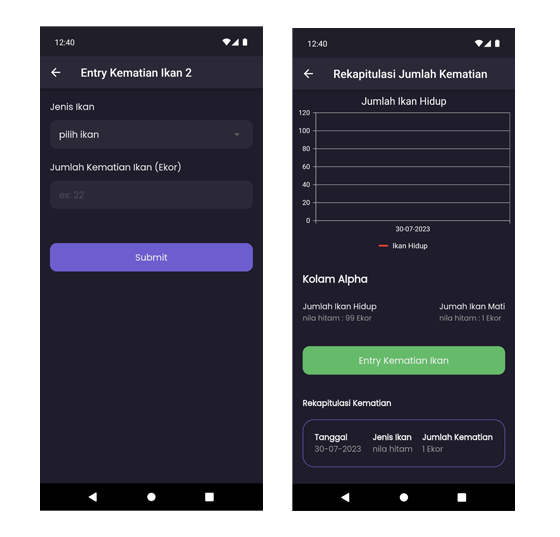
\includegraphics[keepaspectratio, width=8cm]{gambar/sssprint5}
		\caption{\textit{Output dari code pada sprint 5}}
		\label{gambar:sssprint5}
		\end{figure}

	\item{\textit{Mengitegrasikan fitur rekapitulasi kematian dengan webservice}}

	Sebelumnya, setiap data pada fitur masih berupa data dummy sehingga perlu diintegrasikan dengan webservice agar aplikasi dapat berjalan dengan data yang asli. Hal yang dilakukan dalam mengintegrasikan fitur rekapitulasi kematian ikan dengan webservice terdapat pada lampiran 6.

  \item{Analisis \textit{User Experience}} 
 
  Pada halaman entry rekapitulasi kematian, pembudidaya harus jenis ikan dan data jumlah kematian. Di halaman rekapitulasi kematian, terdapat grafik mengenai statistik jumlah ikan  pada musim budidaya yang berjalan sehingga pembudidaya dapat dengan mudah mengetahui penurunan jumlah ikan akibat kematian. Selain itu terdapat juga list mengenai data kematian yang telah dimasukan yang berisi informasi yang berhubungan dengan kematian ikan.

\item{Sprint 5 Review dan Sprint 6 Planning}

Sprint 5 diakhiri dengan melakukan weekly meeting pada hari selasa dengan agenda melakukan review dan testing terkait hasil sprint 5 dan melakukan planning untuk sprint 6 dengan rincian:
\begin{enumerate}
	\item{\textit{Review dan Testing hasil dari sprint 5}}

	Telah dilakukan review dan testing oleh penulis selaku developer dengan Scrum Master. Setelah dilakukan testing, Scrum Master menyimpulkan bahwa fitur rekapitulasi kematian ikan telah berjalan dengan baik.
	
  \begin{longtable}{| p{8cm} | c | c | l |}
    \caption{Unit testing Halaman Rekapitulasi Kematian.\label{table:unit_testing_rekapitulasi_kematian}}\\
    \hline
    \multirow{2}{*}{Skenario Pengujian} & \multicolumn{2}{l|}{Kesesuaian} & \multirow{2}{*}{Kesimpulan} \\ 
    \cline{2-3}
      & \multicolumn{1}{l|}{sesuai} & tidak sesuai & \\ 
    \hline
    \hline
    \endfirsthead
    \hline
    \multirow{2}{*}{Skenario Pengujian} & \multicolumn{2}{l|}{Kesesuaian} & \multirow{2}{*}{Kesimpulan} \\ 
    \cline{2-3}
      & \multicolumn{1}{l|}{sesuai} & tidak sesuai &  \\ 
    \hline
    \hline
    \endhead
    \hline
    \endfoot
    
    
    \hline\hline
    \endlastfoot
    Ketika menekan list data rekapitulasi pakan, maka akan ditamplikan detail rekapitulasi pakan & \Checkmark &  & Diterima \\ 
    \hline
    Saat tombol entry kematian ditekan maka akan menampilkan halaman entry kematian & \Checkmark &  & Diterima \\ 
    \hline
    ketika mengisi form rekapitulasi kematian dengan data yang sesuai dan menekan submit, data rekapitulasi kematian akan ditambahkan & \Checkmark &  & Diterima \\ 
    \hline
    \end{longtable}

	\item{\textit{Sprint Planning untuk Sprint 6}}
	
	Planning untuk sprint 6 yakni membuat fitur treatment kolam pada aplikasi \textit{Assistive Aquaculture Breeding Management}.
\end{enumerate}
\end{enumerate}
%!TEX root = ./template-skripsi.tex

\subsection{\textit{Sprint 6}}

	\textit{Sprint-6} dilakukan sepekan pada tanggal 27 September 2022 sampai dengan 4 oktober 2022. \textit{Story} keenam pada \textit{product backlog} yaitu membuat fitur treatment kolam dipecah menjadi beberapa \textit{task} sebagai berikut.


 \begin{longtable}[c]{@{} |p{1cm}|p{4cm}|p{5cm}|p{3cm}| @{}}
 \caption{\textit{Sprint 6} \label{sprint6_table}}\\


 \hline
  \multirow{1}{=}{\centering{\textbf{No}}} & \multirow{1}{=}{\centering{\textbf{\textit{Story}}}} & \multirow{1}{=}{\centering{\textbf{\textit{Task}}}} & \multirow{1}{=}{\centering{\textbf{\textit{Status}}}}\\
 \endfirsthead

 \hline
  \multirow{1}{=}{\centering{\textbf{No}}} & \multirow{1}{=}{\centering{\textbf{\textit{Story}}}} & \multirow{1}{=}{\centering{\textbf{\textit{Task}}}} & \multirow{1}{=}{\centering{\textbf{\textit{Status}}}}\\
 \endhead

 \hline
 \endfoot

 \hline
 \endlastfoot

 \hline
 1 & Membuat fitur treatment kolam &  Membuat \textit{Mock-up UI} halaman list treatment, detail treatment, entry treatment &  selesai \\
 \hline
 2 & & Menerapkan \textit{Mock-up UI} halaman list treatment, detail treatment, entry treatment  ke Flutter & selesai\\
 \hline
 \end{longtable}

Pada sprint keenam ini story yang di pilih untuk di uraikan pada sprint kali ini adalah membuat halaman rekapitulasi treatment, detail treatment, entry treatment. Tujuan dari \textit{sprint-6} ini adalah membuat fitur treatment berat ikan dan mengintegrasikan halaman tersebut dengan webservice yang sudah dibuat oleh penelitian Andri Rahmanto.
	


\begin{enumerate}[listparindent=2em]
	
	\item{\textit{Membuat Mock-up UI Fitur Treatment Kolam}}
	
	Pembuatan konten dan fitur yang terdapat pada \textit{mock-up UI} fitur treatment kolam dilakukan berdasarkan persetujuan product owner dan scrum master pada meeting sebelumnya. Mock-up UI dibuat menggunakan platform figma.
	
	\begin{figure}[H]
	\centering
	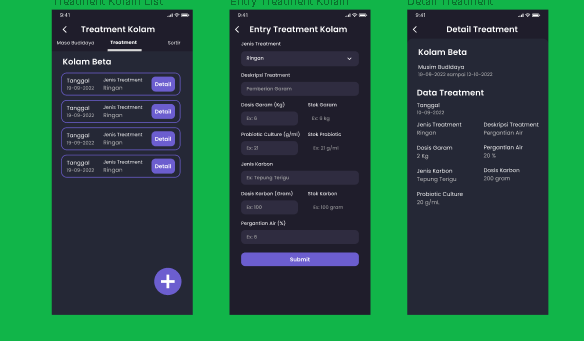
\includegraphics[keepaspectratio, width=6cm]{gambar/mockuptreatment}
	\caption{\textit{Mock-up UI Fitur treatment}}
	\label{gambar:mockuptreatment}
	\end{figure}

	\item{\textit{Class Diagram}}
	
	Class Diagram menggambarkan kelas-kelas yang akan dipakai oleh sistem. Umumnya terdapat 3 kelas pada setiap module yaitu class model, controller, dan view. Pada sprint-6 penelitian kali ini penulis membuat 4 class yaitu model yang berwarna biru, view berwarna oranye, controller yang berwarna hijau, dan service yang berwarna kuning.
	 
	 \begin{figure}[H]
	 \centering
	 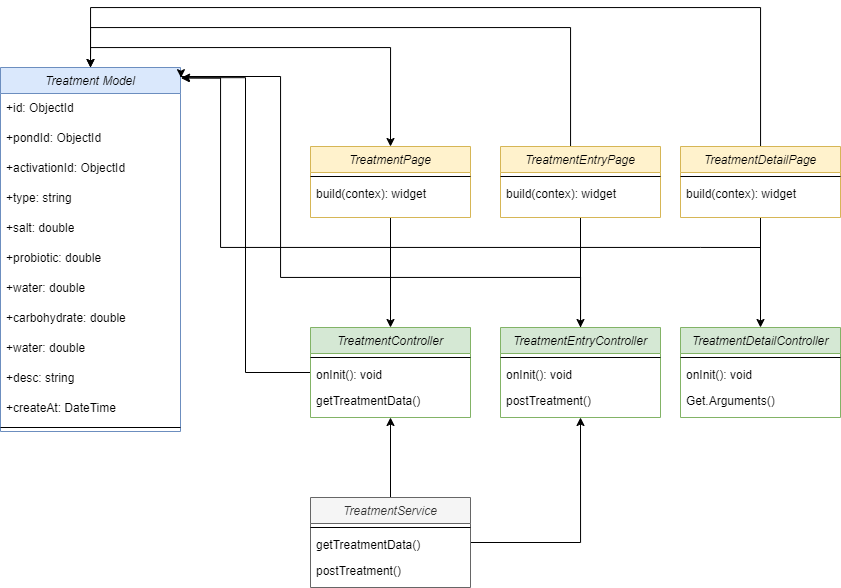
\includegraphics[keepaspectratio, width=6cm]{gambar/treatmentcd}
	 \caption{\textit{Class Diagram Fitur Sprint-6}}
	 \label{gambar:treatmentcd}
	 \end{figure}

	\item{\textit{Menerapkan Mockup-UI Fitur Treatment Kolam kedalam code flutter}}
	
	Setelah \textit{mock-up UI fitur treatment kolam}, akan dilakukan pengimplementasian \textit{mock-up UI} ke dalam aplikasi menggukan flutter. Pada lampiran 7 terdapat source code dari implementasi fitur treatment yang dikelompokan berdasarkan halaman yang menghasilkan halaman seperti dibawah ini.
	
	\begin{figure}[H]
		\centering
		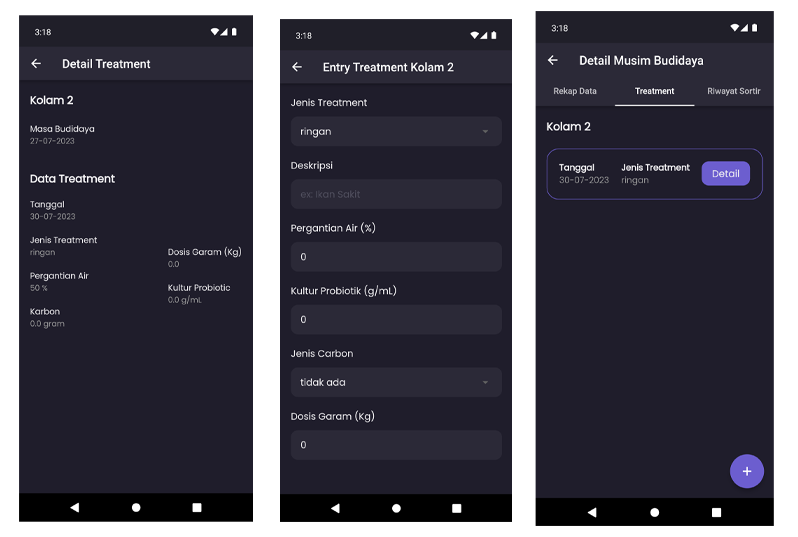
\includegraphics[keepaspectratio, width=8cm]{gambar/sssprint6}
		\caption{\textit{Output dari code pada sprint 6}}
		\label{gambar:sssprint6}
		\end{figure}

  \item{Analisis \textit{User Experience}} 
 
  Pada halaman entry treatment, pembudidaya harus memasukan data yang diperlukan untuk melakukan treatment kolam sesuai dengan kesepakatan saat meeting. Selain itu terdapat juga list mengenai data treatment yang telah dimasukan yang berisi informasi yang berhubungan dengan treatment kolam. Terdapat pula halaman detail treatment yang berisi informasi yang lebih detail terkait treatment yang telah dilakukan.

\item{Sprint 6 Review dan Sprint 7 Planning}

Sprint 6 diakhiri dengan melakukan weekly meeting pada hari selasa dengan agenda melakukan review dan testing terkait hasil sprint 6 dan melakukan planning untuk sprint 7 dengan rincian:
\begin{enumerate}
	\item{\textit{Review dan Testing hasil dari sprint 6}}

	Telah dilakukan review dan testing oleh penulis selaku developer dengan Scrum Master. Setelah dilakukan testing, Scrum Master menyimpulkan bahwa fitur treatment kolam telah berjalan dengan baik.

	\item{\textit{Sprint Planning untuk Sprint 7}}
	
	Planning untuk sprint 7 yakni membuat halaman untuk fitur treatment kolam pada aplikasi \textit{Assistive Aquaculture Breeding Management}.
\end{enumerate}
\end{enumerate}
%!TEX root = ./template-skripsi.tex

\subsection{\textit{Sprint 8}}

	\textit{Sprint-8} dilakukan sepekan pada tanggal 4 oktober 2022 sampai dengan 11 oktober 2022. \textit{Story} ketujuh pada \textit{product backlog} yaitu mengintegrasikan fitur treatment kolam dipecah menjadi beberapa \textit{task} sebagai berikut.


 \begin{longtable}[c]{@{} |p{1cm}|p{4cm}|p{5cm}|p{3cm}| @{}}
 \caption{\textit{Sprint 7} \label{sprint7_table}}\\


 \hline
  \multirow{1}{=}{\centering{\textbf{No}}} & \multirow{1}{=}{\centering{\textbf{\textit{Story}}}} & \multirow{1}{=}{\centering{\textbf{\textit{Task}}}} & \multirow{1}{=}{\centering{\textbf{\textit{Status}}}}\\
 \endfirsthead

 \hline
  \multirow{1}{=}{\centering{\textbf{No}}} & \multirow{1}{=}{\centering{\textbf{\textit{Story}}}} & \multirow{1}{=}{\centering{\textbf{\textit{Task}}}} & \multirow{1}{=}{\centering{\textbf{\textit{Status}}}}\\
 \endhead

 \hline
 \endfoot

 \hline
 \endlastfoot

 \hline
 1 & Mengitegrasikan fitur treatment kolam dengan webservice &  Mengitegrasikan fitur treatment kolam dengan webservice &  selesai \\
 \hline
 \end{longtable}

Pada sprint ketujuh ini story yang di pilih untuk di uraikan pada sprint kali ini adalah membuat halaman rekapitulasi treatment kolam, entry treatment kolam. Tujuan dari \textit{sprint-7} ini adalah membuat fitur rekapitulasi treatment kolam dan mengintegrasikan halaman tersebut dengan webservice yang sudah dibuat oleh penelitian Andri Rahmanto.

\begin{enumerate}[listparindent=2em]
	
	\item{\textit{Mengitegrasikan fitur treatment kolam dengan webservice}}

	Sebelumnya pada sprint keenam, setiap data pada fitur treatment masih berupa data dummy sehingga perlu diintegrasikan dengan webservice agar aplikasi dapat berjalan dengan data yang asli. Hal yang dilakukan dalam mengintegrasikan fitur treatment dengan webservice terdapat pada lampiran 8.
	

\item{Sprint 7 Review dan Sprint 8 Planning}

Sprint 7 diakhiri dengan melakukan weekly meeting pada hari selasa dengan agenda melakukan review dan testing terkait hasil sprint 7 dan melakukan planning untuk sprint 8 dengan rincian:
\begin{enumerate}
	\item{\textit{Review dan Testing hasil dari sprint 8}}

	Telah dilakukan review dan testing oleh penulis selaku developer dengan Scrum Master. Setelah dilakukan testing, Scrum Master menyimpulkan bahwa fitur treatment kolam telah berjalan dengan baik.

  \begin{longtable}{| p{8cm} | c | c | l |}
    \caption{Unit testing Halaman Rekapitulasi Treatment.\label{table:unit_testing_rekapitulasi_treatment}}\\
    \hline
    \multirow{2}{*}{Skenario Pengujian} & \multicolumn{2}{l|}{Kesesuaian} & \multirow{2}{*}{Kesimpulan} \\ 
    \cline{2-3}
      & \multicolumn{1}{l|}{sesuai} & tidak sesuai & \\ 
    \hline
    \hline
    \endfirsthead
    \hline
    \multirow{2}{*}{Skenario Pengujian} & \multicolumn{2}{l|}{Kesesuaian} & \multirow{2}{*}{Kesimpulan} \\ 
    \cline{2-3}
      & \multicolumn{1}{l|}{sesuai} & tidak sesuai &  \\ 
    \hline
    \hline
    \endhead
    \hline
    \endfoot
    
    
    \hline\hline
    \endlastfoot
    Ketika menekan list data treatment, maka akan ditamplikan detail treatment & \Checkmark &  & Diterima \\ 
    \hline
    Saat ikon (+) ditekan maka akan menampilkan halaman entry treatment & \Checkmark &  & Diterima \\ 
    \hline
    ketika mengisi form treatment dengan data yang sesuai dan menekan submit, data treatment akan ditambahkan & \Checkmark &  & Diterima \\ 
    \hline
    \end{longtable}    

	\item{\textit{Sprint Planning untuk Sprint 8}}
	
	Planning untuk sprint 8 yakni membuat fitur pencatatan kualitas air harian pada aplikasi \textit{Assistive Aquaculture Breeding Management}.
\end{enumerate}
\end{enumerate}
%!TEX root = ./template-skripsi.tex

\subsection{\textit{Sprint 8}}

	\textit{Sprint-8} dilakukan sepekan pada tanggal 11 oktober 2022 sampai dengan 18 oktober 2022. \textit{Story} kedelapan pada \textit{product backlog} yaitu membuat fitur pencatatan kualitas air harian dipecah menjadi beberapa \textit{task} sebagai berikut.


 \begin{longtable}[c]{@{} |p{1cm}|p{4cm}|p{5cm}|p{3cm}| @{}}
 \caption{\textit{Sprint 8} \label{sprint8_table}}\\


 \hline
  \multirow{1}{=}{\centering{\textbf{No}}} & \multirow{1}{=}{\centering{\textbf{\textit{Story}}}} & \multirow{1}{=}{\centering{\textbf{\textit{Task}}}} & \multirow{1}{=}{\centering{\textbf{\textit{Status}}}}\\
 \endfirsthead

 \hline
  \multirow{1}{=}{\centering{\textbf{No}}} & \multirow{1}{=}{\centering{\textbf{\textit{Story}}}} & \multirow{1}{=}{\centering{\textbf{\textit{Task}}}} & \multirow{1}{=}{\centering{\textbf{\textit{Status}}}}\\
 \endhead

 \hline
 \endfoot

 \hline
 \endlastfoot

 \hline
 1 & Membuat fitur pencatatan kualitas air harian &  Membuat \textit{Mock-up UI} halaman list pencatatan kualitas air harian, entry kualitas air harian, detail kualitas air harian  &  selesai \\
 \hline
 2 & & Menerapkan \textit{Mock-up UI} halaman list pencatatan kualitas air harian, entry kualitas air harian, detail kualitas air harian ke Flutter & selesai\\
 \hline
 3 & & Mengintegrasikan halaman pencatatan kualitas air harian, entry kualitas air harian, detail kualitas air harian ke \textit{webservice} & selesai\\
 \hline
 \end{longtable}

Pada sprint kedelapan ini story yang di pilih untuk di uraikan pada sprint kali ini adalah membuat halaman pencatatan kualitas air harian, entry kualitas air harian, detail kualitas air harian. Tujuan dari \textit{sprint-8} ini adalah membuat fitur pencatatan kualitas air harian dan mengintegrasikan halaman tersebut dengan webservice yang sudah dibuat oleh penelitian Andri Rahmanto.

\begin{enumerate}[listparindent=2em]
	
	\item{\textit{Membuat Mock-up UI Fitur Pencatatan Kualitas Air Harian}}
	
	Pembuatan konten dan fitur yang terdapat pada \textit{mock-up UI} fitur pencatatan kualitas air harian dilakukan berdasarkan persetujuan product owner dan scrum master pada meeting sebelumnya. Mock-up UI dibuat menggunakan platform figma.
	
	\begin{figure}[H]
	\centering
	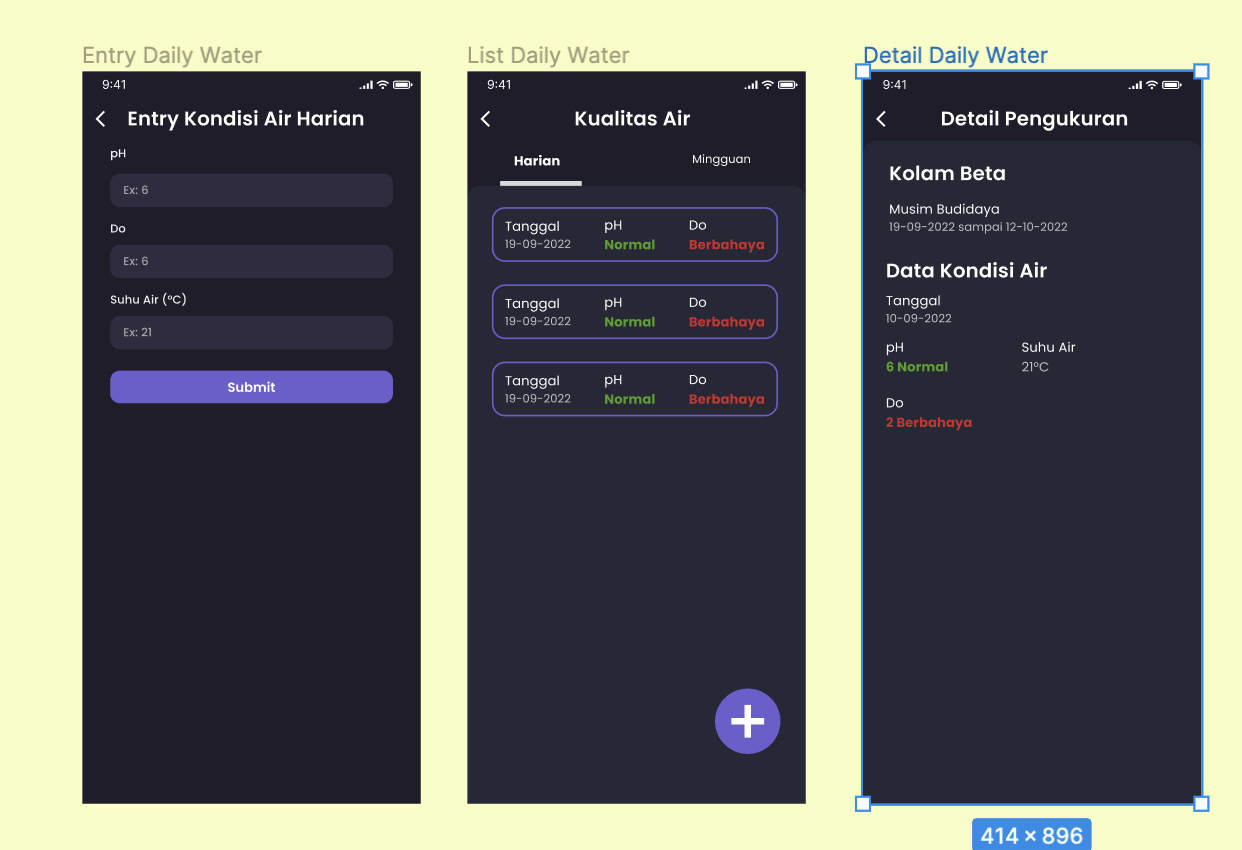
\includegraphics[keepaspectratio, width=6cm]{gambar/mockupairharian}
	\caption{\textit{Mock-up UI Fitur Pencatatan Kualitas Air Harian}}
	\label{gambar:mockupairharian}
	\end{figure}

	\item{\textit{Class Diagram}}
	
	Class Diagram menggambarkan kelas-kelas yang akan dipakai oleh sistem. Umumnya terdapat 3 kelas pada setiap module yaitu class model, controller, dan view. Pada sprint-8 penelitian kali ini penulis membuat 4 class yaitu model yang berwarna biru, view berwarna oranye, controller yang berwarna hijau, dan service yang berwarna kuning.
	 
	 \begin{figure}[H]
	 \centering
	 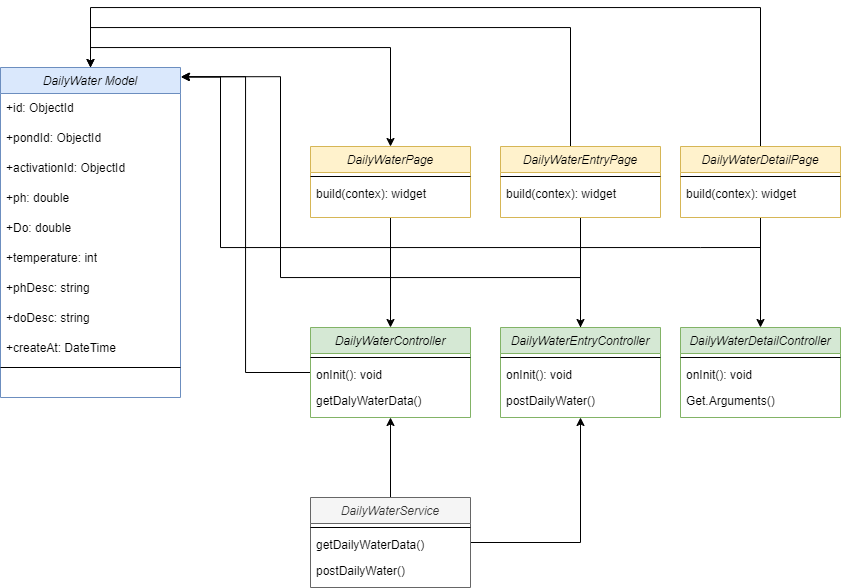
\includegraphics[keepaspectratio, width=6cm]{gambar/dailycd}
	 \caption{\textit{Class Diagram Fitur Sprint-8}}
	 \label{gambar:dailycd}
	 \end{figure}

	\item{\textit{Menerapkan Mockup-UI Fitur Pencatatan Kualitas Air Harian kedalam code flutter}}
	
	Setelah itu, akan dilakukan pengimplementasian \textit{mock-up UI} ke dalam aplikasi menggukan flutter. Pada lampiran 9 terdapat source code dari implementasi fitur pencatatan kualitas air harian yang dikelompokan berdasarkan halaman yang menghasilkan output halaman sebagai seperti dibawah ini.

	\begin{figure}[H]
		\centering
		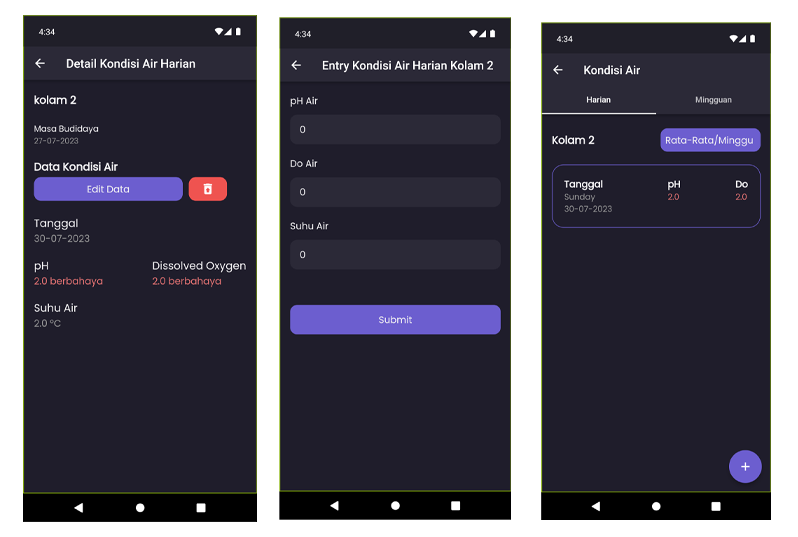
\includegraphics[keepaspectratio, width=8cm]{gambar/sssprint8}
		\caption{\textit{Output dari code pada sprint 8}}
		\label{gambar:sssprint8}
		\end{figure}

	\item{\textit{Mengitegrasikan fitur pencatatan kualitas air harian dengan webservice}}

	Sebelumnya, setiap data pada fitur masih berupa data dummy sehingga perlu diintegrasikan dengan webservice agar aplikasi dapat berjalan dengan data yang asli. Hal yang dilakukan dalam mengintegrasikan fitur pencatatan kualitas air harian dengan webservice terdapat pada lampiran 9.

  \item{Analisis \textit{User Experience}} 
 
  Pada halaman entry daily water quality, pembudidaya harus memasukan data yang diperlukan untuk melakukan daily water quality sesuai dengan kesepakatan saat meeting, seperti pH, Dissolved Oxygen, dan suhu. Selain itu terdapat juga list mengenai data daily water quality yang telah dimasukan yang berisi informasi yang berhubungan dengan daily water quality. Terdapat pula halaman detail daily water quality yang berisi informasi yang lebih detail terkait daily water quality yang telah dilakukan.

\item{Sprint 8 Review dan Sprint 9 Planning}

Sprint 8 diakhiri dengan melakukan weekly meeting pada hari selasa dengan agenda melakukan review dan testing terkait hasil sprint 8 dan melakukan planning untuk sprint 9 dengan rincian:
\begin{enumerate}
	\item{\textit{Review dan Testing hasil dari sprint 8}}

	Telah dilakukan review dan testing oleh penulis selaku developer dengan Scrum Master. Setelah dilakukan testing, Scrum Master menyimpulkan bahwa fitur pencatatan kualitas air harian telah berjalan dengan baik.

	\item{\textit{Sprint Planning untuk Sprint 9}}
	
	Planning untuk sprint 9 yakni membuat fitur pencatatan kualitas air mingguan pada aplikasi \textit{Assistive Aquaculture Breeding Management}.
\end{enumerate}
\end{enumerate}
%!TEX root = ./template-skripsi.tex

\subsection{\textit{Sprint 9}}

	\textit{Sprint-9} dilakukan sepekan pada tanggal 18 oktober 2022 sampai dengan 25 oktober 2022. \textit{Story} kesembilan pada \textit{product backlog} yaitu membuat fitur pencatatan kualitas air mingguan dipecah menjadi beberapa \textit{task} sebagai berikut.


 \begin{longtable}[c]{@{} |p{1cm}|p{4cm}|p{5cm}|p{3cm}| @{}}
 \caption{\textit{Sprint 9} \label{sprint9_table}}\\


 \hline
  \multirow{1}{=}{\centering{\textbf{No}}} & \multirow{1}{=}{\centering{\textbf{\textit{Story}}}} & \multirow{1}{=}{\centering{\textbf{\textit{Task}}}} & \multirow{1}{=}{\centering{\textbf{\textit{Status}}}}\\
 \endfirsthead

 \hline
  \multirow{1}{=}{\centering{\textbf{No}}} & \multirow{1}{=}{\centering{\textbf{\textit{Story}}}} & \multirow{1}{=}{\centering{\textbf{\textit{Task}}}} & \multirow{1}{=}{\centering{\textbf{\textit{Status}}}}\\
 \endhead

 \hline
 \endfoot

 \hline
 \endlastfoot

 \hline
 1 & Membuat fitur pencatatan kualitas air mingguan &  Membuat \textit{Mock-up UI} halaman list pencatatan kualitas air mingguan, entry kualitas air mingguan, detail kualitas air mingguan  &  selesai \\
 \hline
 2 & & Menerapkan \textit{Mock-up UI} halaman list pencatatan kualitas air mingguan, entry kualitas air mingguan, detail kualitas air mingguan ke Flutter & selesai\\
 \hline
 3 & & Mengintegrasikan halaman pencatatan kualitas air mingguan, entry kualitas air mingguan, detail kualitas air mingguan ke \textit{webservice} & selesai\\
 \hline
 \end{longtable}

Pada sprint kesembilan ini story yang di pilih untuk di uraikan pada sprint kali ini adalah membuat halaman pencatatan kualitas air mingguan, entry kualitas air mingguan, detail kualitas air mingguan. Tujuan dari \textit{sprint-9} ini adalah membuat fitur pencatatan kualitas air mingguan dan mengintegrasikan halaman tersebut dengan webservice yang sudah dibuat oleh penelitian Andri Rahmanto.

\begin{enumerate}[listparindent=2em]
	
	\item{\textit{Membuat Mock-up UI Fitur Pencatatan Kualitas air mingguan}}
	
	Pembuatan konten dan fitur yang terdapat pada \textit{mock-up UI} fitur pencatatan kualitas air mingguan dilakukan berdasarkan persetujuan product owner dan scrum master pada meeting sebelumnya. Mock-up UI dibuat menggunakan platform figma.
	
	\begin{figure}[H]
	\centering
	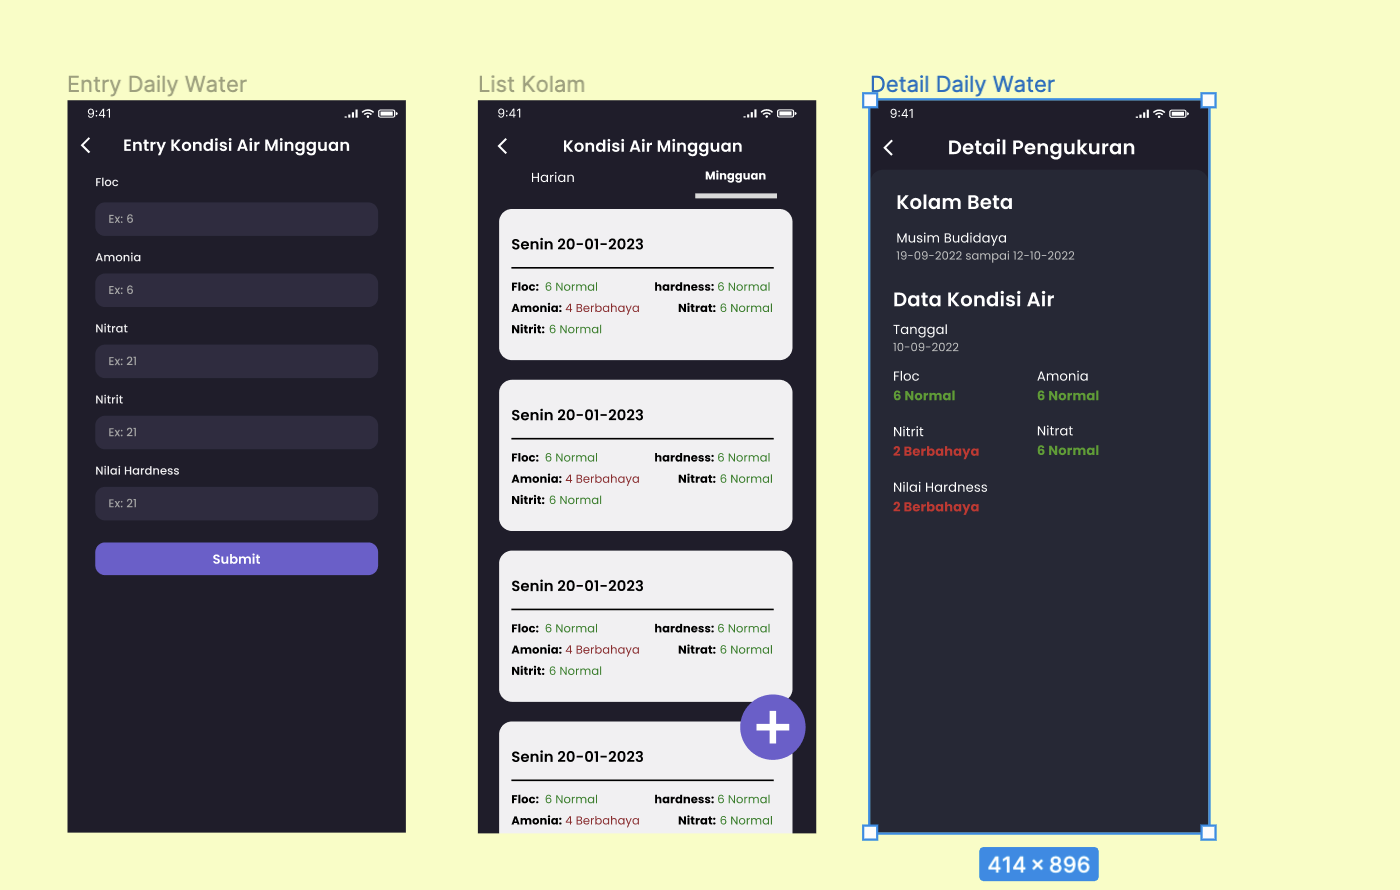
\includegraphics[keepaspectratio, width=6cm]{gambar/mockupairmingguan}
	\caption{\textit{Mock-up UI Fitur Pencatatan Kualitas air mingguan}}
	\label{gambar:mockupairmingguan}
	\end{figure}

	\item{\textit{Class Diagram}}
	
	Class Diagram menggambarkan kelas-kelas yang akan dipakai oleh sistem. Umumnya terdapat 3 kelas pada setiap module yaitu class model, controller, dan view. Pada sprint-9 penelitian kali ini penulis membuat 4 class yaitu model yang berwarna biru, view berwarna oranye, controller yang berwarna hijau, dan service yang berwarna kuning.
	 
	 \begin{figure}[H]
	 \centering
	 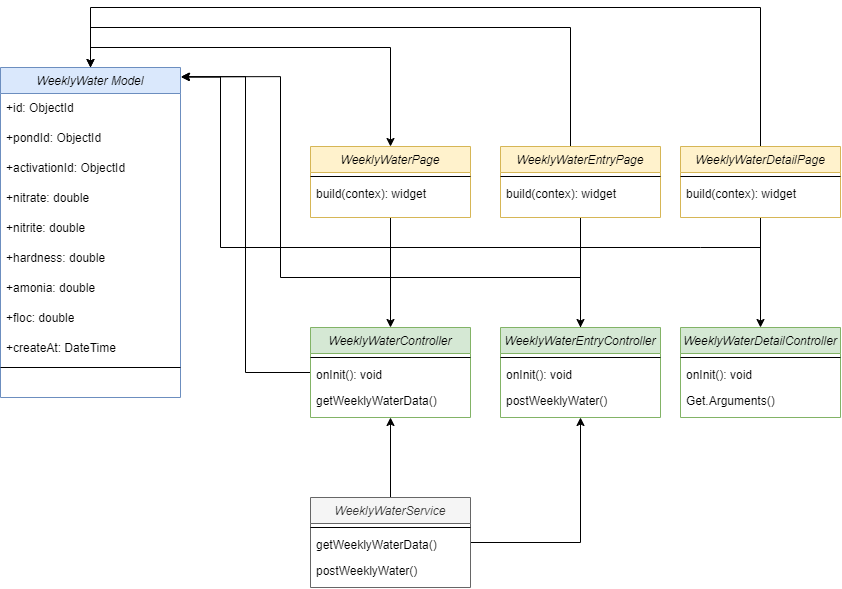
\includegraphics[keepaspectratio, width=6cm]{gambar/weeklycd}
	 \caption{\textit{Class Diagram Fitur Sprint-9}}
	 \label{gambar:weeklycd}
	 \end{figure}

	\item{\textit{Menerapkan Mockup-UI Fitur Pencatatan Kualitas air mingguan kedalam code flutter}}
	
	Setelah itu, akan dilakukan pengimplementasian \textit{mock-up UI} ke dalam aplikasi menggukan flutter. Pada lampiran 10 terdapat source code dari implementasi fitur pencatatan kualitas air mingguan yang dikelompokan berdasarkan halaman yang menghasilkan output halaman seperti dibawah ini

	\begin{figure}[H]
		\centering
		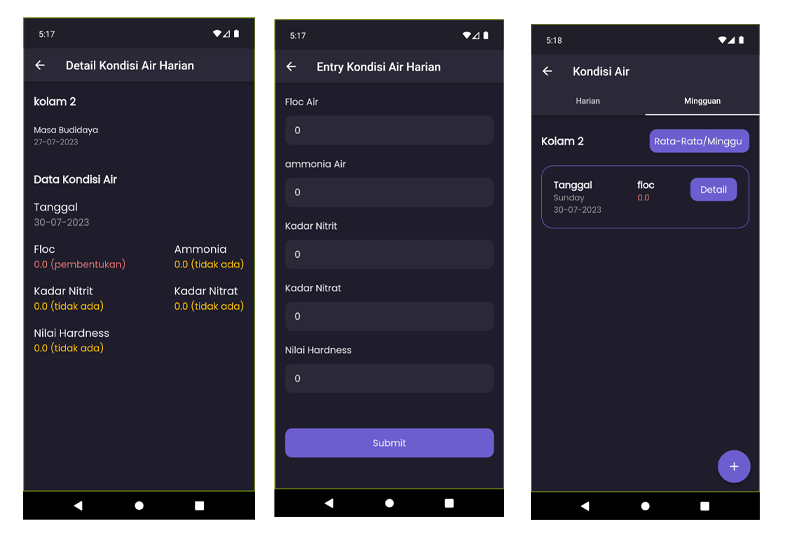
\includegraphics[keepaspectratio, width=8cm]{gambar/sssprint9}
		\caption{\textit{Output dari code pada sprint 9}}
		\label{gambar:sssprint9}
		\end{figure}

	\item{\textit{Mengitegrasikan fitur pencatatan kualitas air mingguan dengan webservice}}

	Sebelumnya, setiap data pada fitur masih berupa data dummy sehingga perlu diintegrasikan dengan webservice agar aplikasi dapat berjalan dengan data yang asli. Hal yang dilakukan dalam mengintegrasikan fitur pencatatan kualitas air mingguan dengan webservice terdapat pada lampiran 10.

  \item{Analisis \textit{User Experience}} 
 
  Pada halaman entry weekly water quality, pembudidaya harus memasukan data yang diperlukan untuk melakukan weekly water quality sesuai dengan kesepakatan saat meeting, seperti kadar nitrit, nitrat, amonia, dan nilai kekerasan air. Selain itu terdapat juga list mengenai data weekly water quality yang telah dimasukan yang berisi informasi yang berhubungan dengan weekly water quality. Terdapat pula halaman detail weekly water quality yang berisi informasi yang lebih detail terkait weekly water quality yang telah dilakukan.

\item{Sprint 9 Review dan Sprint 10 Planning}

Sprint 9 diakhiri dengan melakukan weekly meeting pada hari selasa dengan agenda melakukan review dan testing terkait hasil sprint 9 dan melakukan planning untuk sprint 10 dengan rincian:
\begin{enumerate}
	\item{\textit{Review dan Testing hasil dari sprint 9}}

	Telah dilakukan review dan testing oleh penulis selaku developer dengan Scrum Master. Setelah dilakukan testing, Scrum Master menyimpulkan bahwa fitur pencatatan kualitas air mingguan telah berjalan dengan baik.
	
  \begin{longtable}{| p{8cm} | c | c | l |}
    \caption{Unit testing Halaman Kualitas Air.\label{table:unit_testing_fitur_kualitas_air}}\\
    \hline
    \multirow{2}{*}{Skenario Pengujian} & \multicolumn{2}{l|}{Kesesuaian} & \multirow{2}{*}{Kesimpulan} \\ 
    \cline{2-3}
      & \multicolumn{1}{l|}{sesuai} & tidak sesuai & \\ 
    \hline
    \hline
    \endfirsthead
    \hline
    \multirow{2}{*}{Skenario Pengujian} & \multicolumn{2}{l|}{Kesesuaian} & \multirow{2}{*}{Kesimpulan} \\ 
    \cline{2-3}
      & \multicolumn{1}{l|}{sesuai} & tidak sesuai &  \\ 
    \hline
    \hline
    \endhead
    \hline
    \endfoot
    
    
    \hline\hline
    \endlastfoot
    Ketika memilih musim budidaya dan maka akan ditampilkan list pengontrolan kualitas air kolam & \Checkmark &  & Diterima \\ 
    \hline
    Ketika menekan list data pengontrolan kualitas air, maka akan ditamplikan detail pengontrolan kualitas air kolam & \Checkmark &  & Diterima \\ 
    \hline
    Saat ikon (+) ditekan maka akan menampilkan halaman entry pengontrolan kualitas air kolam & \Checkmark &  & Diterima \\ 
    \hline
    ketika mengisi form pengontrolan kualitas air kolam dengan data yang sesuai dan menekan submit, data pengontrolan kualitas air akan ditambahkan & \Checkmark &  & Diterima \\ 
    \hline
    \end{longtable}

	\item{\textit{Sprint Planning untuk Sprint 10}}
	
	Planning untuk sprint 10 yakni membuat fitur sortir kolam mingguan pada aplikasi \textit{Assistive Aquaculture Breeding Management}.
\end{enumerate}
\end{enumerate}
%!TEX root = ./template-skripsi.tex

\subsection{\textit{Sprint 10}}

	\textit{Sprint-10} dilakukan sepekan pada tanggal 25 oktober 2022 sampai dengan 1 november 2022. \textit{Story} kesepuluh pada \textit{product backlog} yaitu membuat fitur perpindahan antar kolam dipecah menjadi beberapa \textit{task} sebagai berikut.


 \begin{longtable}[c]{@{} |p{1cm}|p{4cm}|p{5cm}|p{3cm}| @{}}
 \caption{\textit{Sprint 10} \label{sprint10_table}}\\


 \hline
  \multirow{1}{=}{\centering{\textbf{No}}} & \multirow{1}{=}{\centering{\textbf{\textit{Story}}}} & \multirow{1}{=}{\centering{\textbf{\textit{Task}}}} & \multirow{1}{=}{\centering{\textbf{\textit{Status}}}}\\
 \endfirsthead

 \hline
  \multirow{1}{=}{\centering{\textbf{No}}} & \multirow{1}{=}{\centering{\textbf{\textit{Story}}}} & \multirow{1}{=}{\centering{\textbf{\textit{Task}}}} & \multirow{1}{=}{\centering{\textbf{\textit{Status}}}}\\
 \endhead

 \hline
 \endfoot

 \hline
 \endlastfoot

 \hline
 1 & Membuat fitur sortir kolam &  Membuat \textit{Mock-up UI} halaman list sortir, detail sortir, entry sortir &  selesai \\
 \hline
 2 & & Menerapkan \textit{Mock-up UI} halaman list sortir, detail sortir, entry sortir  ke Flutter & selesai\\
 \hline
 3 & & Mengintegrasikan halaman list soritr, entry soritr, detail soritr ke \textit{webservice} & selesai\\
 \hline
 \end{longtable}

Pada sprint kesepuluh ini story yang di pilih untuk di uraikan pada sprint kali ini adalah membuat fitur sortir. Tujuan dari \textit{sprint-10} ini adalah membuat fitur sortir ikan dan mengintegrasikan halaman tersebut dengan webservice yang sudah dibuat oleh penelitian Andri Rahmanto.

\begin{enumerate}[listparindent=2em]
	
	\item{\textit{Membuat Mock-up UI Fitur Sortir Kolam}}
	
	Pembuatan konten dan fitur yang terdapat pada \textit{mock-up UI} fitur sortir kolam dilakukan berdasarkan persetujuan product owner dan scrum master pada meeting sebelumnya. Mock-up UI dibuat menggunakan platform figma.
	
	\begin{figure}[H]
	\centering
	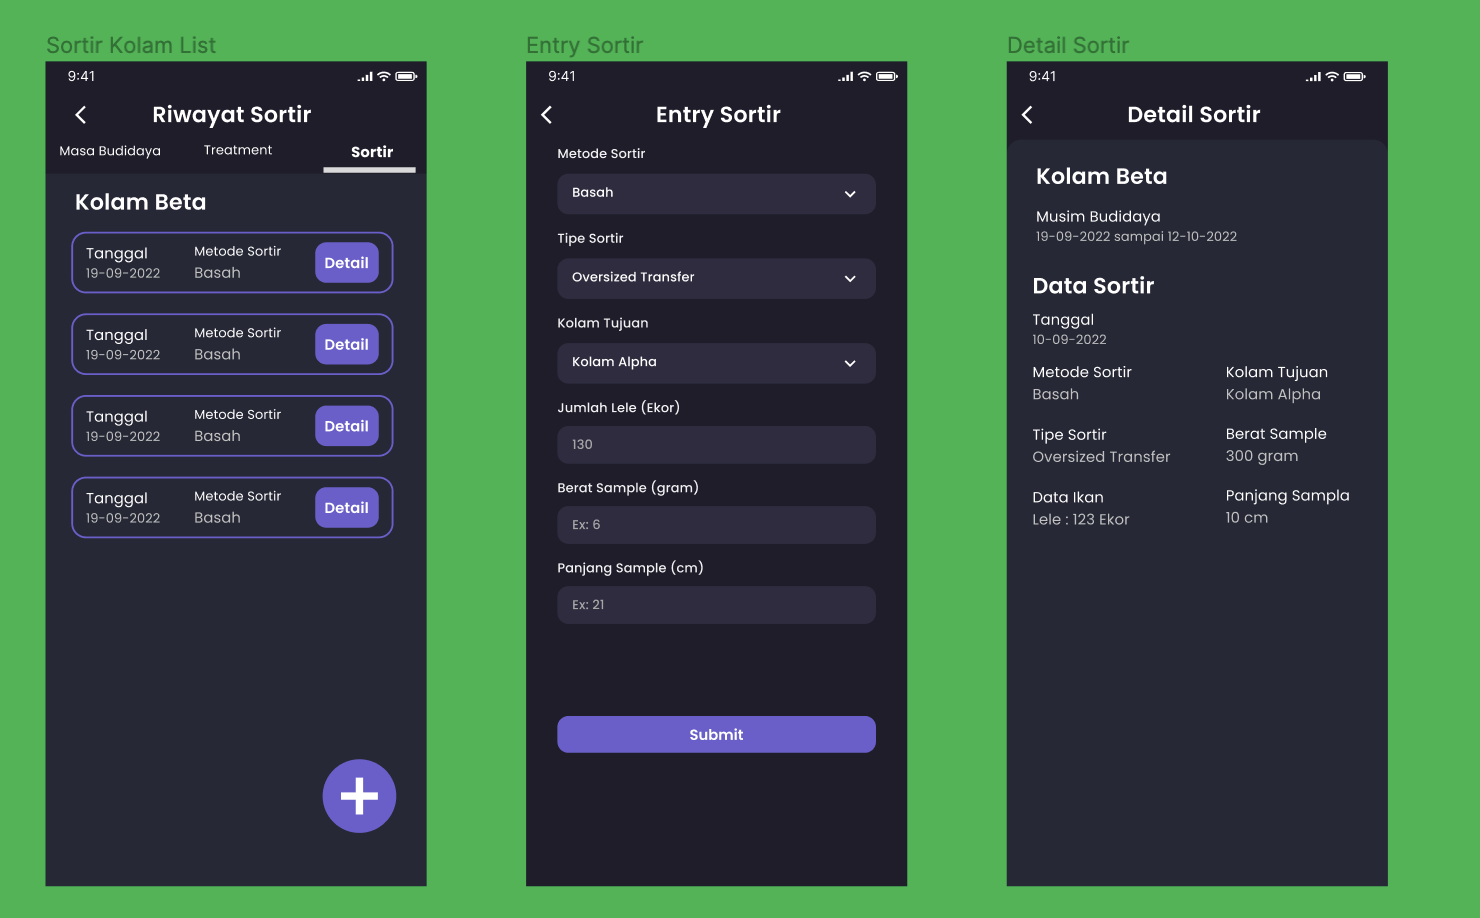
\includegraphics[keepaspectratio, width=10cm]{gambar/mockupsortir}
	\caption{\textit{Mock-up UI Fitur Sortir}}
	\label{gambar:mockupsortir}
	\end{figure}

	\item{\textit{Class Diagram}}
	
	Class Diagram menggambarkan kelas-kelas yang akan dipakai oleh sistem. Umumnya terdapat 3 kelas pada setiap module yaitu class model, controller, dan view. Pada sprint-10 penelitian kali ini penulis membuat 4 class yaitu model yang berwarna biru, view berwarna oranye, controller yang berwarna hijau, dan service yang berwarna kuning.
	 
	 \begin{figure}[H]
	 \centering
	 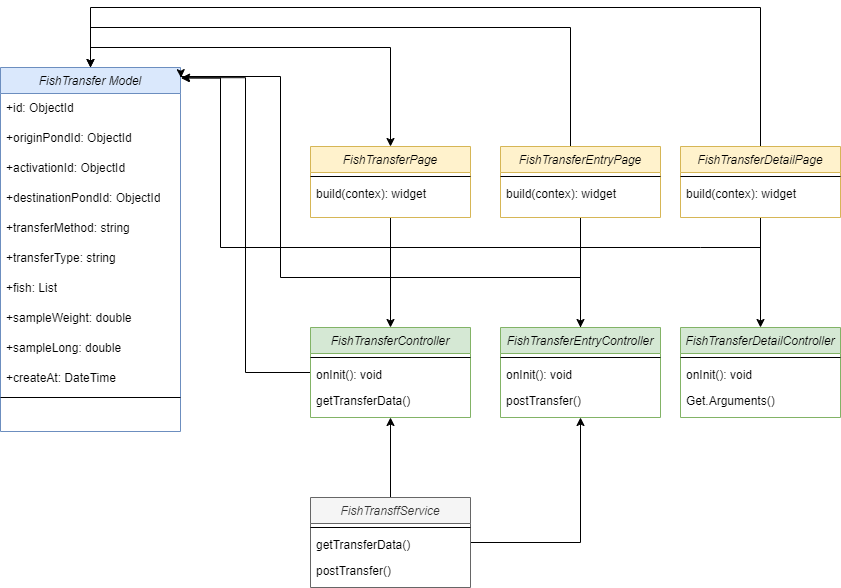
\includegraphics[keepaspectratio, width=6cm]{gambar/transfercd}
	 \caption{\textit{Class Diagram Fitur Sprint-10}}
	 \label{gambar:transfercd}
	 \end{figure}

	\item{\textit{Menerapkan Mockup-UI Fitur Sortir Kolam kedalam code flutter}}
	
	Setelah \textit{mock-up UI fitur Sortir kolam}, akan dilakukan pengimplementasian \textit{mock-up UI} ke dalam aplikasi menggukan flutter. Pada lampiran 11 terdapat source code dari implementasi fitur sortir yang dikelompokan berdasarkan halaman yang menghasilkan output halaman seperti dibawah ini.

	\begin{figure}[H]
		\centering
		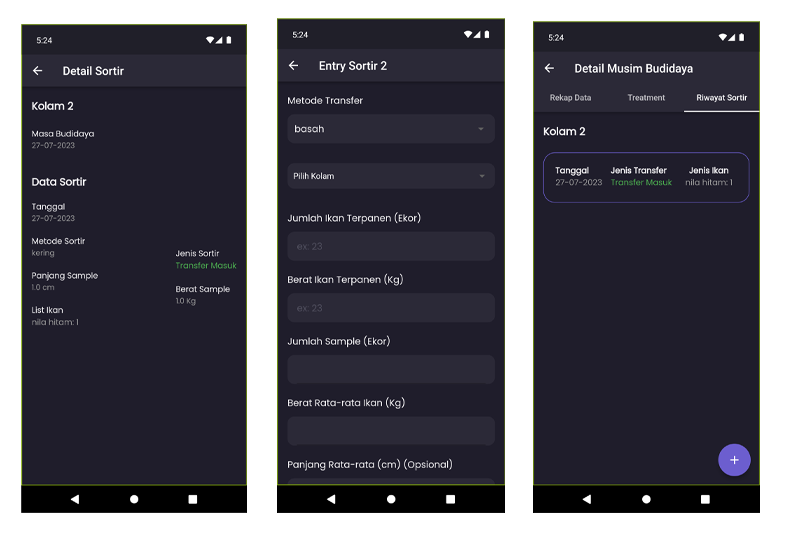
\includegraphics[keepaspectratio, width=8cm]{gambar/sssprint10}
		\caption{\textit{Output dari code pada sprint 10}}
		\label{gambar:sssprint10}
		\end{figure}

    \item{\textit{Mengitegrasikan fitur pencatatan kualitas air mingguan dengan webservice}}

	Sebelumnya, setiap data pada fitur masih berupa data dummy sehingga perlu diintegrasikan dengan webservice agar aplikasi dapat berjalan dengan data yang asli. Hal yang dilakukan dalam mengintegrasikan fitur sortir ikan dengan webservice terdapat pada lampiran 11.

  \item{Analisis \textit{User Experience}} 
 
  Pada halaman entry sortir kolam/transfer ikan, pembudidaya harus memasukan data yang diperlukan untuk melakukan sortir kolam/transfer ikan sesuai dengan kesepakatan saat meeting. Selain itu terdapat juga list mengenai data sortir kolam/transfer ikan yang telah dimasukan yang berisi informasi yang berhubungan dengan sortir kolam/transfer ikan. Terdapat pula halaman detail sortir kolam/transfer ikan yang berisi informasi yang lebih detail terkait sortir kolam/transfer ikan yang telah dilakukan.

\item{Sprint 10 Review dan Sprint 11 Planning}

Sprint 10 diakhiri dengan melakukan weekly meeting pada hari selasa dengan agenda melakukan review dan testing terkait hasil sprint 10 dan melakukan planning untuk sprint 11 dengan rincian:
\begin{enumerate}
	\item{\textit{Review dan Testing hasil dari sprint 10}}

	Telah dilakukan review dan testing oleh penulis selaku developer dengan Scrum Master. Setelah dilakukan testing, Scrum Master menyimpulkan bahwa fitur transfer/sortir ikam telah berjalan dengan baik.
	
  \begin{longtable}{| p{8cm} | c | c | l |}
    \caption{Unit testing Halaman Rekapitulasi Sortir.\label{table:unit_testing_rekapitulasi_sortir}}\\
    \hline
    \multirow{2}{*}{Skenario Pengujian} & \multicolumn{2}{l|}{Kesesuaian} & \multirow{2}{*}{Kesimpulan} \\ 
    \cline{2-3}
      & \multicolumn{1}{l|}{sesuai} & tidak sesuai & \\ 
    \hline
    \hline
    \endfirsthead
    \hline
    \multirow{2}{*}{Skenario Pengujian} & \multicolumn{2}{l|}{Kesesuaian} & \multirow{2}{*}{Kesimpulan} \\ 
    \cline{2-3}
      & \multicolumn{1}{l|}{sesuai} & tidak sesuai &  \\ 
    \hline
    \hline
    \endhead
    \hline
    \endfoot
    
    
    \hline\hline
    \endlastfoot
    Ketika menekan list data sortir, maka akan ditamplikan detail sortir & \Checkmark &  & Diterima \\ 
    \hline
    Saat ikon (+) ditekan maka akan menampilkan halaman entry sortir & \Checkmark &  & Diterima \\ 
    \hline
    ketika mengisi form sortir dengan data yang sesuai dan menekan submit, data sortir akan ditambahkan & \Checkmark &  & Diterima \\ 
    \hline
    \end{longtable}

	\item{\textit{Sprint Planning untuk Sprint 11}}
	
	Planning untuk sprint 11 yakni membuat fitur multi user pada aplikasi \textit{Assistive Aquaculture Breeding Management}.
\end{enumerate}
\end{enumerate}
%!TEX root = ./template-skripsi.tex

\subsection{\textit{Sprint 11}}

	\textit{Sprint-11} dilakukan sepekan pada tanggal 1 november 2022 sampai dengan 8 november 2022. \textit{Story} kesebelas pada \textit{product backlog} yaitu membuat fitur multiuser/login dan register dipecah menjadi beberapa \textit{task} sebagai berikut.


 \begin{longtable}[c]{@{} |p{1cm}|p{4cm}|p{5cm}|p{3cm}| @{}}
 \caption{\textit{Sprint 11} \label{sprint11_table}}\\


 \hline
  \multirow{1}{=}{\centering{\textbf{No}}} & \multirow{1}{=}{\centering{\textbf{\textit{Story}}}} & \multirow{1}{=}{\centering{\textbf{\textit{Task}}}} & \multirow{1}{=}{\centering{\textbf{\textit{Status}}}}\\
 \endfirsthead

 \hline
  \multirow{1}{=}{\centering{\textbf{No}}} & \multirow{1}{=}{\centering{\textbf{\textit{Story}}}} & \multirow{1}{=}{\centering{\textbf{\textit{Task}}}} & \multirow{1}{=}{\centering{\textbf{\textit{Status}}}}\\
 \endhead

 \hline
 \endfoot

 \hline
 \endlastfoot

 \hline
 1 & Membuat multiuser &  Membuat \textit{Mock-up UI} halaman login dan register &  selesai \\
 \hline
 2 & & Menerapkan \textit{Mock-up UI} halaman login dan register ke Flutter & selesai\\
 \hline
 3 & & Mengintegrasikan halaman login dan register ke \textit{webservice} & selesai\\
 \hline
 \end{longtable}

Pada sprint kesebelas ini story yang di pilih untuk di uraikan pada sprint kali ini adalah membuat login dan register. Tujuan dari \textit{sprint-11} ini adalah membuat multiuser dan mengintegrasikan halaman tersebut dengan webservice yang sudah dibuat oleh penelitian Andri Rahmanto.

\begin{enumerate}[listparindent=2em]
	
	\item{\textit{Membuat Mock-up UI Fitur multiuser}}
	
	Pembuatan konten dan fitur yang terdapat pada \textit{mock-up UI} fitur multiuser dilakukan berdasarkan persetujuan product owner dan scrum master pada meeting sebelumnya. Mock-up UI dibuat menggunakan platform figma.
	
	\begin{figure}[H]
	\centering
	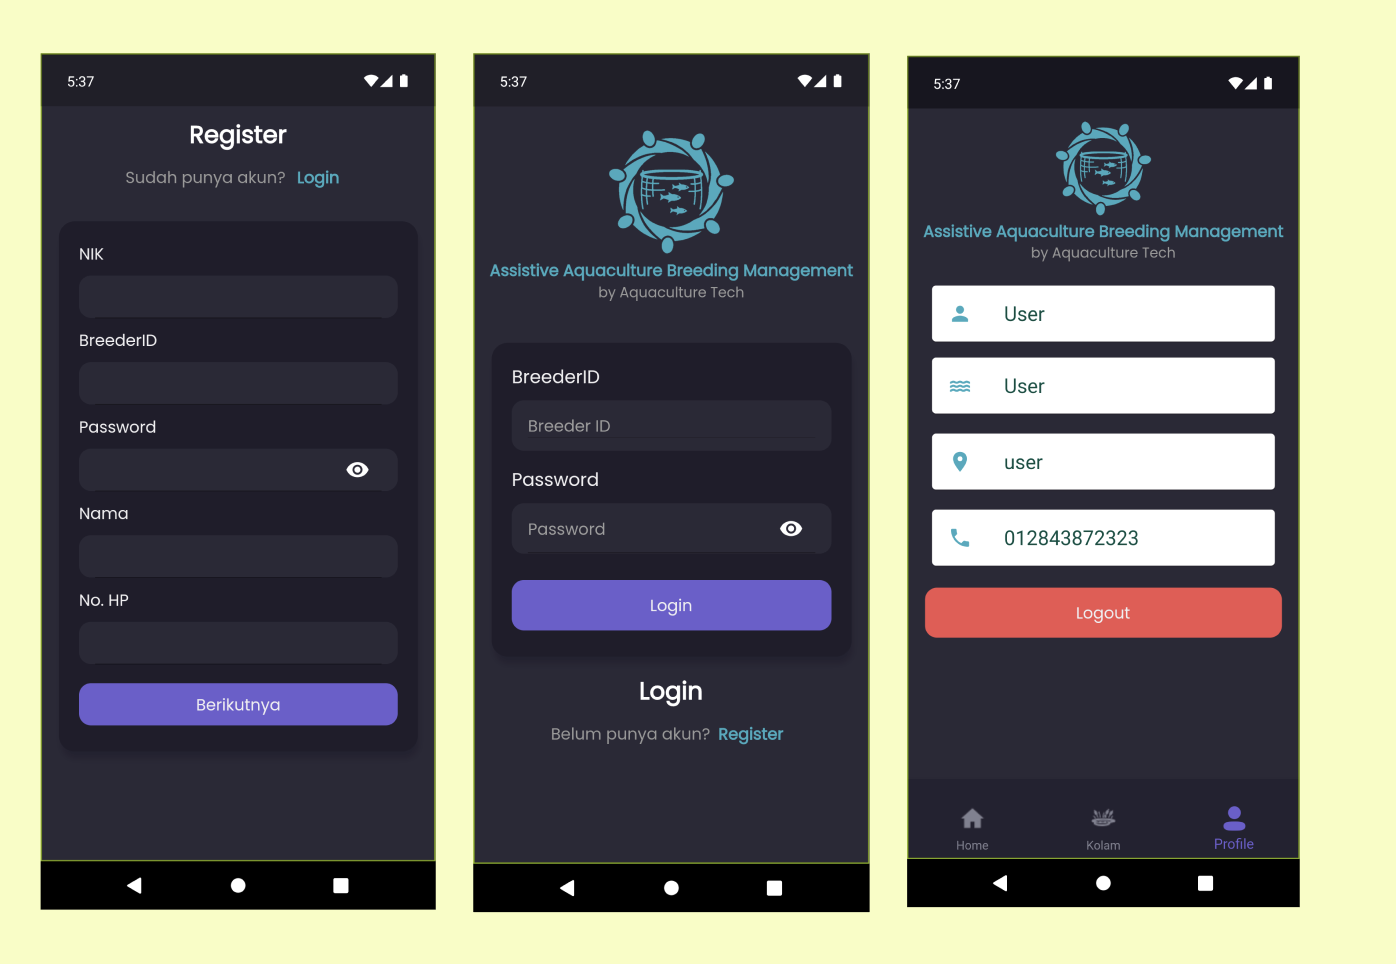
\includegraphics[keepaspectratio, width=6cm]{gambar/mockupmultiuser}
	\caption{\textit{Mock-up UI Fitur multiuser}}
	\label{gambar:mockupmultiuser}
	\end{figure}

	\item{\textit{Class Diagram}}
	
	Class Diagram menggambarkan kelas-kelas yang akan dipakai oleh sistem. Umumnya terdapat 3 kelas pada setiap module yaitu class model, controller, dan view. Pada sprint-11 penelitian kali ini penulis membuat 4 class yaitu model yang berwarna biru, view berwarna oranye, controller yang berwarna hijau, dan service yang berwarna kuning.
	 
	 \begin{figure}[H]
	 \centering
	 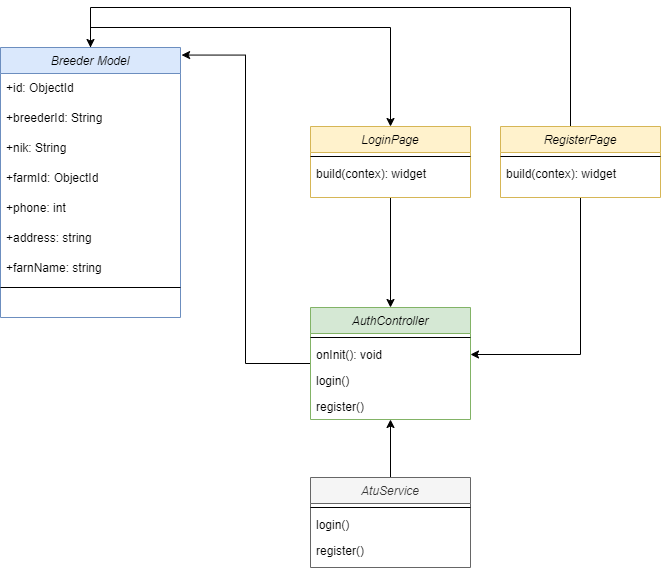
\includegraphics[keepaspectratio, width=6cm]{gambar/authcd}
	 \caption{\textit{Class Diagram Fitur Sprint-11}}
	 \label{gambar:authcd}
	 \end{figure}

	\item{\textit{Menerapkan Mockup-UI Fitur multiuser kedalam code flutter}}
	
	Setelah itu, akan dilakukan pengimplementasian \textit{mock-up UI} ke dalam aplikasi menggukan flutter. Pada lampiran 12 terdapat source code dari implementasi fitur multiuser yang dikelompokan berdasarkan halaman yang menghasilkan output halaman seperti pada gambar dibawah ini.

	\begin{figure}[H]
		\centering
		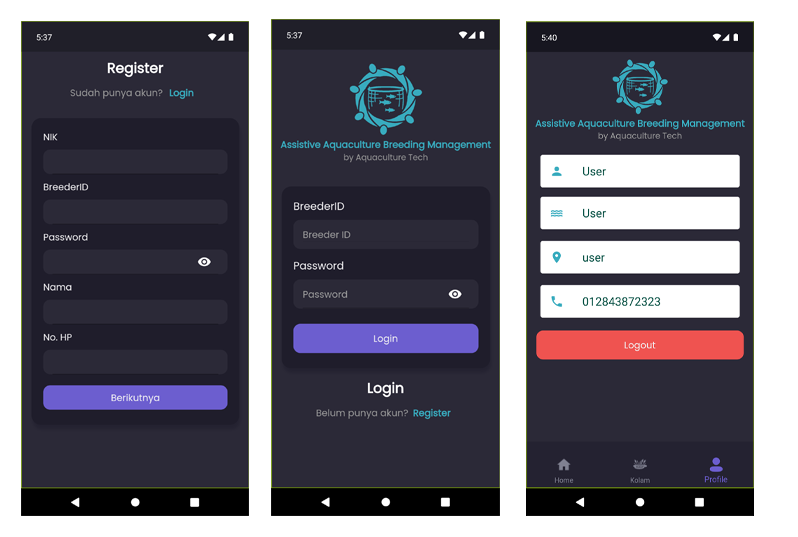
\includegraphics[keepaspectratio, width=8cm]{gambar/sssprint11}
		\caption{\textit{Output dari code pada sprint 11}}
		\label{gambar:sssprint11}
		\end{figure}

	\item{\textit{Mengitegrasikan fitur multiuser dengan webservice}}

    Hal yang dilakukan dalam mengintegrasikan fitur multiuser dengan webservice terpadat pada lampiran 12.

    \item{Analisis \textit{User Experience}} 
 
    Pada halaman register, pembudidaya harus memasukan data yang diperlukan untuk melakukan register sesuai dengan kesepakatan saat meeting. Setelah melakukan pendaftaran/register user dapat melakukan login dengan akun yang telah didaftarkan dengan menggunakan breeder ID dan password. Terdapat pula halaman profile yang berisi informasi yang terkait akun user/pembudidaya, dihalaman tersebut user dapat melakukan logout.
  

\item{Sprint 11 Review}

Sprint 11 diakhiri dengan melakukan weekly meeting pada hari selasa dengan agenda melakukan review dan testing terkait hasil sprint 11 dan melakukan planning untuk testing keseluruhan dengan rincian:
\begin{enumerate}
	\item{\textit{Review dan Testing hasil dari sprint 11}}

  Telah dilakukan review dan testing oleh penulis selaku developer dengan Scrum Master. Setelah dilakukan testing, Scrum Master menyimpulkan bahwa fitur multiuser telah berjalan dengan baik.

  \begin{longtable}{| p{8cm} | c | c | l |}
    \caption{Unit testing Halaman Awal.\label{table:unit_testing_fitur_awal}}\\
    \hline
    \multirow{2}{*}{Skenario Pengujian} & \multicolumn{2}{l|}{Kesesuaian} & \multirow{2}{*}{Kesimpulan} \\ 
    \cline{2-3}
      & \multicolumn{1}{l|}{sesuai} & tidak sesuai & \\ 
    \hline
    \hline
    \endfirsthead
    \hline
    \multirow{2}{*}{Skenario Pengujian} & \multicolumn{2}{l|}{Kesesuaian} & \multirow{2}{*}{Kesimpulan} \\ 
    \cline{2-3}
      & \multicolumn{1}{l|}{sesuai} & tidak sesuai &  \\ 
    \hline
    \hline
    \endhead
    \hline
    \endfoot
    
    
    \hline\hline
    \endlastfoot
    Saat aplikasi dibuka akan muncul splash screen yang menampilkan logo yang menandakan aplikasi sedang loading & \Checkmark &  & Diterima \\ 
    \hline
    Setelah loading selesai maka akan ditampikan halaman login & \Checkmark & & Diterima \\ 
    \hline
    \end{longtable}
    
    
    \begin{longtable}{| p{8cm} | c | c | l |}
    \caption{Unit testing Halaman Login.\label{table:unit_testing_fitur_login}}\\
    \hline
    \multirow{2}{*}{Skenario Pengujian} & \multicolumn{2}{l|}{Kesesuaian} & \multirow{2}{*}{Kesimpulan} \\ 
    \cline{2-3}
      & \multicolumn{1}{l|}{sesuai} & tidak sesuai & \\ 
    \hline
    \hline
    \endfirsthead
    \hline
    \multirow{2}{*}{Skenario Pengujian} & \multicolumn{2}{l|}{Kesesuaian} & \multirow{2}{*}{Kesimpulan} \\ 
    \cline{2-3}
      & \multicolumn{1}{l|}{sesuai} & tidak sesuai &  \\ 
    \hline
    \hline
    \endhead
    \hline
    \endfoot
    
    
    \hline\hline
    \endlastfoot
     Ketika mengisi form login dengan data yang sesuai kemudian menekan submit, maka akan masuk ke halaman dashboard & \Checkmark &  & Diterima \\ 
    \hline
     Ketika mengisi form login dengan data yang tidak sesuai kemudian menekan submit, maka akan menampilkan pesan kesalahan & \Checkmark & & Diterima \\ 
    \hline
    \end{longtable}
\end{enumerate}
\end{enumerate}

\section{Pengujian Sistem}
Pengujian sistem dilakukan menggunakan dua tipe yaitu Unit Testing dan User Acceptance Test (UAT). Pengujian dilaksanakan pada saat seluruh User Story pada Product Backlog telah diimplementasikan. Unit testing aplikasi dilakukan terhadap satu frontend developer, sedangkan pengujian User Acceptance Test dilakukan terhadap satu scrum master dan owner.

\subsection {Unit Testing}

Adapun hasil dari unit testing yang telah dilaksanakan kepada salah satu developer internal, pengujian tersebut dilakukan pada saat suatu fitur telah dinyatakan selesai yang dimana hasil unit testing tersebut telah dijelaskan pada masing masing sprint report sebelumnya. Kesimpulan dari unit testing yang telah dilakukan adalah fitur yang telah dibuat dapat berjalan dengan baik.

\subsection {User Acceptance Testing}

User Acceptance Test terhadap user dilaksanakan pada tanggal 22 April 2023 secara luring bertempat di kecamatan jasinga. Adapun hasil dari UAT yang telah dilaksanakan dapat dilihat pada tabel dibawah ini.

 \begin{longtable}[c]{@{} |p{1cm}|p{6.5cm}|p{1.1cm}|p{1.1cm}|p{1.1cm}|p{1.1cm}| @{}}
    \caption{\textit{User Acceptance Test} \label{user_testing}}\\
   
    \hline
    \multicolumn{6}{| c |}{\textbf{\textit{User Acceptance Test}}}\\
    \hline
     \multirow{2}{=}{\centering{\textbf{No}}} & \multirow{2}{=}{\centering{\textbf{\textit{Acceptance Requirements}}}} & \multicolumn{4}{| c |}{\textbf{Kesesuaian}}\\
    \cline{3-6}
      &  & \centering{\textbf{SS}} & \centering{\textbf{S}} & \centering{\textbf{TS}} & \centering{\textbf{STS}}
    \endfirsthead
   
    \hline
    \multicolumn{6}{| c |}{\textbf{\textit{User Acceptance Test}}}\\
    \hline
     \multirow{2}{=}{\centering{\textbf{No}}} & \multirow{2}{=}{\centering{\textbf{\textit{Acceptance Requirements}}}} & \multicolumn{4}{| c |}{\textbf{Kesesuaian}}\\
    \cline{3-6}
     &  & \centering{\textbf{SS}} & \centering{\textbf{S}} & \centering{\textbf{TS}} & \centering{\textbf{STS}}
    \endhead
   
    \hline
    \endfoot
   
    \hline
    \endlastfoot
   
    \hline
    1 & Fitur login sudah sesuai dengan kebutuhan pembudidaya & \Checkmark &  &  &\\
    \hline
    2 & Fitur dasboard sudah sesuai dengan kebutuhan pembudidaya & \Checkmark &  &  &\\
    \hline
    3 & Fitur registrasi, aktivasi dan deaktivasi sudah sesuai dengan kebutuhan pembudidaya &  &  & \Checkmark &\\
    \hline
    4 & Fitur pemberian dan rekapitulasi pakan sudah sesuai dengan kebutuhan pembudidaya &  & \Checkmark &  &\\
    \hline
    5 & Fitur grading berat ikan sudah sesuai dengan kebutuhan pembudidaya & \Checkmark &  &  &\\
    \hline
    6 & Fitur pencatatan kematian sudah sesuai dengan kebutuhan pembudidaya & \Checkmark &  &  &\\
    \hline
    7 & Fitur treatment kolam sudah sesuai dengan kebutuhan pembudidaya & \Checkmark &  &  &\\
    \hline
    8 & Fitur pencatatan kualitas air harian sudah sesuai dengan kebutuhan pembudidaya &  &  & \Checkmark &\\
    \hline
    9 & Fitur pencatatan kualitas air mingguan sudah sesuai dengan kebutuhan pembudidaya &  &  & \Checkmark &\\
    \hline
    10 & Fitur sortir ikan sudah sesuai dengan kebutuhan pembudidaya &  &  & \Checkmark &\\
    \hline
    \end{longtable}

Berdasarkan tabel diatas, terdapat empat fitur yang memerlukan revisi diantaranya:

\begin{enumerate}
	\item Pada fitur aktivasi kolam perlu ditambahkan input tipe aktivasi, yaitu pada saat melakukan aktivasi dapat memilih tipe aktivasinya dengan pilihan pembenihan dan pembesaran. 
	\item Pada fitur pencatatan kualitas air harian inputnya perlu diubah ke dalam bentuk desimal dikarenakan ukuran pH, Dissolved Oxygen. dan suhu dapat berupa desimal.
	\item Pada fitur pencatatan kualitas air mingguan inputnya perlu diubah ke dalam format desimal dikarenakan data yang di input dapat berupa desimal.
	\item Pada fitur sortir, terdapat perubahan flow dari fitur tersebut agar lebih sesuai dengan sortir ikan yang dilakukan oleh pembudidaya di lapangan.
\end{enumerate}

\subsection {Kesimpulan Pengujian}

Pengujian aplikasi dilaksanakan dengan dua metode yaitu unit testing dan User Acceptance Test (UAT). Berdasarkan uraian di atas, seluruh skenario pada unit testing terhadap satu internal developer berjalan dengan baik. Namun, berdasarkan hasil UAT terhadap pembudidaya terdapat beberapa masukan seperti fitur aktivasi kolam, pencatatan kualitas air, dan fitur sortir kolam.


%\subsection{\textit{Daily Scrum}}

%Pada akhir pekan di akhir setiap \textit{sprint}, akan diadakan \textit{voice call} untuk membahas perkembangan dan hambatan pada setiap \textit{sprint}.

% Baris ini digunakan untuk membantu dalam melakukan sitasi
% Karena diapit dengan comment, maka baris ini akan diabaikan
% oleh compiler LaTeX.
\begin{comment}
\bibliography{daftar-pustaka}
\end{comment}
%!TEX root = ./template-skripsi.tex
%-------------------------------------------------------------------------------
%                            	BAB IV
%               		KESIMPULAN DAN SARAN
%-------------------------------------------------------------------------------

\chapter{KESIMPULAN DAN SARAN}

\section{Kesimpulan}
Berdasarkan hasil implementasi dan pengujian fitur yang telah dirancang, maka diperoleh kesimpulan sebagai berikut:

\begin{enumerate}
	\item Terciptanya aplikasi pendukung teknologi perikanan modern versi pertama yang sudah mengintegrasikan fitur-fitur pada Product Backlog. Adapun perancangannya dilakukan dengan metode Scrum dengan tahapan penyusunan Product Backlog, Sprint Backlog, dan dikerjakan dalam sebelas Sprint.
	
	\item Berdasarkan hasil pengujian, seluruh skenario pada unit testing terhadap satu internal developer berjalan dengan baik. Namun, berdasarkan hasil UAT terhadap pembudidaya terdapat beberapa masukan seperti Pada fitur aktivasi kolam perlu ditambahkan input tipe aktivasi, apakah aktivasi tersebut atau pembesaran , pada fitur kualitas air inputnya perlu bisa dalam format desimal, dan pada fitur sortir, terdapat perubahan flow agar lebih sesuai dengan sortir ikan yang dilakukan oleh pembudidaya.
\end{enumerate}

\section{Saran}
Adapun saran untuk penelitian selanjutnya adalah:
\begin{enumerate} 
	\item Berdasarkan diskusi dengan user/product owner, harus dimulainya pengembangan sistem berikutnya yang memiliki fitur invetarisasi dan penentuan harga jual ikan agar dapat membantu pembudidaya dalam menentukan harga hasil buidayanya.
	\item Berdasarkan diskusi dengan scrum master, perlu ditambahkan feedback dari sistem seperti pop up atau sejenisnya setelah berinteraksi dengan sistem, apakah interaksi yang dilakukan dengan sistem berhasil atau tidak.
\end{enumerate}


% Baris ini digunakan untuk membantu dalam melakukan sitasi
% Karena diapit dengan comment, maka baris ini akan diabaikan
% oleh compiler LaTeX.
\begin{comment}
\bibliography{daftar-pustaka}
\end{comment}

%-----------------------------------------------------------------
%Disini akhir masukan Bab
%-----------------------------------------------------------------


%-----------------------------------------------------------------
% Disini awal masukan untuk Daftar Pustaka
% - Daftar pustaka diambil dari file .bib yang ada pada folder ini
%   juga.
% - Untuk memudahkan dalam memanajemen dan menggenerate file .bib
%   gunakan reference manager seperti Mendeley, Zotero, EndNote,
%   dll.
%-----------------------------------------------------------------
\bibliography{daftar-pustaka}
\bibliographystyle{myapalike}
\addcontentsline{toc}{chapter}{DAFTAR PUSTAKA}
\addcontentsline{toc}{chapter}{LAMPIRAN}
\setcounter{section}{0}
\chapter*{\centering{\large{LAMPIRAN}}}

\section{Lampiran 1 Transkrip Percakapan}
\begin{flushleft}
Hari: Selasa
\linebreak
Tanggal: 23 Agustus 2022
\linebreak
P: Penulis
\linebreak
K: Klien (UD Jfarm)
\linebreak
\linebreak
P: Sistem apa yang akan di buat?
\linebreak
K: Kita akan membuat frontend untuk aplikasi pendukung teknologi perikanan modern
\linebreak
P: Apa saja requirement yang diperlukan dalam aplikasi tersebut?
\linebreak
K: Requirementnya adalah penerapan fitur yang sudah ada dalam backend penelitian dari Andri Rahmanto yang berbentuk REST API.
\linebreak
P: Apa saja fitur yang ada dalam backend yang telah dibuat dalam penelitian Andri Rahmanto?
\linebreak
K: Fiturnya adalah pencatatan pemberian pakan, registrasi kolam, aktifasi-deaktifasi kolam, pencatatan kulaitas air harian dan mingguan, pencatatan data kematian harian, pencatatan treatment kolam, grading berat ikan, dan sortir ikan.
\linebreak
\end{flushleft}



\clearpage
\section{Lampiran 2 code untuk sprint 1 report}
\lstset{frame=tb,
	  language=c++,
	  aboveskip=5mm,
	  belowskip=5mm,
	  showstringspaces=false,
	  columns=flexible,
	  basicstyle={\scriptsize\ttfamily},
	  numbers=none,
	  breaklines=true,
	  breakatwhitespace=true,
	  tabsize=3}

	\begin{lstlisting}
	    Widget title() {
	      return Container(
	        margin: EdgeInsets.only(
	          top: defaultMargin,
	          left: defaultMargin,
	          right: defaultMargin,
	        ),
	        child: Text(
	          'Home',
	          style: primaryTextStyle.copyWith(
	            fontSize: 24,
	            fontWeight: semiBold,
	          ),
	        ),
	      );
	    }
	
	    Widget statistic() {
	      return Container(
	          margin: EdgeInsets.only(
	            top: defaultMargin,
	            left: defaultMargin,
	          ),
	          child: Column(
	            crossAxisAlignment: CrossAxisAlignment.center,
	            mainAxisAlignment: MainAxisAlignment.center,
	            children: [
	              Row(
	                mainAxisAlignment: MainAxisAlignment.spaceBetween,
	                crossAxisAlignment: CrossAxisAlignment.center,
	                children: [
	                  Expanded(
	                      flex: 1,
	                      child: StatisticCard(
	                        title: 'Kolam',
	                        value: controller.statistic.value.total_pond,
	                      )),
	                  Expanded(
	                      flex: 1,
	                      child: StatisticCard(
	                        title: 'Kolam Aktif',
	                        value: controller.statistic.value.active_pond,
	                      )),
	                ],
	              ),
	              SizedBox(
	                height: 16,
	              ),
	              Row(
	                mainAxisAlignment: MainAxisAlignment.spaceBetween,
	                crossAxisAlignment: CrossAxisAlignment.center,
	                children: [
	                  Expanded(
	                      flex: 1,
	                      child: StatisticCard(
	                        title: 'Ikan Hidup',
	                        value: controller.statistic.value.fish_live,
	                        unit: 'Ekor',
	                      )),
	                  Expanded(
	                      flex: 1,
	                      child: StatisticCard(
	                        title: 'Ikan Mati',
	                        value: controller.statistic.value.fish_death,
	                        unit: 'Ekor',
	                      )),
	                ],
	              ),
	              SizedBox(
	                height: 16,
	              ),
	              Row(
	                mainAxisAlignment: MainAxisAlignment.spaceBetween,
	                crossAxisAlignment: CrossAxisAlignment.center,
	                children: [
	                  Expanded(
	                      flex: 1,
	                      child: StatisticCard(
	                        title: 'Panen 2022',
	                        value: controller.statistic.value.fish_harvested,
	                        unit: 'Kg',
	                      )),
	                  Expanded(
	                      flex: 1,
	                      child: StatisticCard(
	                        title: 'Total Pakan',
	                        value: controller.statistic.value.total_feed_dose,
	                        unit: 'Kg',
	                      )),
	                ],
	              ),
	            ],
	          ));
	    }
	\end{lstlisting}
	

\textit{Lampiran 3 code widget untuk section statistik ikan}
\begin{lstlisting}
	Widget fishTitle() {
	  return Container(
		margin: EdgeInsets.only(
		  top: defaultSpace,
		  left: defaultMargin,
		  right: defaultMargin,
		),
		child: Column(
		  crossAxisAlignment: CrossAxisAlignment.start,
		  children: [
			Text(
			  'Total Berat Ikan',
			  style: primaryTextStyle.copyWith(
				fontSize: 24,
				fontWeight: semiBold,
			  ),
			),
		  ],
		),
	  );
	}

	Widget fish() {
	  return Container(
		margin: EdgeInsets.only(top: 14),
		child: SingleChildScrollView(
		  scrollDirection: Axis.horizontal,
		  child: Row(
			children: [
			  SizedBox(
				width: defaultMargin,
			  ),
			  Row(children: [
				FishCard(
				  title: "Lele",
				  value: controller.statistic.value.fishes_weight_lele!,
				  image: "assets/lele.png",
				),
				FishCard(
				  title: "Nila Merah",
				  value: controller.statistic.value.fishes_weight_nilamerah!,
				  image: "assets/nilamerah.png",
				),
				FishCard(
				  title: "Nila Hitam",
				  value: controller.statistic.value.fishes_weight_nilahitam!,
				  image: "assets/nilahitam.png",
				),
				FishCard(
				  title: "Mas",
				  value: controller.statistic.value.fishes_weight_mas!,
				  image: "assets/mas.png",
				),
			  ]),
			],
		  ),
		),
	  );
	}
\end{lstlisting}


\textit{code widget untuk section statistik kondisi air}
\begin{lstlisting}
	Widget waterTitle() {
	  return Container(
		margin: EdgeInsets.only(
		  top: defaultSpace,
		  left: defaultMargin,
		  right: defaultMargin,
		),
		child: Column(
		  crossAxisAlignment: CrossAxisAlignment.start,
		  children: [
			Text(
			  'Kualitas Air',
			  style: primaryTextStyle.copyWith(
				fontSize: 24,
				fontWeight: semiBold,
			  ),
			),
		  ],
		),
	  );
	}

	Widget water() {
	  return Container(
		margin: EdgeInsets.only(top: 14),
		child: SingleChildScrollView(
		  scrollDirection: Axis.horizontal,
		  child: Row(
			children: [
			  SizedBox(
				width: defaultMargin,
			  ),
			  Row(children: [
				WaterCard(
				  title: "pH",
				  normal: controller.statistic.value.ph_normal,
				  abnormal: controller.statistic.value.ph_abnormal,
				),
				WaterCard(
				  title: "DO",
				  normal: controller.statistic.value.do_normal,
				  abnormal: controller.statistic.value.do_abnormal,
				),
				WaterCard(
				  title: "Flok",
				  normal: controller.statistic.value.floc_normal,
				  abnormal: controller.statistic.value.floc_abnormal,
				),
			  ]),
			],
		  ),
		),
	  );
	}
\end{lstlisting}



\textit{code widget untuk bagian bottom navigation bar}
\begin{lstlisting}
	bottomNavigationBar: BottomNavigationBar(
            type: BottomNavigationBarType.fixed,
            backgroundColor: backgroundColor3,
            onTap: controller.changeTabIndex,
            currentIndex: controller.tabIndex,
            items: [
              BottomNavigationBarItem(
                icon: Container(
                  margin: EdgeInsets.only(
                    top: 20,
                    bottom: 5,
                  ),
                  child: Image.asset(
                    'assets/home_secondary.png',
                    width: 25,
                    color: controller.tabIndex == 0
                        ? primaryColor
                        : Color(0xff808191),
                  ),
                ),
                label: '',
              ),
              BottomNavigationBarItem(
                icon: Container(
                  margin: EdgeInsets.only(
                    top: 20,
                    bottom: 5,
                  ),
                  child: Image.asset(
                    'assets/pond_secondary.png',
                    width: 25,
                    color: controller.tabIndex == 1
                        ? primaryColor
                        : Color(0xff808191),
                  ),
                ),
                label: '',
              ),
            ],
          ),
	\end{lstlisting}

	


\textit{Mengintegrasikan dengan webservice}

	\textit{Model Class untuk Halaman Dashboard}
	\begin{lstlisting}
	class StatisticModel {
  	int? total_pond;
  	int? active_pond;
  	int? fish_live;
  	int? fish_death;
  	int? fish_harvested;
  	int? total_feed_dose;
  	num? fishes_weight_lele;
  	num? fishes_weight_nilamerah;
  	num? fishes_weight_nilahitam;
  	num? fishes_weight_mas;
  	num? fishes_weight_patin;
  	int? ph_normal;
  	int? ph_abnormal;
  	int? do_normal;
  	int? do_abnormal;
  	int? floc_normal;
	  int? floc_abnormal;

	  StatisticModel(
	      {this.total_pond,
	      this.active_pond,
	      this.fish_live,
	      this.fish_death,
	      this.fish_harvested,
	      this.total_feed_dose,
	      this.fishes_weight_lele,
	      this.fishes_weight_nilamerah,
	      this.fishes_weight_nilahitam,
	      this.fishes_weight_mas,
	      this.fishes_weight_patin,
	      this.ph_normal,
	      this.ph_abnormal,
	      this.do_normal,
	      this.do_abnormal,
	      this.floc_normal,
	      this.floc_abnormal});

	  StatisticModel.fromJson(Map<String, dynamic> json) {
	    total_pond = json['total_pond'];
	    active_pond = json['active_pond'];
	    fish_live = json['fish_live'];
	    fish_death = json['fish_death'];
	    fish_harvested = json['fish_harvested'];
	    total_feed_dose = json['total_feed_dose'];
	    fishes_weight_nilahitam = json['fishes_weight'][0]["amount"];
	    fishes_weight_nilamerah = json['fishes_weight'][1]["amount"];
	    fishes_weight_lele = json['fishes_weight'][2]["amount"];
	    fishes_weight_patin = json['fishes_weight'][3]["amount"];
	    fishes_weight_mas = json['fishes_weight'][4]["amount"];
	    ph_normal = json['water_quality']['ph']['normal'];
	    ph_abnormal = json['water_quality']['ph']['abnormal'];
	    do_normal = json['water_quality']['do']['normal'];
	    do_abnormal = json['water_quality']['do']['abnormal'];
	    floc_normal = json['water_quality']['floc']['normal'];
	    floc_abnormal = json['water_quality']['floc']['abnormal'];
	  }
	}
	\end{lstlisting}

	\textit{ Networt Request untuk Halaman Dashboard }
	\begin{lstlisting}
	import 'dart:convert';
	import 'package:fish/models/statistic_model.dart';
	import 'package:fish/service/url_api.dart';
	import 'package:http/http.dart' as http;
	
	class StatisticService {
	  Future<StatisticModel> getStatistic() async {
	    var url = Uri.parse('http://jft.web.id/fishapi/api/statistic');
	    var headers = {'Content-Type': 'application/json'};
	
	    var response = await http.get(url, headers: headers);
	
	    print(response.body);
	
	    if (response.statusCode == 200) {
	      var data = jsonDecode(response.body);
	      StatisticModel statistic = StatisticModel.fromJson(data);
	
	      return statistic;
	    } else {
	      throw Exception('Gagal Get Products!');
	    }
	  }
	}
	
	\end{lstlisting}

	\textit{ Mengolah data yang telah direquest pada Controller }
	\begin{lstlisting}
	class HomeController extends GetxController {
	  var isLoading = false.obs;
	
	  final statistic = StatisticModel().obs;
	
	  @override
	  void onInit() async {
	    await getStatisticData();
	    super.onInit();
	  }
	
	  Future<void> getStatisticData() async {
	    isLoading.value = true;
	    StatisticModel statisticData = await StatisticService().getStatistic();
	    statistic.value = statisticData;
	    Timer(const Duration(seconds: 1), () {
	      isLoading.value = false;
	    });
	  }
	}

	\end{lstlisting}

	\textit{Menampilkan data pada Halaman Dashboard}
	\begin{lstlisting}
	Widget water() {
	      return Container(
	        margin: EdgeInsets.only(top: 14),
	        child: SingleChildScrollView(
	          scrollDirection: Axis.horizontal,
	          child: Row(
	            children: [
	              SizedBox(
	                width: defaultMargin,
	              ),
	              Row(children: [
	                WaterCard(
	                  title: "pH",
	                  normal: controller.statistic.value.ph_normal,
	                  abnormal: controller.statistic.value.ph_abnormal,
	                ),
	                WaterCard(
	                  title: "DO",
	                  normal: controller.statistic.value.do_normal,
	                  abnormal: controller.statistic.value.do_abnormal,
	                ),
	                WaterCard(
	                  title: "Flok",
	                  normal: controller.statistic.value.floc_normal,
	                  abnormal: controller.statistic.value.floc_abnormal,
	                ),
	              ]),
	            ],
	          ),
	        ),
	      );
	    }
	\end{lstlisting}

\clearpage
\section{Lampiran 3 Sprint 2 report}
\begin{lstlisting}
	import 'package:fish/models/pond_model.dart';
	import 'package:fish/pages/component/pond_card.dart';
	
	import 'package:fish/pages/pond/add_pond_page.dart';
	import 'package:fish/pages/pond/pond_controller.dart';
	import 'package:flutter/material.dart';
	import 'package:fish/theme.dart';
	import 'package:get/get.dart';
	
	class PondPage extends StatefulWidget {
	  PondPage({Key? key}) : super(key: key);
	  @override
	  State<PondPage> createState() => _PondPageState();
	}
	
	class _PondPageState extends State<PondPage> {
	  final PondController controller = Get.put(PondController());
	  int? _value = null;
	  final chip = ["Aktif", "Panen", "Tidak Aktif"];
	  @override
	  void initState() {
		super.initState();
	
		controller.getPondsData(context);
	  }
	
	  @override
	  Widget build(BuildContext context) {
		Widget title() {
		  return Container(
			margin: EdgeInsets.only(
			  top: defaultMargin,
			  left: defaultMargin,
			  right: defaultMargin,
			),
			child: Text(
			  'Kolam',
			  style: primaryTextStyle.copyWith(
				fontSize: 24,
				fontWeight: semiBold,
			  ),
			),
		  );
		}
	
		Widget filter() {
		  return Container(
			margin: EdgeInsets.only(
			  top: defaultMargin,
			  left: defaultMargin,
			  right: defaultMargin,
			),
			child: Wrap(
			  spacing: 8.0,
			  children: List<Widget>.generate(
				3,
				(int index) {
				  return ChoiceChip(
					label: Text(
					  chip[index],
					  style: TextStyle(color: Colors.white),
					),
					shape: StadiumBorder(side: BorderSide(color: Colors.white)),
					selected: _value == index,
					backgroundColor: backgroundColor1,
					selectedColor: primaryColor,
					onSelected: (bool selected) {
					  setState(() {
						_value = selected ? index : null;
						if (_value == null) {
						  controller.getPondsData(context);
						  // return null;
						} else {
						  controller.getPondsFiltered(chip[index]);
						}
					  });
					},
				  );
				},
			  ).toList(),
			),
		  );
		}
	
		Widget pondList() {
		  return Container(
			margin: EdgeInsets.only(top: 14),
			child: SingleChildScrollView(
			  child: ListView.builder(
				shrinkWrap: true,
				primary: false,
				itemBuilder: ((context, index) {
				  return PondCard(pond: controller.ponds[index]
					  // indicatorWater: controller.indicatorWater[index]);
					  );
				}),
				itemCount: controller.ponds.length,
			  ),
			),
		  );
		}
	
		Widget emptyListPond() {
		  return Container(
			  width: double.infinity,
			  margin: EdgeInsets.only(right: defaultMargin, left: defaultMargin),
			  child: Center(
				child: Column(children: [
				  SizedBox(height: 35),
				  Image(
					image: AssetImage("assets/unavailable_icon.png"),
					width: 100,
					height: 100,
					fit: BoxFit.fitWidth,
				  ),
				  SizedBox(height: 20),
				  Text(
					"Anda belum pernah melakukan registrasi kolam",
					style: primaryTextStyle.copyWith(
					  fontSize: 14,
					  fontWeight: bold,
					),
					textAlign: TextAlign.center,
					overflow: TextOverflow.ellipsis,
					maxLines: 2,
				  ),
				  SizedBox(height: 10),
				  Text(
					"Silahkan registrasi kolam",
					style: secondaryTextStyle.copyWith(
					  fontSize: 13,
					  fontWeight: bold,
					),
					textAlign: TextAlign.center,
					overflow: TextOverflow.ellipsis,
					maxLines: 2,
				  ),
				]),
			  ));
		}
	
		return Obx(() {
		  if (controller.isLoading.value == false) {
			return Scaffold(
			  backgroundColor: backgroundColor1,
			  floatingActionButton: FloatingActionButton(
				onPressed: () {
				  Get.to(() => AddPondPage());
				},
				backgroundColor: primaryColor,
				child: const Icon(Icons.add),
			  ),
			  body: ListView(
				children: [
				  title(),
				  filter(),
				  controller.ponds.isEmpty ? emptyListPond() : pondList(),
				  SizedBox(
					height: 10,
				  )
				],
			  ),
			);
		  } else {
			return Center(
			  child: CircularProgressIndicator(
				color: secondaryColor,
			  ),
			);
		  }
		});
	  }
	}
		\end{lstlisting}


\textit{Code widget untuk registrasi kolam}
\begin{lstlisting}
	import 'package:fish/pages/pond/pond_controller.dart';
	import 'package:flutter/material.dart';
	import 'package:fish/theme.dart';
	import 'package:flutter/services.dart';
	import 'package:get/get.dart';
	
	class AddPondPage extends StatefulWidget {
	  const AddPondPage({Key? key}) : super(key: key);
	
	  @override
	  State<AddPondPage> createState() => _AddPondPageState();
	}
	
	class _AddPondPageState extends State<AddPondPage> {
	  final PondController controller = Get.put(PondController());
	
	  @override
	  void dispose() {
		controller.aliasController.clear();
		controller.diameterController.clear();
		controller.heightController.clear();
		controller.locationController.clear();
		controller.lengthController.clear();
		controller.widthController.clear();
		super.dispose();
	  }
	
	  @override
	  Widget build(BuildContext context) {
	  Widget aliasInput() {...}
	  Widget locationInput() {...}
	  Widget materialInput() {...}
	  Widget shapelInput() {...}
	  Widget heightInput() {...}
	  Widget lengthInput() {...}
	  Widget widthInput() {...}
	  Widget diameterInput() {...}
	  Widget registerButton() {...}
	  Widget persegiInput() {...}
	   Widget bundarInput() {...}
	
		return Obx(() {
		  if (controller.isLoading.value == false) {
			return Scaffold(
			  appBar: AppBar(
				backgroundColor: backgroundColor2,
				title: const Text("Registrasi Kolam"),
			  ),
			  backgroundColor: backgroundColor1,
			  body: ListView(
				children: [
				  aliasInput(),
				  locationInput(),
				  materialInput(),
				  shapelInput(),
				  controller.shapeController.selected.value == 'persegi'
					  ? persegiInput()
					  : bundarInput(),
				  heightInput(),
				  registerButton(),
				  SizedBox(
					height: 8,
				  )
				],
			  ),
			);
		  } else {
			return Center(
			  child: CircularProgressIndicator(
				color: secondaryColor,
			  ),
			);
		  }
		});
	  }
	}
	
\end{lstlisting}



\textit{Code widget untuk halaman detail kolam}

\begin{lstlisting}
	import 'dart:developer';

import 'package:fish/models/pond_model.dart';
import 'package:fish/pages/component/activation_card.dart';
import 'package:fish/pages/pond/activation_breed_controller.dart';
import 'package:fish/pages/pond/activation_breed_page.dart';
import 'package:fish/pages/pond/pond_controller.dart';
import 'package:fish/pages/pond/add_pond_page.dart';
import 'package:fish/pages/pond/deactivation_breed_page.dart';
import 'package:fish/pages/pond/detail_pond_controller.dart';
import 'package:flutter/material.dart';
import 'package:fish/theme.dart';
import 'package:get/get.dart';

import '../fish_transfer/fish_transfer_entry_page.dart';

class DetailPondPage extends StatefulWidget {
const DetailPondPage({Key? key}) : super(key: key);

@override
State<DetailPondPage> createState() => _DetailPondPageState();
}

class _DetailPondPageState extends State<DetailPondPage> {
var detailController = Get.put(DetailPondController(), permanent: false);
@override
void initState() {
 super.initState();

 detailController.getPondActivation(context);
}

@override
void activate() {
 print('ini aktif');
 super.activate();
}

@override
void deactivate() {
 print('ini deaktif');
 super.deactivate();
}

@override
Widget build(BuildContext context) {
 Widget pondStatus() {...}

 Widget activationButton() {...}

 Widget deactivationButton() {...}

 Widget detail() {...}

 Widget activationTitle() {...}

 Widget listActivation() {...}

 Widget emptyListActivation() {...}

 return Scaffold(
   backgroundColor: backgroundColor1,
   body: Obx(
	 () => detailController.isLoading.value
		 ? Center(
			 child: CircularProgressIndicator(
			   color: secondaryColor,
			 ),
		   )
		 : ListView(
			 children: [
			   pondStatus(),
			   detailController.isPondActive.value == false
				   ? activationButton()
				   : deactivationButton(),
			   detail(),
			   activationTitle(),
			   detailController.activations.isEmpty
				   ? emptyListActivation()
				   : listActivation(),
			   SizedBox(
				 height: 10,
			   )
			 ],
		   ),
   ),
 );
}
}
 \end{lstlisting}


 \textit{Code halaman aktivasi kolam}

 \begin{lstlisting}
	import 'dart:developer';

import 'package:fish/pages/pond/activation_breed_controller.dart';
import 'package:fish/pages/pond/detail_pond_controller.dart';
import 'package:fish/pages/pond/detail_pond_page.dart';
import 'package:fish/service/pond_service.dart';
import 'package:fish/service/activation_service.dart';
import 'package:flutter/material.dart';
import 'package:fish/theme.dart';
import 'package:flutter/services.dart';
import 'package:get/get.dart';

import '../component/detail_pond_tabview.dart';

class ActivationBreedPage extends StatelessWidget {
  ActivationBreedPage({Key? key}) : super(key: key);

  final ActivationBreedController controller =
      Get.put(ActivationBreedController());

  final DetailPondController detailPondController =
      Get.put(DetailPondController());

  @override
  Widget build(BuildContext context) {
    Widget checkBoxFish() {...}

    Widget waterHeightInput() {...}

    Widget leleInput() {...}

    Widget nilaMerahInput() {...}

    Widget nilaHitamInput() {...}
  
    Widget patinInput() {...}

    Widget masInput() {...}

    Widget breedOptionInput() {...}

    Widget pembesaranInput() {...}

    Widget benihInput() {...}

    Widget activationButton() {...}

    return Obx(() {
      if (controller.isActivationProgress.value == false) {
        return Scaffold(
          appBar: AppBar(
            backgroundColor: backgroundColor2,
            title: const Text("Aktivasi Kolam"),
          ),
          backgroundColor: backgroundColor1,
          body: ListView(
            children: [
              breedOptionInput(),
              controller.breedOptionController.selected.value == "Benih"
                  ? benihInput()
                  : pembesaranInput(),
              checkBoxFish(),
              controller.isNilaHitam == true ? nilaHitamInput() : Container(),
              controller.isNilaMerah == true ? nilaMerahInput() : Container(),
              controller.isLele == true ? leleInput() : Container(),
              controller.isPatin == true ? patinInput() : Container(),
              controller.isMas == true ? masInput() : Container(),
              waterHeightInput(),
              activationButton(),
              SizedBox(
                height: 8,
              )
            ],
          ),
        );
      } else {
        return Center(
          child: CircularProgressIndicator(
            color: secondaryColor,
          ),
        );
      }
    });
  }
}

	\end{lstlisting}

	\clearpage
	\section{Lampiran 4 Code Sprint 3 report}
	\textit{Code untuk model class kolam}
	
	\begin{lstlisting}
	import 'package:flutter/material.dart';
import 'package:intl/intl.dart';

enum PondStatus {
  active,
  nonActive,
  close,
}

class string {}

class Pond {
  String? id;
  int? idInt;
  String? alias;
  String? location;
  String? shape;
  String? material;
  num? length;
  num? width;
  num? diameter;
  num? height;
  num? area;
  num? volume;
  String? buildAt;
  String? imageLink;
  bool? isActive;
  num? fishAlive;
  String? lastActivationDate;
  String? rangeFromLastActivation;
  PondStatus pondStatus;
  String? pondStatusStr;
  String? pondPhDesc;
  num? pondPh;
  String? pondDoDesc;
  num? pondDo;
  num? pondTemp;
  String? status;

  Pond({
    required this.id,
    required this.idInt,
    required this.alias,
    required this.location,
    required this.shape,
    required this.material,
    required this.isActive,
    required this.pondStatus,
    this.length,
    this.width,
    this.diameter,
    this.height,
    this.area,
    this.volume,
    this.buildAt,
    this.imageLink,
    this.fishAlive,
    this.lastActivationDate,
    this.rangeFromLastActivation,
    this.pondStatusStr,
    this.pondPh,
    this.pondPhDesc,
    this.pondDo,
    this.pondDoDesc,
    this.pondTemp,
    this.status,
  });

  factory Pond.fromJson(Map<String, dynamic> json) {
    return Pond(
        id: json['_id'],
        idInt: json['id_int'],
        alias: json['alias'],
        location: json['location'],
        shape: json['shape'],
        material: json['material'],
        length: json['length'],
        width: json['width'],
        diameter: json['diameter'],
        height: json['height'],
        area: json['area'],
        volume: json['volume'],
        buildAt: json['build_at'],
        imageLink: json['image_link'],
        isActive: json['isActive'],
        fishAlive: json['fish_alive'] ?? 0,
        lastActivationDate: json['activation_date'] ?? "-",
        rangeFromLastActivation: json['isActive'] == false
            ? "-"
            : (DateTime.now()
                    .difference(stringToDate(json['activation_date']))
                    .inDays)
                .toString(),
        pondStatus: PondStatusConverter.toEnum(json["status"]),
        pondStatusStr: json["status"],
        pondPh: json["pondPh"],
        pondPhDesc: json["pondPhDesc"],
        pondDo: json["pondDo"],
        pondDoDesc: json["pondDoDesc"],
        pondTemp: json["pondTemp"],
        status: json["status"]);
  }

  static DateTime stringToDate(String dateString) {
    DateTime parseDate = DateFormat("dd-MM-yyyy").parse(dateString);
    return parseDate;
  }

  Color getColor() {
    PondStatus pondStatus = this.pondStatus;
    switch (pondStatus) {
      case PondStatus.active:
        return Colors.green;
      case PondStatus.nonActive:
        return Colors.red.shade300;
      case PondStatus.close:
        return Colors.amber;
      default:
        return Colors.red.shade300;
    }
  }

  String getFishAlive() {
    if (isActive == false) {
      return '-';
    } else {
      return fishAlive.toString();
    }
  }

  String getLastActivationDate() {
    if (isActive == false) {
      return '-';
    } else {
      return lastActivationDate!;
    }
  }

  String getGmtToNormalDate() {
    String stringDate = buildAt!;
    DateTime dateTime = DateFormat("yyyy-MM-dd hh:mm:ss").parse(stringDate);
    String newStringDate = DateFormat("dd-MM-yyyy").format(dateTime);
    return newStringDate;
  }
}

extension PondStatusConverter on PondStatus {
  static PondStatus toEnum(String? status) {
    switch (status) {
      case 'Aktif':
        return PondStatus.active;
      case 'Tidak Aktif':
        return PondStatus.nonActive;
      case 'Panen':
        return PondStatus.close;
      default:
        return PondStatus.nonActive;
    }
  }
}
	\end{lstlisting}

	\textit{Code untuk API service halaman terkait kolam kolam}
	
	\begin{lstlisting}
import 'dart:convert';
import 'dart:math';
import 'package:fish/models/pond_model.dart';
import 'package:fish/service/url_api.dart';
import 'package:flutter/material.dart';
import 'package:http/http.dart' as http;
import 'package:shared_preferences/shared_preferences.dart';

import '../theme.dart';

class PondService {
  Future<List<Pond>> getPonds() async {
    WidgetsFlutterBinding.ensureInitialized();
    SharedPreferences prefs = await SharedPreferences.getInstance();
    String token = prefs.getString('token').toString();
    var url = Uri.parse(Urls.ponds);
    var headers = {
      'Content-Type': 'application/json',
      'Authorization': 'Bearer $token'
    };

    var response = await http.get(url, headers: headers);

    print(response.body);

    if (response.statusCode == 200) {
      var data = jsonDecode(response.body);
      List<Pond> ponds = [];

      for (var item in data) {
        ponds.add(Pond.fromJson(item));
      }

      print(ponds);

      return ponds;
    } else {
      throw Exception(e);
    }
  }

  Future<void> getPondDetail({required String pondId}) async {
    var url = Uri.parse(Urls.pond(pondId));
    var headers = {'Content-Type': 'application/json'};

    var response = await http.get(url, headers: headers);

    print(response.body);

    if (response.statusCode == 200) {
      var data = jsonDecode(response.body);
      // Pond pond = Pond.fromJson(data);
      // print(pond);

      // return pond;
    } else {
      throw Exception('Gagal Get Detial Pond!');
    }
  }

  Future<bool> pondRegister(
      {required String? alias,
      required String? location,
      required String? shape,
      required String? material,
      required String? length,
      required String? width,
      required String? diameter,
      required String? height,
      required String? status,
      required Function doInPost,
      required BuildContext context}) async {
    if (diameter!.isNotEmpty) {
      if (diameter.contains(",")) {
        diameter = diameter.replaceAll(',', '.');
      }
    }
    if (length!.isNotEmpty) {
      if (length.contains(",")) {
        length = length.replaceAll(',', '.');
      }
    }
    if (width!.isNotEmpty) {
      if (width.contains(",")) {
        width = width.replaceAll(',', '.');
      }
    }
    if (height!.isNotEmpty) {
      if (height.contains(",")) {
        height = height.replaceAll(',', '.');
      }
    }
    WidgetsFlutterBinding.ensureInitialized();
    SharedPreferences prefs = await SharedPreferences.getInstance();
    String token = prefs.getString('token').toString();
    final response = await http.post(
      Uri.parse(Urls.ponds),
      headers: {
        "Content-Type": "application/x-www-form-urlencoded",
        'Authorization': 'Bearer $token'
      },
      encoding: Encoding.getByName('utf-8'),
      body: {
        "alias": alias,
        "location": location,
        "shape": shape,
        "material": material,
        "status": status,
        "length": length,
        "width": width,
        "diameter": diameter,
        "height": height,
      },
    );

    if (response.statusCode == 200) {
      doInPost();
      Navigator.pop(context);
      return true;
    } else {
      var res = jsonDecode(response.body);

      showDialog<String>(
          context: context,
          builder: (BuildContext context) => AlertDialog(
                title: const Text('Input Error',
                    style: TextStyle(color: Colors.red)),
                content: Text(
                  '${res["message"]}',
                  style: TextStyle(color: Colors.white),
                ),
                backgroundColor: backgroundColor1,
                shape: RoundedRectangleBorder(
                    borderRadius: BorderRadius.all(Radius.circular(16.0))),
                actions: <Widget>[
                  TextButton(
                    onPressed: () => Navigator.pop(context, 'OK'),
                    child: const Text('OK'),
                  ),
                ],
              ));
      return false;
    }
  }
}
	\end{lstlisting}
	
	\textit{Code widget untuk halaman pemberian pakan}
	\begin{lstlisting}
import 'package:fish/models/feed_chart_model.dart';
import 'package:fish/pages/component/feed_month_card.dart';
import 'package:fish/pages/feeding/feed_controller.dart';
import 'package:fish/pages/pond/detail_pond_controller.dart';
import 'package:fish/pages/pond/pond_controller.dart';
import 'package:flutter/material.dart';
import 'package:fish/pages/feeding/feed_entry_page.dart';
import 'package:fish/theme.dart';
import 'package:get/get.dart';
import 'package:syncfusion_flutter_charts/charts.dart';

class DetailFeedPage extends StatelessWidget {
  const DetailFeedPage({Key? key}) : super(key: key);

  @override
  Widget build(BuildContext context) {
    final FeedController controller = Get.put(FeedController());
    final PondController pondController = Get.find();
    final DetailPondController detailPondController = Get.find();

    Widget chartFeed() {...}

    Widget emptyListPond() {...}

    Widget feedDataRecap() {...}

    Widget entryPakanButton() {...}

    Widget detail() {...}

    Widget recapTitle() {...}

    Widget listMonthFeed() {...}

    return Obx(() {
      if (controller.isLoading.value == false) {
        return Scaffold(
          appBar: AppBar(
            backgroundColor: backgroundColor2,
            title: const Text("Detail Pakan Permusim"),
          ),
          backgroundColor: backgroundColor1,
          body: ListView(
            children: [
              chartFeed(),
              feedDataRecap(),
              // detail(),
              entryPakanButton(),
              recapTitle(),
              // chartRecap(),
              controller.list_feedHistoryMonthly.isEmpty
                  ? emptyListPond()
                  : listMonthFeed(),
              SizedBox(
                height: 10,
              )
            ],
          ),
        );
      } else {
        return Center(
          child: CircularProgressIndicator(
            color: secondaryColor,
          ),
        );
      }
    });
  }
}

	\end{lstlisting}

	\textit{Code untuk halaman entry pakan}
	\begin{lstlisting}
import 'package:fish/pages/feeding/feed_entry_controller.dart';
import 'package:flutter/material.dart';
import 'package:fish/theme.dart';
import 'package:flutter/services.dart';
import 'package:get/get.dart';

import 'feed_controller.dart';

class FeedEntryPage extends StatelessWidget {
  const FeedEntryPage({Key? key}) : super(key: key);

  @override
  Widget build(BuildContext context) {
    final FeedEntryController controller = Get.put(FeedEntryController());
    final FeedController feedcontroller = Get.put(FeedController());

    Widget feedTypeInput() {
      return Container(
        margin: EdgeInsets.only(
            top: defaultSpace, right: defaultMargin, left: defaultMargin),
        child: Column(
          crossAxisAlignment: CrossAxisAlignment.start,
          children: [
            Text(
              'Pilih Pakan',
              style: primaryTextStyle.copyWith(
                fontSize: 16,
                fontWeight: medium,
              ),
            ),
            SizedBox(
              height: 12,
            ),
            Container(
              height: 50,
              padding: EdgeInsets.symmetric(
                horizontal: 16,
              ),
              decoration: BoxDecoration(
                color: backgroundColor2,
                borderRadius: BorderRadius.circular(12),
              ),
              child: Center(
                child: Obx(() => DropdownButtonFormField<String>(
                      onChanged: (newValue) => controller.feedTypeFormController
                          .setSelected(newValue!),
                      value: controller.feedTypeFormController.selected.value,
                      items: controller.feedTypeFormController.listFeedType
                          .map((feedtype) {
                        return DropdownMenuItem<String>(
                          value: feedtype.type,
                          child: Text(
                            feedtype.type.toString(),
                            style: primaryTextStyle,
                          ),
                        );
                      }).toList(),
                      dropdownColor: backgroundColor5,
                      decoration: InputDecoration(border: InputBorder.none),
                    )),
              ),
            ),
          ],
        ),
      );
    }

    Widget feedSatuanInput() {
      return Container(
        margin: EdgeInsets.only(
            top: defaultSpace, right: defaultMargin, left: defaultMargin),
        child: Column(
          crossAxisAlignment: CrossAxisAlignment.start,
          children: [
            Text(
              'Pilih Satuan',
              style: primaryTextStyle.copyWith(
                fontSize: 16,
                fontWeight: medium,
              ),
            ),
            SizedBox(
              height: 12,
            ),
            Container(
              height: 50,
              padding: EdgeInsets.symmetric(
                horizontal: 16,
              ),
              decoration: BoxDecoration(
                color: backgroundColor2,
                borderRadius: BorderRadius.circular(12),
              ),
              child: Center(
                child: Obx(() => DropdownButtonFormField<String>(
                      onChanged: (newValue) => controller.feedSatuanController
                          .setSelected(newValue!),
                      value: controller.feedSatuanController.selected.value,
                      items: controller.feedSatuanController.listSatuan
                          .map((feedtype) {
                        return DropdownMenuItem<String>(
                          value: feedtype,
                          child: Text(
                            feedtype.toString(),
                            style: primaryTextStyle,
                          ),
                        );
                      }).toList(),
                      dropdownColor: backgroundColor5,
                      decoration: InputDecoration(border: InputBorder.none),
                    )),
              ),
            ),
          ],
        ),
      );
    }

    Widget feedDosisInput() {
      return Container(
        margin: EdgeInsets.only(
            top: defaultSpace, right: defaultMargin, left: defaultMargin),
        child: Column(
          crossAxisAlignment: CrossAxisAlignment.start,
          children: [
            Text(
              'Dosis Pakan',
              style: primaryTextStyle.copyWith(
                fontSize: 16,
                fontWeight: medium,
              ),
            ),
            SizedBox(
              height: 12,
            ),
            Container(
              height: 50,
              padding: EdgeInsets.symmetric(
                horizontal: 16,
              ),
              decoration: BoxDecoration(
                color: backgroundColor2,
                borderRadius: BorderRadius.circular(12),
              ),
              child: Center(child: Obx(() {
                return TextFormField(
                  style: primaryTextStyle,
                  inputFormatters: <TextInputFormatter>[
                    FilteringTextInputFormatter.deny(RegExp(r'[-+=*#%/,\s]'))
                  ],
                  keyboardType: TextInputType.number,
                  onChanged: controller.doseChanged,
                  onTap: controller.valdose,
                  controller: controller.feedDosisController,
                  decoration: controller.validatedose.value == true
                      ? controller.dose == ''
                          ? InputDecoration(
                              errorText: 'Dosis tidak boleh kosong',
                              isCollapsed: true)
                          : null
                      : InputDecoration.collapsed(
                          hintText: 'ex: 2.1', hintStyle: subtitleTextStyle),
                );
              })),
            ),
          ],
        ),
      );
    }

    Widget submitButton() {
      return Container(
        height: 50,
        width: double.infinity,
        margin: EdgeInsets.only(
            top: defaultSpace * 3, right: defaultMargin, left: defaultMargin),
        child: TextButton(
          onPressed: () async {
            controller.feedDosisController.text == ""
                ? null
                : Navigator.pop(context);
            controller.postFeedHistory();
            feedcontroller.getChartFeed(
                activation_id: controller.activation.id.toString());
            feedcontroller.getWeeklyRecapFeedHistory(
                activation_id: controller.activation.id.toString());
            controller.postDataLog(controller.fitur);
          },
          style: TextButton.styleFrom(
            backgroundColor: primaryColor,
            shape: RoundedRectangleBorder(
              borderRadius: BorderRadius.circular(12),
            ),
          ),
          child: Text(
            'Submit',
            style: primaryTextStyle.copyWith(
              fontSize: 16,
              fontWeight: medium,
            ),
          ),
        ),
      );
    }

    return Obx(() {
      if (controller.isLoading.value == false) {
        return Scaffold(
          appBar: AppBar(
            backgroundColor: backgroundColor2,
            title: Text("Entry Pakan Kolam ${controller.pond.alias}"),
          ),
          backgroundColor: backgroundColor1,
          body: ListView(
            children: [
              // pondInput(),
              feedTypeInput(),
              feedSatuanInput(),
              feedDosisInput(),
              submitButton(),
              SizedBox(
                height: 8,
              )
            ],
          ),
        );
      } else {
        return Center(
          child: CircularProgressIndicator(
            color: secondaryColor,
          ),
        );
      }
    });
  }
}
	\end{lstlisting}

	\textit{Membuat model class untuk fitur pemberian pakan}
	\begin{lstlisting}
	  import 'package:intl/intl.dart';

class FeedHistoryMonthly {
  DateTime? date;
  num? totalFeedWeight;
  num? totalFeed;

  FeedHistoryMonthly({
    required this.date,
    required this.totalFeedWeight,
    required this.totalFeed,
  });

  factory FeedHistoryMonthly.fromJson(Map<String, dynamic> json) {
    return FeedHistoryMonthly(
      date: DateTime.utc(json['year'], json['_id']),
      totalFeedWeight: json['total_feed'],
      totalFeed: json['total_feedhistory'],
    );
  }

  static List<FeedHistoryMonthly> fromJsonList(List<dynamic> list) {
    List<FeedHistoryMonthly> fishes = [];
    for (var item in list) {
      fishes.add(FeedHistoryMonthly.fromJson(item));
    }
    return fishes;
  }

  String getMonthName() => DateFormat('MMM').format(date!);
  String getMonthNameFull() => DateFormat('MMMM').format(date!);

  String getMonth() => DateFormat('yyyy-MM').format(date!);
}

	\end{lstlisting}

	\textit{Membuat network request untuk fitur pemberian pakan}
	\begin{lstlisting}
	import 'dart:developer';
import 'dart:convert';
import 'package:fish/models/FeedHistoryDaily.dart';
import 'package:fish/models/FeedHistoryHourly.dart';
import 'package:fish/models/FeedHistoryMonthly.dart';
import 'package:fish/models/FeedHistoryWeekly.dart';
import 'package:fish/models/feed_chart_model.dart';
import 'package:fish/service/url_api.dart';
import 'package:http/http.dart' as http;

class FeedHistoryService {
  Future<List<FeedChartData>> getChart({required String activation_id}) async {
    var url = Uri.parse(Urls.feedChartApi(activation_id));
    print(url);
    var headers = {'Content-Type': 'application/json'};

    var response = await http.get(url, headers: headers);

    print(response.body);

    if (response.statusCode == 200) {
      var data = jsonDecode(response.body);
      List<FeedChartData> feedChartData = FeedChartData.fromJsonList(data);
      return feedChartData;
    } else {
      throw Exception('Gagal Get Activation!');
    }
  }

  Future<bool> postFeedHistory({
    required String? pondId,
    required String? feedTypeId,
    required String? feedDose,
  }) async {
    print({
      "pond_id": pondId,
      "feed_type_id": feedTypeId,
      "feed_dose": feedDose,
    });
    final response = await http.post(
      Uri.parse(Urls.feedhistorys),
      headers: {
        "Content-Type": "application/x-www-form-urlencoded",
      },
      encoding: Encoding.getByName('utf-8'),
      body: {
        "pond_id": pondId,
        "feed_type_id": feedTypeId,
        "feed_dose": feedDose,
      },
    );

    if (response.statusCode == 200) {
      print(response.body);
      return true;
    } else {
      print(response.body);
      return false;
    }
  }
}
	\end{lstlisting}

	\clearpage
	\section{Lampiran 5 Code Sprint 4 report}

	\textit{Code halaman rekapitulasi grading}
	\begin{lstlisting}
import 'dart:async';
import 'package:fish/models/grading_chart_model.dart';
import 'package:fish/pages/component/grading_card.dart';
import 'package:fish/pages/grading/grading_controller.dart';
import 'package:flutter/material.dart';
import 'package:fish/pages/grading/grading_constanta_edit_page.dart';
import 'package:fish/pages/grading/grading_entry_page.dart';
import 'package:fish/theme.dart';
import 'package:get/get.dart';
import 'package:syncfusion_flutter_charts/charts.dart';

class GradingPage extends StatelessWidget {
  const GradingPage({Key? key}) : super(key: key);

  @override
  Widget build(BuildContext context) {
    final GradingController controller = Get.put(GradingController());

    Widget chartGrading() {...}

    Widget gradingDataRecap() {...}

    Widget entryGradingButton() {...}

    Widget detail() {...}

    Widget recapTitle() {...}

    Widget emptyListGrading() {...}

    Widget listGrading() {...}

    Widget sizingSec() {...}

    return Obx(() {
      if (controller.isLoading.value == false) {
        print('object');
        return Scaffold(
          appBar: AppBar(
            backgroundColor: backgroundColor2,
            title: const Text("Rekapitulasi Grading"),
          ),
          backgroundColor: backgroundColor1,
          body: ListView(
            children: [
              chartGrading(),
              gradingDataRecap(),
 
              sizingSec(),
              entryGradingButton(),
              recapTitle(),

              controller.list_fishGrading.isEmpty
                  ? emptyListGrading()
                  : listGrading(),
              SizedBox(
                height: 10,
              )
            ],
          ),
        );
      } else {
        return Center(
          child: CircularProgressIndicator(
            color: secondaryColor,
          ),
        );
      }
    });
  }
}

	\end{lstlisting}

	\textit{Code untuk halaman entry grading}
	\begin{lstlisting}
import 'package:fish/pages/grading/grading_entry_controller.dart';
import 'package:flutter/material.dart';
import 'package:fish/theme.dart';
import 'package:flutter/services.dart';
import 'package:get/get.dart';

import 'grading_controller.dart';

class GradingEntryPage extends StatelessWidget {
  const GradingEntryPage({Key? key}) : super(key: key);

  @override
  Widget build(BuildContext context) {
    final GradingEntryController controller = Get.put(GradingEntryController());
    final GradingController gradingcontroller = Get.put(GradingController());

    Widget fishTypelInput() {...}

    Widget sampleAmountInput() {...}

    Widget fishWightInput() {...}

    Widget fishLengthAvgInput() {...}

    Widget undersizeInput() {...}

    Widget oversizeInput() {...}

    Widget normalsizeInput() {...}

    Widget submitButton() {...}

    return Obx(() {
      if (controller.isLoading.value == false) {
        return Scaffold(
          appBar: AppBar(
            backgroundColor: backgroundColor2,
            title: Text("Entry Grading ${controller.pond.alias}"),
          ),
          backgroundColor: backgroundColor1,
          body: ListView(
            children: [
              fishTypelInput(),
              sampleAmountInput(),
              fishWightInput(),
              fishLengthAvgInput(),
              normalsizeInput(),
              undersizeInput(),
              oversizeInput(),
              submitButton(),
              SizedBox(
                height: 8,
              )
            ],
          ),
        );
      } else {
        return Center(
          child: CircularProgressIndicator(
            color: secondaryColor,
          ),
        );
      }
    });
  }
}

	\end{lstlisting}
	\textit{Code untuk halaman detail grading}
	\begin{lstlisting}
	    import 'package:fish/pages/grading/detail_grading_controller.dart';
import 'package:flutter/material.dart';
import 'package:fish/theme.dart';
import 'package:get/get.dart';

class DetailGradingPage extends StatelessWidget {
  const DetailGradingPage({Key? key}) : super(key: key);

  @override
  Widget build(BuildContext context) {
    final GradingDetailController controller =
        Get.put(GradingDetailController());

    Widget gradingDataRecap() {...}

    Widget detail() {...}

    Widget titleRecap() {...}

    Widget dataGrading() {...}

    Widget detailGrading() {...}

    return Obx(() {
      if (controller.isLoading.value == false) {
        return Scaffold(
          appBar: AppBar(
            backgroundColor: backgroundColor2,
            title: const Text("Detail Rekap Grading"),
          ),
          backgroundColor: backgroundColor1,
          body: ListView(
            children: [
              gradingDataRecap(),
              detail(),
              titleRecap(),
              dataGrading(),
              detailGrading(),
              SizedBox(
                height: 10,
              )
            ],
          ),
        );
      } else {
        return Center(
          child: CircularProgressIndicator(
            color: secondaryColor,
          ),
        );
      }
    });
  }
}

	\end{lstlisting}

	\textit{Membuat model class grading berat ikan}
	\begin{lstlisting}
import 'package:intl/intl.dart';

class FishGrading {
  String? id;
  String? fishType;
  num? samplingAmount;
  num? avgFishWeight;
  num? avgFishLong;
  num? normalFish;
  num? oversizeFish;
  num? undersizeFish;
  DateTime? gradingAt;

  FishGrading({
    required this.id,
    required this.fishType,
    required this.samplingAmount,
    required this.avgFishWeight,
    this.avgFishLong,
    this.normalFish,
    this.oversizeFish,
    this.undersizeFish,
    this.gradingAt,
  });

  factory FishGrading.fromJson(Map<String, dynamic> json) {
    print(json);
    return FishGrading(
      id: json['_id'],
      fishType: json['fish_type'],
      samplingAmount: json['sampling_amount'],
      avgFishWeight: json['avg_fish_weight'],
      avgFishLong: json['avg_fish_long'],
      normalFish: json['amount_normal_fish'],
      oversizeFish: json['amount_oversize_fish'],
      undersizeFish: json['amount_undersize_fish'],
      gradingAt: DateTime.tryParse(json['grading_at']),
    );
  }

  static List<FishGrading> fromJsonList(List<dynamic> list) {
    List<FishGrading> fishgradings = [];
    for (var item in list) {
      fishgradings.add(FishGrading.fromJson(item));
    }
    return fishgradings;
  }

  String getDate() => DateFormat('dd-MM-yyyy ').format(gradingAt!);
}
	\end{lstlisting}

	\textit{Membuat network service untuk fitur grading}
	\begin{lstlisting}
	import 'dart:convert';
import 'package:fish/models/fishGrading_model.dart';
import 'package:fish/models/grading_chart_model.dart';
import 'package:fish/service/url_api.dart';
import 'package:http/http.dart' as http;

class FishGradingService {
  Future<List<FishGrading>> fetchFishGradings(
      {required String activationId}) async {
    var url = Uri.parse(Urls.fishGrading(activationId));
    var headers = {'Content-Type': 'application/json'};

    var response = await http.get(url, headers: headers);

    print(response.body);

    if (response.statusCode == 200) {
      var data = jsonDecode(response.body);
      List<FishGrading> fishgradings = FishGrading.fromJsonList(data);
      print("success add fishgradings");
      return fishgradings;
    } else {
      throw Exception('Gagal Get fishgradings!');
    }
  }

  Future<List<GradingChartData>> fetchChartFishGradings(
      {required String activationId}) async {
    var url = Uri.parse(Urls.fishGrading(activationId));
    var headers = {'Content-Type': 'application/json'};

    var response = await http.get(url, headers: headers);

    print(response.body);

    if (response.statusCode == 200) {
      var data = jsonDecode(response.body);
      List<GradingChartData> fishgradings = GradingChartData.fromJsonList(data);
      print("success add fishgradings");
      return fishgradings;
    } else {
      throw Exception('Gagal Get fishgradings!');
    }
  }

  Future<bool> postFishGrading({
    required String? pondId,
    required String? fishType,
    required String? samplingAmount,
    required String? avgFishWeight,
    required String? avgFishLong,
    required String? amountNormal,
    required String? amountOver,
    required String? amountUnder,
  }) async {
    if (avgFishWeight!.isNotEmpty) {
      if (avgFishWeight.contains(",")) {
        avgFishWeight = avgFishWeight.replaceAll(',', '.');
      }
    }
    print({
      "pond_id": pondId.toString(),
      "fish_type": fishType,
      "sampling_amount": samplingAmount,
      "avg_fish_weight": avgFishWeight,
      "avg_fish_long": avgFishLong,
      "amount_normal_fish": amountNormal,
      "amount_oversize_fish": amountOver,
      "amount_undersize_fish": amountUnder,
    });
    final response = await http.post(
      Uri.parse(Urls.fishGradings),
      headers: {
        "Content-Type": "application/x-www-form-urlencoded",
      },
      encoding: Encoding.getByName('utf-8'),
      body: {
        "pond_id": pondId,
        "fish_type": fishType,
        "sampling_amount": samplingAmount,
        "avg_fish_weight": avgFishWeight,
        "avg_fish_long": avgFishLong,
        "amount_normal_fish": amountNormal,
        "amount_oversize_fish": amountOver,
        "amount_undersize_fish": amountUnder,
      },
    );

    if (response.statusCode == 200) {
      print(response.body);
      return true;
    } else {
      print(response.body);
      return false;
    }
  }
}
	\end{lstlisting}


	\clearpage
	\section{Lampiran 6 Code Sprint 5 report}
	\textit{Code halaman rekapitulasi kematian ikan}
	\begin{lstlisting}
import 'package:fish/pages/component/death_card.dart';
import 'package:fish/pages/fish/fish_recap_controller.dart';
import 'package:flutter/material.dart';
import 'package:fish/pages/fish/fish_death_entry_page.dart';
import 'package:fish/theme.dart';
import 'package:get/get.dart';
import 'package:syncfusion_flutter_charts/charts.dart';

import '../../models/fish_live_model.dart';

class FishRecapPage extends StatelessWidget {
  const FishRecapPage({Key? key}) : super(key: key);

  @override
  Widget build(BuildContext context) {
    final FishRecapController controller = Get.put(FishRecapController());

    Widget chartDeath() {...}

    Widget fishDataRecap() {...}

    Widget entryDeathButton() {...}

    Widget emptyListPond() {...}

    Widget detail() {...}

    Widget recapTitle() {...}

    Widget listDeath() {...}

    return Obx(() {
      if (controller.isLoading.value == false) {
        return Scaffold(
          appBar: AppBar(
            backgroundColor: backgroundColor2,
            title: const Text("Rekapitulasi Jumlah Kematian"),
          ),
          backgroundColor: backgroundColor1,
          body: ListView(
            children: [
              chartDeath(),
              fishDataRecap(),
              detail(),
              // sizingSec(),
              entryDeathButton(),
              recapTitle(),
              // chartRecap(),
              controller.list_fishDeath.isEmpty ? emptyListPond() : listDeath(),
              SizedBox(
                height: 10,
              )
            ],
          ),
        );
      } else {
        return Center(
          child: CircularProgressIndicator(
            color: secondaryColor,
          ),
        );
      }
    });
  }
}
	\end{lstlisting}

	\textit{Code untuk halaman entry kematian}
	\begin{lstlisting}
import 'package:fish/pages/fish/fish_death_entry_controller.dart';
import 'package:flutter/material.dart';
import 'package:fish/theme.dart';
import 'package:flutter/services.dart';
import 'package:get/get.dart';

import 'fish_recap_controller.dart';

class FishDeathEntryPage extends StatelessWidget {
  const FishDeathEntryPage({Key? key}) : super(key: key);

  @override
  Widget build(BuildContext context) {
    final FishDeathEntryController controller =
        Get.put(FishDeathEntryController());

    final FishRecapController deathcontroller = Get.put(FishRecapController());
    Widget fishTypeInput() {...}

    Widget fishDeathAmountInput() {...}

    Widget submitButton() {...}

    return Obx(() {
      if (controller.isLoading.value == false) {
        return Scaffold(
          appBar: AppBar(
            backgroundColor: backgroundColor2,
            title: Text("Entry Kematian Ikan ${controller.pond.alias}"),
          ),
          backgroundColor: backgroundColor1,
          body: ListView(
            children: [
              fishTypeInput(),
              fishDeathAmountInput(),
              submitButton(),
              SizedBox(
                height: 8,
              )
            ],
          ),
        );
      } else {
        return Center(
          child: CircularProgressIndicator(
            color: secondaryColor,
          ),
        );
      }
    });
  }
}
	\end{lstlisting}

	\textit{Membuat model class rekapitulasi kematian ikan}
	\begin{lstlisting}
import 'package:intl/intl.dart';

class FishDeath {
  String? id;
  String? diagnosis;
  String? fishType;
  num? deathAmount;
  DateTime? deathAt;

  FishDeath({
    required this.id,
    required this.diagnosis,
    required this.fishType,
    required this.deathAmount,
    required this.deathAt,
  });

  factory FishDeath.fromJson(Map<String, dynamic> json) {
    print(json);
    return FishDeath(
      id: json['_id'],
      diagnosis: json['diagnosis'],
      fishType: json['fish']['fish_type'],
      deathAmount: json["fish"]['fish_amount'] * -1,
      deathAt: DateTime.tryParse(json['death_at']),
    );
  }

  static List<FishDeath> fromJsonList(List<dynamic> list) {
    List<FishDeath> fishDeaths = [];
    for (var item in list) {
      fishDeaths.add(FishDeath.fromJson(item));
    }
    return fishDeaths;
  }

  String getDate() => DateFormat('dd-MM-yyyy ').format(deathAt!);
}
	\end{lstlisting}

	\textit{Membuat network service untuk fitur rekapitulasi kematian ikan}
	\begin{lstlisting}
import 'dart:convert';
import 'package:fish/models/fishDeath_model.dart';
import 'package:fish/models/fish_live_model.dart';
import 'package:fish/service/url_api.dart';
import 'package:http/http.dart' as http;

class FishDeathService {
  Future<List<FishDeath>> fetchFishDeaths(
      {required String activationId}) async {
    var url = Uri.parse(Urls.fishDeath(activationId));
    var headers = {'Content-Type': 'application/json'};

    var response = await http.get(url, headers: headers);

    print(response.body);

    if (response.statusCode == 200) {
      var data = jsonDecode(response.body);
      List<FishDeath> fishlive = FishDeath.fromJsonList(data);
      print("success add fishlvie");
      return fishlive;
    } else {
      throw Exception('Gagal Get fishdeath!');
    }
  }

  Future<List<FishLiveData>> fetchFishLive(
      {required String activationId}) async {
    var url = Uri.parse(Urls.fishDeath(activationId));
    var headers = {'Content-Type': 'application/json'};

    var response = await http.get(url, headers: headers);

    print(response.body);

    if (response.statusCode == 200) {
      var data = jsonDecode(response.body);
      List<FishLiveData> fishdeath = FishLiveData.fromJsonList(data);
      print("success add fishdeath");
      return fishdeath;
    } else {
      throw Exception('Gagal Get fishdeath!');
    }
  }

  Future<bool> postFishDeath({
    required String? pondId,
    required List fish,
  }) async {
    print({"pond_id": pondId, "fish_death_amount": fish});
    final response = await http.post(
      Uri.parse(Urls.fishDeaths),
      headers: {
        "Content-Type": "application/x-www-form-urlencoded",
      },
      encoding: Encoding.getByName('utf-8'),
      body: {
        "pond_id": pondId,
        "fish_death_amount": fish.toString(),
        "diagnosis": "mati karena sakit"
      },
    );

    if (response.statusCode == 200) {
      print(response.body);
      return true;
    } else {
      print(response.body);
      return false;
    }
  }
}
	\end{lstlisting}

	
	\clearpage
	\section{Lampiran 7 Code Sprint 6 report}
	\textit{Code halaman rekapitulasi treatment}
	\begin{lstlisting}
    import 'package:fish/models/fishDeath_model.dart';
    import 'package:fish/pages/component/treatment_card.dart';
    import 'package:fish/pages/treatment/treatment_controller.dart';
    import 'package:fish/pages/treatment/treatment_entry_page.dart';
    import 'package:flutter/material.dart';
    import 'package:fish/theme.dart';
    import 'package:get/get.dart';
    
    class TreatmentpPage extends StatefulWidget {
      TreatmentpPage({Key? key}) : super(key: key);
    
      @override
      State<TreatmentpPage> createState() => _TreatmentPageState();
    }
    
    class _TreatmentPageState extends State<TreatmentpPage> {
      final TreatmentController controller = Get.put(TreatmentController());
    
      @override
      void initState() {
        super.initState();
        // WidgetsBinding.instance.addPostFrameCallback((timeStamp) async {
        //   await controller.getPondActivations(
        //       pondId: controller.pond.id.toString());
        // });
        controller.getTreatmentData(context);
      }
    
      @override
      void dispose() {
        controller.postDataLog(controller.fitur);
        super.dispose();
      }
    
      @override
      Widget build(BuildContext context) {...}
    
        Widget listTreatment() {...}
    
        Widget emptyListTreatment() {...}
    
        return Obx(() {
          if (controller.isLoading.value == false) {
            return Scaffold(
              floatingActionButton: FloatingActionButton(
                onPressed: () {
                  Get.to(() => TreatmentEntryPage(), arguments: {
                    "pond": controller.pond,
                    "activation": controller.activation
                  });
                  controller.postDataLog(controller.fitur);
                },
                backgroundColor: primaryColor,
                child: const Icon(Icons.add),
              ),
              backgroundColor: backgroundColor1,
              body: ListView(
                children: [
                  fishDataRecap(),
                  controller.listTreatmentTest.isEmpty
                      ? emptyListTreatment()
                      : listTreatment(),
                  SizedBox(
                    height: 10,
                  )
                ],
              ),
            );
          } else {
            return Center(
              child: CircularProgressIndicator(
                color: secondaryColor,
              ),
            );
          }
        });
    }   
	\end{lstlisting}
	
	\textit{Code untuk halaman entry treatment}
	\begin{lstlisting}
    import 'package:fish/models/fish_model.dart';
    import 'package:fish/pages/component/treatment_berat_input_card.dart';
    import 'package:fish/pages/treatment/treatment_entry_controller.dart';
    import 'package:fish/pages/treatment/treatment_controller.dart';
    import 'package:flutter/material.dart';
    import 'package:fish/pages/pond/detail_pond_controller.dart';
    import 'package:fish/theme.dart';
    
    import 'package:fish/pages/component/deactivation_list_input.dart';
    import 'package:flutter/services.dart';
    import 'package:get/get.dart';
    
    class TreatmentEntryPage extends StatefulWidget {
      TreatmentEntryPage({Key? key}) : super(key: key);
      @override
      State<TreatmentEntryPage> createState() => _TreatmentEntryPageState();
    }
    
    class _TreatmentEntryPageState extends State<TreatmentEntryPage> {
      final TreatmentEntryController controller =
          Get.put(TreatmentEntryController());
    
      final TreatmentController treatmentTontroller =
          Get.put(TreatmentController());
      void initState() {
        super.initState();
        // WidgetsBinding.instance.addPostFrameCallback((timeStamp) async {
        //   await controller.getPondActivations(
        //       pondId: controller.pond.id.toString());
        // });
        controller.getHarvestedBool(controller.activation);
      }
    
      @override
      void dispose() {
        controller.postDataLog(controller.fitur);
        controller.carbonController.clear();
        controller.descController.clear();
        controller.leleWeightController.clear();
        controller.masWeightController.clear();
        controller.nilaHitamWeightController.clear();
        controller.nilaMerahWeightController.clear();
        controller.patinWeightController.clear();
        controller.saltController.clear();
        controller.waterController.clear();
        controller.probioticController.clear();
        super.dispose();
      }
    
      @override
      Widget build(BuildContext context) {
        Widget descInput() {...}
    
        Widget carbonTypeNullInput() {...}
    
        Widget waterChangeInput() {...}
    
        Widget listTreatmentBeratInput() {...}
    
        Widget probioticInput() {...}
    
        Widget carbonInput() {...}
    
        Widget carbonTypeInput() {...}
    
        Widget submitButton() {...}
    
        Widget submitBeratButton() {...}
    
        return Obx(() {
          if (controller.isLoading.value == false) {
            return Scaffold(
              appBar: AppBar(
                backgroundColor: backgroundColor2,
                title: Text("Entry Treatment Kolam ${controller.pond.alias}"),
              ),
              backgroundColor: backgroundColor1,
              body: ListView(
                children: [
                  treatmentTypeInput(),
                  descInput(),
                  controller.typeController.selected.value == "berat"
                      ? listTreatmentBeratInput()
                      : waterChangeInput(),
                  controller.typeController.selected.value == "berat"
                      ? Container()
                      : probioticInput(),
                  controller.typeController.selected.value == "berat"
                      ? Container()
                      : carbonTypeInput(),
                  controller.carbonTypeController.selected.value == "tidak ada"
                      ? Container()
                      : carbonInput(),
                  controller.typeController.selected.value == "berat"
                      ? Container()
                      : saltDosisInput(),
                  controller.typeController.selected.value == "berat"
                      ? submitBeratButton()
                      : submitButton(),
                  SizedBox(
                    height: 8,
                  )
                ],
              ),
            );
          } else {
            return Center(
              child: CircularProgressIndicator(
                color: secondaryColor,
              ),
            );
          }
        });
      }
    }

	\end{lstlisting}


	\textit{Code untuk halaman detail treatment}
	\begin{lstlisting}
    import 'package:fish/pages/treatment/treatment_detail_controller.dart';
    import 'package:flutter/material.dart';
    import 'package:fish/theme.dart';
    import 'package:get/get.dart';
    
    class DetailTreatmentPage extends StatelessWidget {
      const DetailTreatmentPage({Key? key}) : super(key: key);
    
      @override
      Widget build(BuildContext context) {
        final TreatmentDetailController controller =
            Get.put(TreatmentDetailController());
    
        Widget treatmentDataRecap() {...}
    
        Widget detail() {...}
    
        Widget titleRecap() {...}
    
        Widget dataTreatment() {...}
    
        Widget detailTreatment() {...}
    
        return Obx(() {
          if (controller.isLoading.value == false) {
            return Scaffold(
              appBar: AppBar(
                backgroundColor: backgroundColor2,
                title: const Text("Detail Treatment "),
              ),
              backgroundColor: backgroundColor1,
              body: ListView(
                children: [
                  treatmentDataRecap(),
                  detail(),
                  titleRecap(),
                  dataTreatment(),
                  detailTreatment(),
                  SizedBox(
                    height: 10,
                  )
                ],
              ),
            );
          } else {
            return Center(
              child: CircularProgressIndicator(
                color: secondaryColor,
              ),
            );
          }
        });
      }
    }    
	\end{lstlisting}
	\clearpage
	\section{Lampiran 8 Code Sprint 7 report}
	\textit{Membuat model class fitur treatment kolam}
	\begin{lstlisting}
        import 'dart:ffi';

        import 'package:intl/intl.dart';
        
        class Treatment {
          String? id;
          String? activation_id;
          num? salt;
          String? type;
          num? probiotic;
          num? water;
          num? carbohydrate;
          String? carbohydrate_type;
          String? desc;
          String? treatmentAt;
        
          Treatment(
              {this.id,
              this.salt,
              this.type,
              this.probiotic,
              this.water,
              this.carbohydrate,
              this.desc,
              this.carbohydrate_type,
              this.activation_id,
              this.treatmentAt});
        
          // Treatment.fromJson(Map<String, dynamic> json) {
          //   salt = json['salt'];
          //   type = json['treatment_type'];
          //   probiotic = json['probiotic_culture'];
          // }
          factory Treatment.fromJson(Map<String, dynamic> json) {
            return Treatment(
                id: json['id'],
                salt: json['salt'],
                type: json['treatment_type'],
                probiotic: json['probiotic_culture'],
                water: json['water_change'],
                desc: json['description'],
                carbohydrate: json['carbohydrate'],
                carbohydrate_type: json['carbohydrate_type'],
                activation_id: json['pond_activation_id'],
                treatmentAt: json["treatment_at"]);
          }
          String getGmtToNormalDate() {
            String stringDate = treatmentAt!;
            DateTime dateTime = DateFormat("yyyy-MM-dd hh:mm:ss").parse(stringDate);
            String newStringDate = DateFormat("dd-MM-yyyy").format(dateTime);
            return newStringDate;
          }
        }
        
	\end{lstlisting}
	
	\textit{Membuat network service untuk fitur treatment kolam}
	\begin{lstlisting}
        import 'dart:convert';
        import 'package:fish/models/treatment_model.dart';
        import 'package:fish/service/url_api.dart';
        import 'package:http/http.dart' as http;
        
        class TreatmentService {
          Future<List<Treatment>> getTreatmentList() async {
            var url = Uri.parse(Urls.treatment);
            var headers = {'Content-Type': 'application/json'};
        
            var response = await http.get(url, headers: headers);
        
            print(response.body);
        
            if (response.statusCode == 200) {
              var data = jsonDecode(response.body);
              List<Treatment> treatments = [];
        
              for (var item in data) {
                treatments.add(Treatment.fromJson(item));
              }
              // Treatment treatment = Treatment.fromJson(data[0]);
              // print(data[1]);
              return treatments;
            } else {
              throw Exception('Gagal Get Products!');
            }
          }
        
          Future<bool> postPondTreatment({
            required String? pondId,
            String? salt,
            String? type,
            String? probiotic,
            String? water,
            String? desc,
            String? carbohydrate,
            String? carbohydrate_type,
          }) async {
            print({
              "pond_id": pondId.toString(),
              "salt": salt,
              "treatment_type": type,
              "probiotic_culture": probiotic,
              "water_change": water,
              "description": desc,
              "carbohydrate": carbohydrate,
              "carbohydrate_type": carbohydrate_type,
            });
            final response = await http.post(
              Uri.parse(Urls.treatment),
              headers: {
                "Content-Type": "application/x-www-form-urlencoded",
              },
              encoding: Encoding.getByName('utf-8'),
              body: {
                "pond_id": pondId,
                "salt": salt,
                "treatment_type": type,
                "probiotic_culture": probiotic,
                "water_change": water,
                "description": desc.toString(),
                "carbohydrate": carbohydrate,
                "carbohydrate_type": carbohydrate_type,
              },
            );
        
            if (response.statusCode == 200) {
              print(response.body);
              return true;
            } else {
              print(response.body);
              return false;
            }
          }
        
          Future<bool> postPondTreatmentBerat(
              {required String? pondId,
              String? type,
              String? desc,
              required num? total_fish_harvested,
              required num? total_weight_harvested,
              List? fish_harvested,
              bool? isFinish}) async {
            print({
              "pond_id": pondId.toString(),
              "treatment_type": type,
              "description": desc,
            });
            final response = await http.post(
              Uri.parse(Urls.treatment),
              headers: {
                "Content-Type": "application/x-www-form-urlencoded",
              },
              encoding: Encoding.getByName('utf-8'),
              body: {
                "pond_id": pondId,
                "treatment_type": type,
                "description": desc.toString(),
                "total_weight_harvested": total_weight_harvested.toString(),
                "total_fish_harvested": total_fish_harvested.toString(),
                "fish": fish_harvested.toString()
              },
            );
        
            if (response.statusCode == 200) {
              print(response.body);
              return true;
            } else {
              print(response.body);
              return false;
            }
          }
        }        
	\end{lstlisting}

	\clearpage
	\section{Lampiran 9 Code Sprint 8 report}

	\textit{Code halaman list pencatatan kualitas air harian}
	\begin{lstlisting}
import 'package:fish/controllers/daily_water/daily_water_breed_list_controller.dart';
import 'package:fish/pages/component/daily_water_card.dart';
import 'package:fish/controllers/daily_water/daily_water_controller.dart';
import 'package:fish/pages/dailywater/daily_water_entry_page.dart';
import 'package:fish/pages/pond/pond_controller.dart';
import 'package:flutter/material.dart';
import 'package:fish/theme.dart';
import 'package:get/get.dart';
import 'package:http/http.dart';

import 'daily_water_avg.dart';

class DailyWaterPage extends StatefulWidget {
    DailyWaterPage({Key? key}) : super(key: key);

    @override
    State<DailyWaterPage> createState() => _DailyWaterPageState();
}

class _DailyWaterPageState extends State<DailyWaterPage> {
    final DailyWaterController controller = Get.put(DailyWaterController());
    final PondController pondController = Get.find();
    final DailyWaterBreedListController dailyWaterBreedListController =
        Get.find();

    @override
    void initState() {
    super.initState();
    // WidgetsBinding.instance.addPostFrameCallback((timeStamp) async {
    //   await controller.getPondActivations(
    //       pondId: controller.pond.id.toString());
    // });
    controller.getDailyWaterData(context);
    controller.startTime = DateTime.now();
    print('ini init state');
    }

    @override
    void dispose() {
    controller.postDataLog(controller.fitur);
    super.dispose();
    }

    @override
    Widget build(BuildContext context) {
    controller.startTime = DateTime.now();
    print('ini build daily water');
    Widget fishDataRecap() {...}

    Widget listDailyWater() {...}

    Widget emptyList() {...}

    return Obx(() {
        if (controller.isLoading.value == false) {
        return Scaffold(
            floatingActionButton: FloatingActionButton(
            onPressed: () {
                Get.to(() => DailyWaterEntryPage(), arguments: {
                "pond": pondController.selectedPond.value,
                "activation":
                    dailyWaterBreedListController.selectedActivation.value
                });
                controller.postDataLog(controller.fitur);
            },
            backgroundColor: primaryColor,
            child: const Icon(Icons.add),
            ),
            backgroundColor: backgroundColor1,
            body: ListView(
            children: [
                fishDataRecap(),
                controller.listDailyWater.isEmpty
                    ? emptyList()
                    : listDailyWater(),
                SizedBox(
                height: 10,
                )
            ],
            ),
        );
        } else {
        return Center(
            child: CircularProgressIndicator(
            color: secondaryColor,
            ),
        );
        }
    });
    }
}        
	\end{lstlisting}
	\textit{Code untuk halaman entry kualitas air harian}
	\begin{lstlisting}
import 'package:fish/controllers/daily_water/daily_water_entry_controller.dart';
import 'package:fish/controllers/daily_water/daily_water_controller.dart';
import 'package:flutter/material.dart';
import 'package:fish/theme.dart';
import 'package:flutter/services.dart';
import 'package:get/get.dart';

import '../component/tabviewwater.dart';

class DailyWaterEntryPage extends StatelessWidget {
    DailyWaterEntryPage({Key? key}) : super(key: key);

    final DailyWaterEntryController controller =
        Get.put(DailyWaterEntryController());

    final DailyWaterController water = Get.put(DailyWaterController());

    @override
    Widget build(BuildContext context) {
    Widget doInput() {...}

    Widget phInput() {...}

    Widget temperatureInput() {...}

    Widget submitButton() {...}

    return Obx(() {
        if (controller.isLoading.value == false) {
        return Scaffold(
            appBar: AppBar(
            backgroundColor: backgroundColor2,
            title:
                Text("Entry Kondisi Air Harian Kolam ${controller.pond.alias}"),
            ),
            backgroundColor: backgroundColor1,
            body: ListView(
            children: [
                phInput(),
                doInput(),
                temperatureInput(),
                submitButton(),
                SizedBox(
                height: 8,
                )
            ],
            ),
        );
        } else {
        return Center(
            child: CircularProgressIndicator(
            color: secondaryColor,
            ),
        );
        }
    });
    }
}        
	\end{lstlisting}

	\textit{Code untuk halaman detail kualitas air harian}
	\begin{lstlisting}
        import 'package:fish/controllers/daily_water/daily_water_breed_list_controller.dart';
        import 'package:fish/controllers/daily_water/daily_water_detail_controller.dart';
        import 'package:fish/pages/dailywater/daily_water_edit_page.dart';
        import 'package:fish/pages/pond/detail_pond_controller.dart';
        import 'package:fish/pages/pond/pond_controller.dart';
        import 'package:flutter/material.dart';
        import 'package:fish/theme.dart';
        import 'package:flutter/services.dart';
        import 'package:get/get.dart';
        
        import '../../controllers/daily_water/daily_water_controller.dart';
        import '../../controllers/daily_water/daily_water_edit_controller.dart';
        import '../../models/daily_water_model.dart';
        
        class DailyWaterDetailPage extends StatefulWidget {
          const DailyWaterDetailPage({Key? key}) : super(key: key);
        
          @override
          State<DailyWaterDetailPage> createState() => _DailyWaterDetailPageState();
        }
        
        @override
        class _DailyWaterDetailPageState extends State<DailyWaterDetailPage> {
          final DailyWaterDetailController controller =
              Get.put(DailyWaterDetailController());
          final PondController pondController = Get.find();
          final DailyWaterBreedListController dailyWaterBreedListController =
              Get.find();
          final DailyWaterController dailyWaterController = Get.find();
          final DailyWaterEditController editController =
              Get.put(DailyWaterEditController());
          @override
          void initState() {
            super.initState();
            controller.getDailyWaterData(
                context, dailyWaterController.selectedDailyWater.value.id.toString());
          }
        
          @override
          void dispose() {
            controller.postDataLog(controller.fitur);
            dailyWaterController.getDailyWaterData(context);
            super.dispose();
          }
        
          @override
          Widget build(BuildContext context) {
            Widget airHarianDataRecap() {...}
        
            Widget detail() {...}
        
            Widget titleRecap() {...}
        
            Widget dataAirHarian() {...}
        
            Widget detailAirHarian() {...}
        
            return Obx(() {
              if (controller.isLoading.value == false) {
                return Scaffold(
                  appBar: AppBar(
                    backgroundColor: backgroundColor2,
                    title: const Text("Detail Kondisi Air Harian"),
                    leading: new IconButton(
                      icon: new Icon(Icons.arrow_back),
                      onPressed: () async {
                        // Get.back();
        
                        Navigator.pop(context);
                      },
                    ),
                  ),
                  backgroundColor: backgroundColor1,
                  body: ListView(
                    children: [
                      airHarianDataRecap(),
                      detail(),
                      titleRecap(),
                      dataAirHarian(),
                      detailAirHarian(),
                      SizedBox(
                        height: 10,
                      )
                    ],
                  ),
                );
              } else {
                return Center(
                  child: CircularProgressIndicator(
                    color: secondaryColor,
                  ),
                );
              }
            });
          }
        
          void editDataPh(DailyWater dailywater, String title) {
            showDialog<String>(
                context: context,
                builder: (BuildContext context) => AlertDialog(
                      title: Text('Edit $title', style: TextStyle(color: Colors.white)),
                      content: Container(
                        height: 50,
                        padding: EdgeInsets.symmetric(
                          horizontal: 16,
                        ),
                        decoration: BoxDecoration(
                          color: backgroundColor2,
                          borderRadius: BorderRadius.circular(12),
                        ),
                        child: Center(
                            child: TextFormField(
                          style: primaryTextStyle,
                          inputFormatters: <TextInputFormatter>[
                            FilteringTextInputFormatter.deny(RegExp(r'[-+=*#%/,\s]'))
                          ],
                          keyboardType: TextInputType.number,
                          controller: controller.phController,
                        )),
                      ),
                      backgroundColor: backgroundColor1,
                      actions: <Widget>[
                        TextButton(
                          onPressed: () => Navigator.pop(context, 'Batal'),
                          child: const Text(
                            'Batal',
                            style: TextStyle(color: Colors.red),
                          ),
                        ),
                        TextButton(
                          onPressed: () async {
                            await editController.editDailyWaterDataOne(context, () {
                              Navigator.pop(context, 'Submit');
                            },
                                controller.phController.text,
                                dailywater.numDo.toString(),
                                dailywater.temperature.toString());
                            controller.getDailyWaterData(
                                context,
                                dailyWaterController.selectedDailyWater.value.id
                                    .toString());
                          },
                          child: const Text('Submit'),
                        ),
                      ],
                    ));
          }
        
          void editDataSuhu(DailyWater dailywater, String title) {
            showDialog<String>(
                context: context,
                builder: (BuildContext context) => AlertDialog(
                      title: Text('Edit $title', style: TextStyle(color: Colors.white)),
                      content: Container(
                        height: 50,
                        padding: EdgeInsets.symmetric(
                          horizontal: 16,
                        ),
                        decoration: BoxDecoration(
                          color: backgroundColor2,
                          borderRadius: BorderRadius.circular(12),
                        ),
                        child: Center(
                            child: TextFormField(
                          style: primaryTextStyle,
                          inputFormatters: <TextInputFormatter>[
                            FilteringTextInputFormatter.deny(RegExp(r'[-+=*#%/,\s]'))
                          ],
                          keyboardType: TextInputType.number,
                          controller: controller.suhuController,
                        )),
                      ),
                      backgroundColor: backgroundColor1,
                      actions: <Widget>[
                        TextButton(
                          onPressed: () => Navigator.pop(context, 'Batal'),
                          child: const Text(
                            'Batal',
                            style: TextStyle(color: Colors.red),
                          ),
                        ),
                        TextButton(
                          onPressed: () async {
                            await editController.editDailyWaterDataOne(context, () {
                              Navigator.pop(context, 'Submit');
                            }, dailywater.ph.toString(), dailywater.numDo.toString(),
                                controller.suhuController.text);
                            controller.getDailyWaterData(
                                context,
                                dailyWaterController.selectedDailyWater.value.id
                                    .toString());
                          },
                          child: const Text('Submit'),
                        ),
                      ],
                    ));
          }
        
          void editDataDo(DailyWater dailywater, String title) {
            showDialog<String>(
                context: context,
                builder: (BuildContext context) => AlertDialog(
                      title: Text('Edit $title', style: TextStyle(color: Colors.white)),
                      content: Container(
                        height: 50,
                        padding: EdgeInsets.symmetric(
                          horizontal: 16,
                        ),
                        decoration: BoxDecoration(
                          color: backgroundColor2,
                          borderRadius: BorderRadius.circular(12),
                        ),
                        child: Center(
                            child: TextFormField(
                          style: primaryTextStyle,
                          inputFormatters: <TextInputFormatter>[
                            FilteringTextInputFormatter.deny(RegExp(r'[-+=*#%/,\s]'))
                          ],
                          keyboardType: TextInputType.number,
                          controller: controller.doController,
                        )),
                      ),
                      backgroundColor: backgroundColor1,
                      actions: <Widget>[
                        TextButton(
                          onPressed: () => Navigator.pop(context, 'Batal'),
                          child: const Text(
                            'Batal',
                            style: TextStyle(color: Colors.red),
                          ),
                        ),
                        TextButton(
                          onPressed: () async {
                            await editController.editDailyWaterDataOne(context, () {
                              Navigator.pop(context, 'Submit');
                            }, dailywater.ph.toString(), controller.doController.text,
                                dailywater.numDo.toString());
                            controller.getDailyWaterData(
                                context,
                                dailyWaterController.selectedDailyWater.value.id
                                    .toString());
                          },
                          child: const Text('Submit'),
                        ),
                      ],
                    ));
          }
        }        
	\end{lstlisting}

	\textit{Membuat model class fitur pencatatan kualitas air harian}
	\begin{lstlisting}
import 'package:flutter/material.dart';
import 'package:intl/intl.dart';


class DailyWater {
    String? id;
    String? pondId;
    String? activationId;
    num? ph;
    num? numDo;
    num? temperature;
    num? week;
    String? ph_desc;
    String? numDo_desc;
    String? dailywater_at;

    DailyWater(
        {required this.id,
        this.pondId,
        this.activationId,
        this.numDo,
        this.numDo_desc,
        this.temperature,
        this.week,
        this.ph,
        this.ph_desc,
        this.dailywater_at});

    factory DailyWater.fromJson(Map<String, dynamic> json) {
    return DailyWater(
        id: json['_id'],
        pondId: json['pond_id'],
        activationId: json['pond_activation_id'],
        ph: json['ph'],
        numDo: json['do'],
        temperature: json['temperature'],
        week: json['week'],
        ph_desc: json['ph_desc'],
        numDo_desc: json['do_desc'],
        dailywater_at: json['dailywater_at']);
    }
    String getGmtToNormalDate() {
    String stringDate = dailywater_at!;
    DateTime dateTime = DateFormat("yyyy-MM-dd hh:mm:ss").parse(stringDate);
    String newStringDate = DateFormat("dd-MM-yyyy").format(dateTime);
    return newStringDate;
    }

    String getDayNameDate() {
    String stringDate = dailywater_at!;
    DateTime dateTime = DateFormat("yyyy-MM-dd hh:mm:ss").parse(stringDate);
    String newStringDate = DateFormat("EEEE").format(dateTime);
    return newStringDate;
    }

}
	\end{lstlisting}

	\textit{Membuat network service untuk fitur pencatatan kualitas air harian}
	\begin{lstlisting}
import 'dart:convert';
import 'package:fish/models/daily_water_model.dart';
import 'package:fish/service/url_api.dart';
import 'package:http/http.dart' as http;

class DailyWaterService {
    Future<List<DailyWater>> getPonds() async {
    var url = Uri.parse(Urls.dailyWater);
    var headers = {'Content-Type': 'application/json'};

    var response = await http.get(url, headers: headers);

    print(response.body);

    if (response.statusCode == 200) {
        var data = jsonDecode(response.body);
        List<DailyWater> ponds = [];

        for (var item in data) {
        ponds.add(DailyWater.fromJson(item));
        }

        print(ponds);

        return ponds;
    } else {
        throw Exception('Gagal Get Ponds!');
    }
    }
    
    Future<bool> postDailyWater({
    required String? pondId,
    required String? activationId,
    required String? ph,
    required String? numDo,
    String? week,
    required String? temperature,
    }) async {
    print({
        "pond_id": pondId.toString(),
        "pond_activation_id": activationId.toString(),
        "ph": ph,
        "do": numDo,
        "week": week,
        "temperature": temperature,
    });
    final response = await http.post(
        Uri.parse(Urls.dailyWater),
        headers: {
        "Content-Type": "application/x-www-form-urlencoded",
        },
        encoding: Encoding.getByName('utf-8'),
        body: {
        "pond_id": pondId.toString(),
        "pond_activation_id": activationId.toString(),
        "ph": ph,
        "week": week,
        "do": numDo,
        "temperature": temperature,
        },
    );

    if (response.statusCode == 200) {
        print(response.body);
        return true;
    } else {
        print(response.body);
        return false;
    }
    }

    Future<bool> editDailyWater(
        {required String? dailywaterId,
        required String? ph,
        required String? numDo,
        required String? temperature}) async {
    print({
        "ph": ph,
        "do": numDo,
        "temperature": temperature,
    });
    final response = await http.put(
        Uri.parse(Urls.dailyWaterbyid(dailywaterId)),
        headers: {
        "Content-Type": "application/x-www-form-urlencoded",
        },
        encoding: Encoding.getByName('utf-8'),
        body: {
        "ph": ph,
        "do": numDo,
        "temperature": temperature,
        },
    );

    if (response.statusCode == 200) {
        print(response.body);
        return true;
    } else {
        print(response.body);
        return false;
    }
    }

    Future<DailyWater> DeleteDatas({required String dailywaterId}) async {
    var url = Uri.parse(Urls.dailyWaterbyid(dailywaterId));
    var headers = {'Content-Type': 'application/json'};

    var response = await http.delete(url, headers: headers);

    print(response.body);

    if (response.statusCode == 200) {
        return DailyWater.fromJson(jsonDecode(response.body));
    } else {
        throw Exception('Gagal Get Ponds!');
    }
    }

    Future<List<DailyWater>> getDatas({required String dailywaterId}) async {
    var url = Uri.parse(Urls.dailyWaterbyid(dailywaterId));
    var headers = {'Content-Type': 'application/json'};

    var response = await http.get(url, headers: headers);

    print(response.body);

    if (response.statusCode == 200) {
        var data = jsonDecode(response.body);
        List<DailyWater> ponds = [];
        ponds.add(DailyWater.fromJson(data));

        print(ponds);

        return ponds;
    } else {
        throw Exception('Gagal Get Ponds!');
    }
    }
}        
	\end{lstlisting}

	\clearpage
	\section{Lampiran 10 Code Sprint 9 report}
	\textit{Code halaman list pencatatan kualitas air mingguan}
	\begin{lstlisting}
import 'package:fish/pages/component/daily_water_card.dart';
import 'package:fish/controllers/weeklywater/weekly_water_controller.dart';
import 'package:fish/pages/component/weekly_water_card.dart';
import 'package:fish/pages/weeklywater/weeklywater_avg.dart';
import 'package:fish/pages/weeklywater/weeklywater_entry_page.dart';
import 'package:flutter/material.dart';
import 'package:fish/theme.dart';
import 'package:get/get.dart';

class WeeklyWaterPage extends StatefulWidget {
    WeeklyWaterPage({Key? key}) : super(key: key);

    @override
    State<WeeklyWaterPage> createState() => _WeeklyWaterPageState();
}

class _WeeklyWaterPageState extends State<WeeklyWaterPage> {
    final WeeklyWaterController controller = Get.put(WeeklyWaterController());

    @override
    void initState() {
    super.initState();
    controller.getWeeklyWaterData(context);
    }

    @override
    void dispose() {
    controller.postDataLog(controller.fitur);
    super.dispose();
    }

    @override
    Widget build(BuildContext context) {
    Widget fishDataRecap() {...}

    Widget listWeeklyWater() {...}

    Widget emptyList() {...}

    return Obx(() {
        if (controller.isLoading.value == false) {
        return Scaffold(
            floatingActionButton: FloatingActionButton(
            onPressed: () {
                Get.to(() => WeeklyWaterEntryPage(), arguments: {
                "pond": controller.pond,
                "activation": controller.activation
                });
                controller.postDataLog(controller.fitur);
            },
            backgroundColor: primaryColor,
            child: const Icon(Icons.add),
            ),
            backgroundColor: backgroundColor1,
            body: ListView(
            children: [
                fishDataRecap(),
                controller.listWeeklyWater.isEmpty
                    ? emptyList()
                    : listWeeklyWater(),
                SizedBox(
                height: 10,
                )
            ],
            ),
        );
        } else {
        return Center(
            child: CircularProgressIndicator(
            color: secondaryColor,
            ),
        );
        }
    });
    }
}        
	\end{lstlisting}

	\textit{Code untuk halaman entry kualitas air mingguan}
	\begin{lstlisting}
        import 'package:fish/controllers/weeklywater/weekly_water_entry_controller.dart';
        import 'package:fish/controllers/weeklywater/weekly_water_controller.dart';
        import 'package:flutter/material.dart';
        import 'package:fish/theme.dart';
        import 'package:flutter/services.dart';
        import 'package:get/get.dart';
        
        class WeeklyWaterEntryPage extends StatelessWidget {
          WeeklyWaterEntryPage({Key? key}) : super(key: key);
        
          final WeeklyWaterEntryController controller =
              Get.put(WeeklyWaterEntryController());
        
          final WeeklyWaterController weeklyWaterControlller =
              Get.put(WeeklyWaterController());
        
          @override
          Widget build(BuildContext context) {
            Widget amoniaInput() {...}
        
            Widget flocInput() {...}
        
            Widget nitriteInput() {...}
        
            Widget nitrateInput() {...}
        
            Widget hardnessInput() {...}
        
            Widget submitButton() {...}
        
            return Obx(() {
              if (controller.isLoading.value == false) {
                return Scaffold(
                  appBar: AppBar(
                    backgroundColor: backgroundColor2,
                    title: const Text("Entry Kondisi Air Harian"),
                  ),
                  backgroundColor: backgroundColor1,
                  body: ListView(
                    children: [
                      flocInput(),
                      amoniaInput(),
                      nitriteInput(),
                      nitrateInput(),
                      hardnessInput(),
                      submitButton(),
                      SizedBox(
                        height: 8,
                      )
                    ],
                  ),
                );
              } else {
                return Center(
                  child: CircularProgressIndicator(
                    color: secondaryColor,
                  ),
                );
              }
            });
          }
        }
        
	\end{lstlisting}

    \textit{Code untuk halaman detail kualitas air mingguan}
	\begin{lstlisting}
        import 'package:fish/controllers/weeklywater/weekly_water_detail_controller.dart';
import 'package:flutter/material.dart';
import 'package:fish/theme.dart';
import 'package:get/get.dart';

class WeeklyWaterDetailPage extends StatelessWidget {
  const WeeklyWaterDetailPage({Key? key}) : super(key: key);

  @override
  Widget build(BuildContext context) {
    final WeeklyWaterDetailController controller =
        Get.put(WeeklyWaterDetailController());

    Widget airMingguanDataRecap() {...}

    Widget detail() {...}

    Widget titleRecap() {...}

    Widget dataAirMingguan() {...}

    Widget detailAirMingguan() {...}

    return Obx(() {
      if (controller.isLoading.value == false) {
        return Scaffold(
          appBar: AppBar(
            backgroundColor: backgroundColor2,
            title: const Text("Detail Kondisi Air Harian"),
          ),
          backgroundColor: backgroundColor1,
          body: ListView(
            children: [
              airMingguanDataRecap(),
              detail(),
              titleRecap(),
              dataAirMingguan(),
              detailAirMingguan(),
              SizedBox(
                height: 10,
              )
            ],
          ),
        );
      } else {
        return Center(
          child: CircularProgressIndicator(
            color: secondaryColor,
          ),
        );
      }
    });
  }
}   
	\end{lstlisting}

	\textit{Membuat model class fitur pencatatan kualitas air mingguan}
	\begin{lstlisting}
import 'package:flutter/material.dart';
import 'package:intl/intl.dart';

class WeeklyWater {
    String? id;
    String? pondId;
    String? activationId;
    num? ammonia;
    num? floc;
    num? nitrite;
    num? nitrate;
    num? hardness;
    num? week;
    String? floc_desc;
    String? ammonia_desc;
    String? hardness_desc;
    String? nitrate_desc;
    String? nitrite_desc;
    String? weeklywater_at;

    WeeklyWater(
        {required this.id,
        this.pondId,
        this.activationId,
        this.floc,
        this.floc_desc,
        this.ammonia,
        this.ammonia_desc,
        this.nitrate,
        this.nitrate_desc,
        this.nitrite,
        this.nitrite_desc,
        this.hardness,
        this.hardness_desc,
        this.week,
        this.weeklywater_at});

    factory WeeklyWater.fromJson(Map<String, dynamic> json) {
    return WeeklyWater(
        id: json['_id'],
        pondId: json['pond_id'],
        activationId: json['pond_activation_id'],
        floc: json['floc'],
        nitrate: json['nitrate'],
        nitrite: json['nitrite'],
        ammonia: json['ammonia'],
        hardness: json['hardness'],
        floc_desc: json['floc_desc'],
        nitrate_desc: json['nitrate_desc'],
        nitrite_desc: json['nitrite_desc'],
        ammonia_desc: json['ammonia_desc'],
        hardness_desc: json['hardness_desc'],
        week: json['week'],
        weeklywater_at: json['weeklywater_at']);
    }
    String getGmtToNormalDate() {
    String stringDate = weeklywater_at!;
    DateTime dateTime = DateFormat("yyyy-MM-dd hh:mm:ss").parse(stringDate);
    String newStringDate = DateFormat("dd-MM-yyyy").format(dateTime);
    return newStringDate;
    }

    String getDayNameDate() {
    String stringDate = weeklywater_at!;
    DateTime dateTime = DateFormat("yyyy-MM-dd hh:mm:ss").parse(stringDate);
    String newStringDate = DateFormat("EEEE").format(dateTime);
    return newStringDate;
    }
}        
	\end{lstlisting}
	
	\textit{Membuat network service untuk fitur pencatatan kualitas air mingguan}
	\begin{lstlisting}
import 'dart:convert';
import 'package:fish/models/weeklywater_model.dart';
import 'package:fish/service/url_api.dart';
import 'package:http/http.dart' as http;

class WeeklyWaterService {
    Future<List<WeeklyWater>> getDatas() async {
    var url = Uri.parse(Urls.weeklyWater);
    var headers = {'Content-Type': 'application/json'};

    var response = await http.get(url, headers: headers);

    print(response.body);

    if (response.statusCode == 200) {
        var data = jsonDecode(response.body);
        List<WeeklyWater> ponds = [];

        for (var item in data) {
        ponds.add(WeeklyWater.fromJson(item));
        }

        print(ponds);

        return ponds;
    } else {
        throw Exception('Gagal Get Ponds!');
    }
    }

    Future<bool> postWeeklyWater({
    required String? pondId,
    required String? activationId,
    required String? floc,
    String? ammonia,
    String? nitrite,
    String? nitrate,
    String? hardness,
    String? week,
    }) async {
    print({
        "pond_id": pondId.toString(),
        "pond_activation_id": activationId.toString(),
        "floc": floc,
        "nitrite": nitrate,
        "nitrate": nitrate,
        "ammonia": ammonia,
        "hardness": hardness,
        "week": week,
    });
    final response = await http.post(
        Uri.parse(Urls.weeklyWater),
        headers: {
        "Content-Type": "application/x-www-form-urlencoded",
        },
        encoding: Encoding.getByName('utf-8'),
        body: {
        "pond_id": pondId.toString(),
        "pond_activation_id": activationId.toString(),
        "floc": floc,
        "nitrite": nitrate,
        "nitrate": nitrate,
        "ammonia": ammonia,
        "hardness": hardness,
        "week": week,
        },
    );

    if (response.statusCode == 200) {
        print(response.body);
        return true;
    } else {
        print(response.body);
        return false;
    }
    }
}        
	\end{lstlisting}

	\clearpage
	\section{Lampiran 11 Code Sprint 10 report}
	\textit{Code halaman rekapitulasi sortir}
	\begin{lstlisting}
import 'package:fish/pages/component/transfer_card.dart';
import 'package:fish/controllers/fish_transfer/fish_transfer_list_controller.dart';
import 'package:fish/pages/fish_transfer/fish_transfer_entry_page.dart';
import 'package:flutter/material.dart';
import 'package:fish/theme.dart';
import 'package:get/get.dart';

import 'new_fish_transfer_entry_page.dart';

class FishTransferListPage extends StatefulWidget {
    FishTransferListPage({Key? key}) : super(key: key);

    @override
    State<FishTransferListPage> createState() => _FishTransferListPageState();
}

class _FishTransferListPageState extends State<FishTransferListPage> {
    final TransferController controller = Get.put(TransferController());

    @override
    void initState() {
    super.initState();

    controller.getTransfertData(context);
    }

    @override
    void dispose() {
    controller.postDataLog(controller.fitur);
    super.dispose();
    }

    @override
    Widget build(BuildContext context) {...}

    Widget listTransfer() {...}

    Widget emptyListTransfer() {...}

    return Obx(() {
        if (controller.isLoading.value == false) {
        return Scaffold(
            floatingActionButton: FloatingActionButton(
            onPressed: () {
                Get.to(() => const NewFishTransferEntryPage(), arguments: {
                "pond": controller.pond,
                "activation": controller.activation
                });
                controller.postDataLog(controller.fitur);
            },
            backgroundColor: primaryColor,
            child: const Icon(Icons.add),
            ),
            backgroundColor: backgroundColor1,
            body: ListView(
            children: [
                fishDataRecap(),
                controller.listTransfer.isEmpty
                    ? emptyListTransfer()
                    : listTransfer(),
                SizedBox(
                height: 10,
                )
            ],
            ),
        );
        } else {
        return Center(
            child: CircularProgressIndicator(
            color: secondaryColor,
            ),
        );
        }
    });
    }
     
	\end{lstlisting}
	
	\textit{Code untuk halaman entry sortir}
	\begin{lstlisting}
        import 'package:fish/models/fish_model.dart';
        import 'package:fish/pages/component/treatment_berat_input_card.dart';
        import 'package:fish/pages/treatment/treatment_entry_controller.dart';
        import 'package:fish/controllers/fish_transfer/fish_transfer_entry_controller.dart';
        import 'package:fish/controllers/fish_transfer/pond_list_item_controller.dart';
        import 'package:flutter/material.dart';
        import 'package:fish/pages/pond/detail_pond_controller.dart';
        import 'package:fish/theme.dart';
        
        import 'package:fish/pages/component/deactivation_list_input.dart';
        import 'package:flutter/services.dart';
        import 'package:get/get.dart';
        
        import '../../controllers/fish_transfer/fish_transfer_list_controller.dart';
        import '../component/deactivation_with_fish_transfer_input.dart';
        import '../component/fish_transfer_input.dart';
        
        class FishTransferEntryPage extends StatefulWidget {
          FishTransferEntryPage({Key? key}) : super(key: key);
          @override
          State<FishTransferEntryPage> createState() => _FishTransferEntryPageState();
        }
        
        class _FishTransferEntryPageState extends State<FishTransferEntryPage> {
          final FishTransferEntryController controller =
              Get.put(FishTransferEntryController());
        
          final TransferController fishTransferController =
              Get.put(TransferController());
        
          final PondListController getpondlistcontroller =
              Get.put(PondListController());
        
          final pageController = PageController(initialPage: 0);
          @override
          void dispose() {
            controller.descController.clear();
            controller.sampleLongController.clear();
            controller.sampleWeightController.clear();
            controller.leleAmountActivationController.clear();
            controller.leleAmountController.clear();
            controller.leleAmountDeactivationController.clear();
            controller.leleWeightActivationController.clear();
            controller.leleWeightController.clear();
            controller.leleWeightDeactivationController.clear();
            controller.masAmountActivationController.clear();
            controller.masAmountController.clear();
            controller.masAmountDeactivationController.clear();
            controller.masWeightActivationController.clear();
            controller.masWeightController.clear();
            controller.masWeightDeactivationController.clear();
            controller.patinAmountActivationController.clear();
            controller.patinAmountController.clear();
            controller.patinAmountDeactivationController.clear();
            controller.patinWeightActivationController.clear();
            controller.patinWeightController.clear();
            controller.patinWeightDeactivationController.clear();
            controller.nilaMerahAmountActivationController.clear();
            controller.nilaMerahAmountController.clear();
            controller.nilaMerahAmountDeactivationController.clear();
            controller.nilaMerahWeightActivationController.clear();
            controller.nilaMerahWeightController.clear();
            controller.nilaMerahWeightDeactivationController.clear();
            controller.nilaHitamAmountActivationController.clear();
            controller.nilaHitamAmountController.clear();
            controller.nilaHitamAmountDeactivationController.clear();
            controller.nilaHitamWeightActivationController.clear();
            controller.nilaHitamWeightController.clear();
            controller.nilaHitamWeightDeactivationController.clear();
            pageController.dispose();
            controller.postDataLog(controller.fitur);
            super.dispose();
          }
        
          void initState() {
            super.initState();
            // WidgetsBinding.instance.addPostFrameCallback((timeStamp) async {
            //   await controller.getPondActivations(
            //       pondId: controller.pond.id.toString());
            // });
            // controller.getHarvestedBool(controller.activation);
            controller.getPondsData(controller.methodController.toString());
            controller.getHarvestedBool(controller.activation);
          }
        
          @override
          Widget build(BuildContext context) {
            Widget sampleWeightInput() {...}
        
            Widget sampleLongInput() {...}
        
            Widget destinationPondInput() {...}
        
            Widget transferMethodInput() {...}
        
            Widget checkBoxFishTransfer() {...}
        
            Widget leleInput() {...}
        
            Widget nilaMerahInput() {...}
        
            Widget nilaHitamInput() {...}
        
            Widget patinInput() {...}
        
            Widget masInput() {...}
        
        //input aktivasi
            Widget checkBoxFish() {...}
        
            Widget waterHeightInput() {...}
        
            Widget leleInputActivation() {...}
        
            Widget nilaMerahInputActivation() {...}
        
            Widget nilaHitamInputActivation() {...}
        
            Widget patinInputActivation() {...}
        
            Widget masInputActivation() {...}
        
            Widget submitButton() {...}
        
            Widget submitKeringButton() {...}
        
            Widget previousSubmitButton() {...}
        
            Widget previousNextButton() {...}
        
            Widget nextButton() {...}
        
            Widget previousButton() {...}
        
            Widget deactivationInput() {...}
        
            Widget destinationnNotActiveTransfer() {...}
        
            Widget deactivationTransfer() {...}
        
            return Scaffold(
                appBar: AppBar(
                  backgroundColor: backgroundColor2,
                  title: const Text("Entry Sortir"),
                ),
                backgroundColor: backgroundColor1,
                body: PageView(
                  physics: const NeverScrollableScrollPhysics(),
                  controller: pageController,
                  children: [
                    Obx(() {
                      return ListView(
                        children: [
                          transferMethodInput(),
                          destinationPondInput(),
                          checkBoxFishTransfer(),
                          controller.isNilaHitamInput == true
                              ? nilaHitamInput()
                              : Container(),
                          controller.isNilaMerahInput == true
                              ? nilaMerahInput()
                              : Container(),
                          controller.isLeleInput == true ? leleInput() : Container(),
                          controller.isPatinInput == true ? patinInput() : Container(),
                          controller.isMasInput == true ? masInput() : Container(),
                          sampleLongInput(),
                          sampleWeightInput(),
                          controller.methodController.selected.value == "basah"
                              ? submitButton()
                              : nextButton(),
                          SizedBox(
                            height: 8,
                          )
                        ],
                      );
                    }),
                    Obx(() {
                      return ListView(
                        children: [
                          controller.destinationIsActive == false
                              ? destinationnNotActiveTransfer()
                              : deactivationInput(),
                          controller.destinationIsActive == false
                              ? checkBoxFish()
                              : deactivationInput(),
                          controller.isNilaHitamActivation == true
                              ? nilaHitamInputActivation()
                              : Container(),
                          controller.isNilaMerahActivation == true
                              ? nilaMerahInputActivation()
                              : Container(),
                          controller.isLeleActivation == true
                              ? leleInputActivation()
                              : Container(),
                          controller.isPatinActivation == true
                              ? patinInputActivation()
                              : Container(),
                          controller.isMasActivation == true
                              ? masInputActivation()
                              : Container(),
                          controller.destinationIsActive == false
                              ? waterHeightInput()
                              : Container(),
                          controller.destinationIsActive == false
                              ? previousNextButton()
                              : previousSubmitButton(),
                          SizedBox(
                            height: 8,
                          )
                        ],
                      );
                    }),
                    ListView(
                      children: [
                        deactivationTransfer(),
                        deactivationInput(),
                        previousSubmitButton(),
                        SizedBox(
                          height: 8,
                        )
                      ],
                    ),
                  ],
                ));
          }
        }
        

	\end{lstlisting}

	\textit{Code untuk halaman detail sortir}
	\begin{lstlisting}
        import 'package:fish/pages/treatment/treatment_detail_controller.dart';
        import 'package:flutter/material.dart';
        import 'package:fish/theme.dart';
        import 'package:get/get.dart';
        import '../../controllers/fish_transfer/fish_transfer_detail_controller.dart';
        
        class DetailSortirPage extends StatelessWidget {
          const DetailSortirPage({Key? key}) : super(key: key);
        
          @override
          Widget build(BuildContext context) {
            final SortirDetailController controller = Get.put(SortirDetailController());
        
            Widget transferDataRecap() {...}
        
            Widget detail() {...}
        
            Widget titleRecap() {...}
        
            Widget dataTreatment() {...}
        
            Widget detailSortir() {...}
        
            return Obx(() {
              if (controller.isLoading.value == false) {
                return Scaffold(
                  appBar: AppBar(
                    backgroundColor: backgroundColor2,
                    title: const Text("Detail Sortir"),
                  ),
                  backgroundColor: backgroundColor1,
                  body: ListView(
                    children: [
                      transferDataRecap(),
                      detail(),
                      titleRecap(),
                      dataTreatment(),
                      detailSortir(),
                      SizedBox(
                        height: 10,
                      )
                    ],
                  ),
                );
              } else {
                return Center(
                  child: CircularProgressIndicator(
                    color: secondaryColor,
                  ),
                );
              }
            });
          }
        }        
	\end{lstlisting}

	\textit{Membuat model class fitur sortir ikan}
	\begin{lstlisting}
        import 'package:fish/models/fish_harvested.dart';
        import 'package:intl/intl.dart';
        import 'package:fish/models/fish_model.dart';
        
        class FishTransfer {
          String? id;
          String? origin_pond_id;
          String? origin_activation_id;
          String? destination_pond_id;
          String? destination_activation_id;
          String? transfer_method;
          String? transfer_type;
          num? sampleLong;
          num? sampleWeight;
          List<FishHarvest>? fishTransfer;
          String? transferAt;
        
          FishTransfer({
            required this.id,
            required this.origin_pond_id,
            required this.origin_activation_id,
            required this.destination_pond_id,
            required this.destination_activation_id,
            required this.transfer_type,
            required this.transfer_method,
            required this.sampleLong,
            required this.sampleWeight,
            required this.fishTransfer,
            this.transferAt,
          });
        
          factory FishTransfer.fromJson(Map<String, dynamic> json) {
            print(json);
            return FishTransfer(
              id: json['_id'],
              origin_pond_id: json['origin_pond_id'],
              origin_activation_id: json['origin_activation_id'],
              destination_pond_id: json['destination_pond_id'],
              destination_activation_id: json['destination_activation_id'],
              transfer_method: json['transfer_method'],
              transfer_type: json['transfer_type'],
              sampleLong: json['sample_long'],
              sampleWeight: json['sample_weight'],
              fishTransfer: FishHarvest.fromJsonList(json['fish']),
              transferAt: json['transfer_at'],
            );
          }
        
          String getGmtToNormalDate() {
            String stringDate = transferAt!;
            DateTime dateTime = DateFormat("yyyy-MM-dd hh:mm:ss").parse(stringDate);
            String newStringDate = DateFormat("dd-MM-yyyy").format(dateTime);
            return newStringDate;
          }
        }          
	\end{lstlisting}

	\textit{Membuat network service untuk fitur sortir ikan}
	\begin{lstlisting}
        import 'dart:convert';
        import 'dart:developer';
        import 'package:fish/models/fish_transfer_model.dart';
        import 'package:fish/service/url_api.dart';
        import 'package:flutter/material.dart';
        import 'package:http/http.dart' as http;
        
        class FishTransferService {
          Future<List<FishTransfer>> getFishTransferList() async {
            var url = Uri.parse(Urls.fishtransfer);
            var headers = {'Content-Type': 'application/json'};
        
            var response = await http.get(url, headers: headers);
        
            print(response.body);
        
            if (response.statusCode == 200) {
              var data = jsonDecode(response.body);
              List<FishTransfer> transferhistory = [];
        
              for (var item in data) {
                transferhistory.add(FishTransfer.fromJson(item));
              }
              // Treatment treatment = Treatment.fromJson(data[0]);
              // print(data[1]);
        
              print("ini leght transfer ${transferhistory.length}");
              return transferhistory;
            } else {
              throw Exception('Gagal Get Products!');
            }
          }
        
          Future<bool> postFishTransfer({
            required String? origin_pond_id,
            required String? destination_pond_id,
            required String? transfer_method,
            required String? transfer_type,
            required String? sample_weight,
            required String? sample_long,
            required List? fish,
          }) async {
            print({
              "origin_pond_id": origin_pond_id.toString(),
              "destination_pond_id": destination_pond_id.toString(),
              "transfer_method": transfer_method,
              "transfer_type": transfer_type,
              "sample_long": sample_long,
              "sample_weight": sample_weight,
              "fish": fish.toString()
            });
            final response = await http.post(
              Uri.parse(Urls.fishtransfer),
              headers: {
                "Content-Type": "application/x-www-form-urlencoded",
              },
              encoding: Encoding.getByName('utf-8'),
              body: {
                "origin_pond_id": origin_pond_id.toString(),
                "destination_pond_id": destination_pond_id.toString(),
                "transfer_method": transfer_method,
                "transfer_type": transfer_type,
                "sample_long": sample_long,
                "sample_weight": sample_weight,
                "fish": fish.toString()
              },
            );
        
            if (response.statusCode == 200) {
              print(response.body);
              return true;
            } else {
              print(response.body);
              return false;
            }
          }
        
          Future<bool> postFishTransferKering(
              {required String? origin_pond_id,
              required String? destination_pond_id,
              required String? transfer_method,
              required String? transfer_type,
              required String? sample_weight,
              required String? sample_long,
              required List? fish,
              required List? fishstock,
              required List? fishharvested,
              required num? total_fish_harvested,
              required num? total_weight_harvested,
              String? water_level}) async {
            print({
              "origin_pond_id": origin_pond_id.toString(),
              "destination_pond_id": destination_pond_id.toString(),
              "transfer_method": transfer_method,
              "transfer_type": transfer_type,
              "sample_long": sample_long,
              "sample_weight": sample_weight,
              "fish": fish.toString(),
              "fish_stock": fishstock.toString(),
              "fish_harvested": fishharvested.toString(),
              "total_weight_harvested": total_weight_harvested.toString(),
              "total_fish_harvested": total_fish_harvested.toString(),
              "water_level": water_level
            });
            final response = await http.post(
              Uri.parse(Urls.fishtransfer),
              headers: {
                "Content-Type": "application/x-www-form-urlencoded",
              },
              encoding: Encoding.getByName('utf-8'),
              body: {
                "origin_pond_id": origin_pond_id.toString(),
                "destination_pond_id": destination_pond_id.toString(),
                "transfer_method": transfer_method,
                "transfer_type": transfer_type,
                "sample_long": sample_long,
                "sample_weight": sample_weight,
                "fish": fish.toString(),
                "fish_stock": fishstock.toString(),
                "fish_harvested": fishharvested.toString(),
                "total_weight_harvested": total_weight_harvested.toString(),
                "total_fish_harvested": total_fish_harvested.toString(),
                "water_level": water_level
              },
            );
        
            if (response.statusCode == 200) {
              print(response.body);
              return true;
            } else {
              print(response.body);
              return false;
            }
          }
        
          Future<bool> postTransfer(
              {required String origin_pond_id,
              required String transfer_method,
              required String total_fish_harvested,
              required String total_weight_harvested,
              required String amountUndersize,
              required String amountOversize,
              required String amountNormal,
              required String sampleWeight,
              required String sampleLong,
              required String sampleAmount,
              required List<dynamic> transferList,
              required List<dynamic> fishDeath,
              required BuildContext ctx}) async {
            List<dynamic> transferListPost = [];
            for (var i in transferList) {
              final fish = [];
              for (var j in i["fish"]) {
                var k = json.decode(j);
                print("ini daata for ${k["type"]}");
                final datafish = {
                  "type": k["type"],
                  "amount": int.parse(k["amount"]),
                  "weight": double.parse(k["weight"])
                };
                fish.add(datafish);
                print("ini fish baru $fish");
              }
              final datas = {
                "destination_pond_id": i["destination_pond_id"],
                "status": i["status"],
                "fish": fish,
                "sample_weight": double.parse(i["sample_weight"]),
                "sample_long": double.parse(i['sample_long']),
                "transfer_type": i["transfer_type"],
                if (i["status"] == "isNotActivated") ...{
                  "water_level": int.parse(i["water_level"])
                }
              };
              transferListPost.add(datas);
            }
            print({
              "origin_pond_id": origin_pond_id.toString(),
              "fish_sort_type": transfer_method,
              "total_fish_harvested": total_fish_harvested,
              "total_weight_harvested": total_weight_harvested,
              "sample_long": sampleLong,
              "sample_amount": sampleAmount,
              "sample_weight": sampleWeight,
              "amount_oversize": amountOversize,
              "amount_undersized": amountUndersize,
              "amount_normal": amountNormal,
              "transfer_list": json.encode(transferListPost),
              "fish_death": json.encode(fishDeath)
            });
        
            final response = await http.post(
              Uri.parse(Urls.newfishtransfer),
              headers: {
                "Content-Type": "application/x-www-form-urlencoded",
              },
              encoding: Encoding.getByName('utf-8'),
              body: {
                "origin_pond_id": origin_pond_id.toString(),
                "fish_sort_type": transfer_method,
                "total_fish_harvested": total_fish_harvested,
                "total_weight_harvested": total_weight_harvested,
                "sample_long": sampleLong,
                "sample_amount": sampleAmount,
                "sample_weight": sampleWeight,
                "amount_oversize": amountOversize,
                "amount_undersized": amountUndersize,
                "amount_normal": amountNormal,
                "transfer_list": json.encode(transferListPost),
                if (transfer_method == "kering") ...{
                  "fish_death": json.encode(fishDeath)
                }
              },
            );
        
            if (response.statusCode == 200) {
              print(response.body);
              final snackBar = SnackBar(
                content: const Text('Sortir Ikan Berhasil!'),
                backgroundColor: Colors.green,
              );
              ScaffoldMessenger.of(ctx).showSnackBar(snackBar);
              return true;
            } else {
              print(response.body);
              final snackBar = SnackBar(
                content: Text(response.body.toString()),
                backgroundColor: Colors.red,
              );
              ScaffoldMessenger.of(ctx).showSnackBar(snackBar);
        
              print("gagal post");
        
              return false;
            }
          }
        }        
	\end{lstlisting}

	\clearpage
	\section{Lampiran 12 Code Sprint 11 report}

	
	\textit{Code halaman login}
	\begin{lstlisting}
        import 'dart:convert';
        import 'dart:developer';
        
        import 'package:fish/controllers/authentication/login_controller.dart';
        import 'package:fish/pages/authentication/register_page.dart';
        // import 'package:rflutter_alert/rflutter_alert.dart';
        import 'package:fish/pages/dashboard.dart';
        import 'package:flutter/material.dart';
        import 'package:fish/theme.dart';
        import 'package:flutter/services.dart';
        import 'package:get/get.dart';
        import 'package:shared_preferences/shared_preferences.dart';
        import 'package:fish/service/url_api.dart';
        import 'package:shared_preferences/shared_preferences.dart';
        
        import 'package:http/http.dart' as http;
        
        import '../component/login_card_input.dart';
        
        class LoginPage extends StatefulWidget {
          LoginPage({Key? key}) : super(key: key);
          @override
          State<LoginPage> createState() => _LoginPageState();
        }
        
        class _LoginPageState extends State<LoginPage> {
          late SharedPreferences prefs;
          final LoginController controller = Get.put(LoginController());
          @override
          void initState() {
            super.initState();
            initSharedPrefs();
          }
        
          void initSharedPrefs() async {
            prefs = await SharedPreferences.getInstance();
            inspect(prefs);
          }
        
          void login() async {
            final response = await http.post(
              Uri.parse(Urls.authentication),
              headers: {
                "Content-Type": "application/x-www-form-urlencoded",
              },
              encoding: Encoding.getByName('utf-8'),
              body: {
                "username": controller.usernameController.text,
                "password": controller.passwordController.text,
              },
            );
            var data = jsonDecode(response.body);
            print(response.body);
            if (response.statusCode == 200) {
              var myToken = data['access_token'];
              var identity = data['identity'];
              prefs.setString(
                'token',
                myToken,
              );
              prefs.setString('identity', identity.toString());
              // prefs.setString('identity', identity);
              Navigator.pushReplacement(
                  context, MaterialPageRoute(builder: (context) => DashboardPage()));
              controller.usernameController.clear();
              controller.passwordController.clear();
            } else {
              showDialog<String>(
                  context: context,
                  builder: (BuildContext context) => AlertDialog(
                        title: const Text('Login Error',
                            style: TextStyle(color: Colors.red)),
                        content: const Text(
                          'BreederID/Password salah',
                          style: TextStyle(color: Colors.white),
                        ),
                        backgroundColor: backgroundColor1,
                        shape: RoundedRectangleBorder(
                            borderRadius: BorderRadius.all(Radius.circular(16.0))),
                        actions: <Widget>[
                          TextButton(
                            onPressed: () => Navigator.pop(context, 'OK'),
                            child: const Text('OK'),
                          ),
                        ],
                      ));
            }
          }
        
          @override
          Widget build(BuildContext context) {
        
            Widget formInput() {...}
        
            Widget logo() {...}
        
            Widget footer() {...}
        
            Widget submitButton() {...}
        
            return Obx(() {
              if (controller.isLoading.value == false) {
                return Scaffold(
                  backgroundColor: backgroundColor2,
                  body: ListView(
                    children: [
                      SizedBox(
                        height: 20,
                      ),
                      logo(),
                      formInput(),
                      SizedBox(
                        height: 16,
                      ),
                      footer(),
                      // submitButton(),
                      SizedBox(
                        height: 8,
                      )
                    ],
                  ),
                );
              } else {
                return Center(
                  child: CircularProgressIndicator(
                    color: secondaryColor,
                  ),
                );
              }
            });
          }
        }          
	\end{lstlisting}
	
	\textit{Code untuk halaman register}
	\begin{lstlisting}
        import 'dart:convert';
        import 'dart:developer';
        
        import 'package:fish/controllers/authentication/register_controller.dart';
        import 'package:fish/pages/dashboard.dart';
        import 'package:flutter/material.dart';
        import 'package:fish/theme.dart';
        import 'package:flutter/services.dart';
        import 'package:get/get.dart';
        import 'package:shared_preferences/shared_preferences.dart';
        import 'package:fish/service/url_api.dart';
        import 'package:shared_preferences/shared_preferences.dart';
        
        import 'package:http/http.dart' as http;
        
        import '../component/login_card_input.dart';
        import '../component/register_input.dart';
        import '../component/register_input_next.dart';
        import 'login_page.dart';
        
        class RegisterPage extends StatefulWidget {
          RegisterPage({Key? key}) : super(key: key);
          @override
          State<RegisterPage> createState() => _RegisterPageState();
        }
        
        class _RegisterPageState extends State<RegisterPage> {
          late SharedPreferences prefs;
          final RegisterController controller = Get.put(RegisterController());
        
          final pageController = PageController(initialPage: 0);
          @override
          void dispose() {
            pageController.dispose();
        
            super.dispose();
          }
        
          void initState() {
            super.initState();
            initSharedPrefs();
            controller.getFarmData();
          }
        
          void initSharedPrefs() async {
            prefs = await SharedPreferences.getInstance();
            inspect(prefs);
          }
        
          void register() async {
            final response = await http.post(
              Uri.parse(Urls.register),
              headers: {
                "Content-Type": "application/x-www-form-urlencoded",
              },
              encoding: Encoding.getByName('utf-8'),
              body: {
                "username": controller.usernameController.text,
                "password": controller.passwordController.text,
                "nik": controller.nikController.text,
                "name": controller.nameController.text,
                "phone": controller.phoneController.text,
                "hasFarm": controller.hasFarmController.selected.value,
                "farm_id": controller.farmIdSelected,
                "farm_name": controller.farmnameController.text,
                "breeder": controller.breedercountController.text,
                "address": controller.addressController.text,
                "coordinate": controller.coordinateController.text
              },
            );
            var data = jsonDecode(response.body);
            print(response.body);
            if (response.statusCode == 200) {
              var myToken = data['access_token'];
              var identity = data['identity'];
              prefs.setString(
                'token',
                myToken,
              );
              prefs.setString('identity', identity.toString());
              Navigator.pushReplacement(
                  context, MaterialPageRoute(builder: (context) => DashboardPage()));
              print(response.body);
              controller.usernameController.clear();
              controller.passwordController.clear();
              controller.addressController.clear();
              controller.breedercountController.clear();
              controller.coordinateController.clear();
              controller.phoneController.clear();
              controller.nameController.clear();
              controller.farmnameController.clear();
              controller.nikController.clear();
            } else {
              showDialog<String>(
                  context: context,
                  builder: (BuildContext context) => AlertDialog(
                        title: const Text('Register Error',
                            style: TextStyle(color: Colors.red)),
                        content: const Text(
                          'BreederID Sudah Digunakan',
                          style: TextStyle(color: Colors.white),
                        ),
                        backgroundColor: backgroundColor1,
                        shape: RoundedRectangleBorder(
                            borderRadius: BorderRadius.all(Radius.circular(16.0))),
                        actions: <Widget>[
                          TextButton(
                            onPressed: () => Navigator.pop(context, 'OK'),
                            child: const Text('OK'),
                          ),
                        ],
                      ));
              print(response.body);
            }
          }
        
          @override
          Widget build(BuildContext context) {
        
            Widget formInput() {...}
        
            Widget form2Input() {...}
        
            Widget logo() {...}
        
            Widget footer() {...}
        
            Widget submitButton() {...}
        
            return Obx(() {
              if (controller.isLoading.value == false) {
                return Scaffold(
                    backgroundColor: backgroundColor2,
                    body: PageView(
                      physics: const NeverScrollableScrollPhysics(),
                      controller: pageController,
                      children: [
                        ListView(
                          children: [
                            SizedBox(
                              height: 10,
                            ),
                            footer(),
                            formInput(),
                            SizedBox(
                              height: 10,
                            ),
                          ],
                        ),
                        ListView(
                          children: [
                            SizedBox(
                              height: 10,
                            ),
                            footer(),
                            form2Input(),
                            SizedBox(
                              height: 10,
                            ),
                          ],
                        ),
                      ],
                    ));
              } else {
                return Center(
                  child: CircularProgressIndicator(
                    color: secondaryColor,
                  ),
                );
              }
            });
          }
        }        
	\end{lstlisting}

	\textit{Code untuk halaman profile}
	\begin{lstlisting}
        import 'dart:convert';
        import 'dart:developer';
        
        import 'package:fish/controllers/authentication/register_controller.dart';
        import 'package:fish/pages/dashboard.dart';
        import 'package:flutter/material.dart';
        import 'package:fish/theme.dart';
        import 'package:get/get.dart';
        import 'package:shared_preferences/shared_preferences.dart';
        import '../../controllers/authentication/profile_controller.dart';
        import 'login_page.dart';
        
        class ProfilePage extends StatelessWidget {
          ProfilePage({Key? key}) : super(key: key);
          @override
          final ProfileController controller = Get.put(ProfileController());
        
          @override
          Widget build(BuildContext context) {
            Widget logo() {...}
        
            Widget footer() {...}
        
            Widget profileList() {...}
        
            Widget logoutButton() {...}
        
            Widget submitButton() {...}
        
            return Obx(() {
              if (controller.isLoading.value == false) {
                return Scaffold(
                  backgroundColor: backgroundColor2,
                  body: ListView(
                    children: [
                      SizedBox(
                        height: 10,
                      ),
                      logo(),
                      SizedBox(
                        height: 16,
                      ),
                      profileList(),
                      logoutButton(),
                      SizedBox(
                        height: 8,
                      ),
                      // footer(),
                      // submitButton(),
                    ],
                  ),
                );
              } else {
                return Center(
                  child: CircularProgressIndicator(
                    color: secondaryColor,
                  ),
                );
              }
            });
          }
        }        
	\end{lstlisting}

	\textit{Membuat model class user}
	\begin{lstlisting}
        import 'package:flutter/material.dart';
        import 'package:intl/intl.dart';
        
        class Breeder {
          String? id;
          String? farm_id;
          String? name;
          String? username;
          String? farm_name;
          String? nik;
          String? phone;
          String? address;
        
          Breeder({
            required this.id,
            required this.farm_id,
            required this.name,
            required this.username,
            required this.farm_name,
            required this.address,
            required this.nik,
            required this.phone,
          });
        
          factory Breeder.fromJson(Map<String, dynamic> json) {
            return Breeder(
              id: json['_id'],
              farm_id: json['farm_id'],
              farm_name: json['farm_name'],
              address: json['address'],
              name: json['name'],
              username: json['username'],
              nik: json['nik'],
              phone: json['phone'],
            );
          }
        
          static DateTime stringToDate(String dateString) {
            DateTime parseDate = DateFormat("dd-MM-yyyy").parse(dateString);
            return parseDate;
          }
        }        
	\end{lstlisting}

	\textit{Membuat model class farm}
	\begin{lstlisting}
        import 'package:flutter/material.dart';
        import 'package:intl/intl.dart';
        
        class Farm {
          String? id;
          String? farm_name;
          String? breeder;
          String? address;
          String? coordinate;
        
          Farm({
            required this.id,
            required this.farm_name,
            required this.breeder,
            required this.address,
            required this.coordinate,
          });
        
          factory Farm.fromJson(Map<String, dynamic> json) {
            return Farm(
                id: json['_id'],
                farm_name: json['farm_name'],
                breeder: json['breeder'],
                address: json['address'],
                coordinate: json['coordinate']);
          }
        
          static DateTime stringToDate(String dateString) {
            DateTime parseDate = DateFormat("dd-MM-yyyy").parse(dateString);
            return parseDate;
          }
        }           
	\end{lstlisting}


 



 
\addcontentsline{toc}{chapter}{RIWAYAT HIDUP}
\chapter*{\centering{\large{RIWAYAT HIDUP}}}

%\begin{center}
%Menyatakan bahwa skripsi ini telah siap diajukan untuk sidang skripsi.
%\end{center}
\begin{figure}[H]
	\centering
	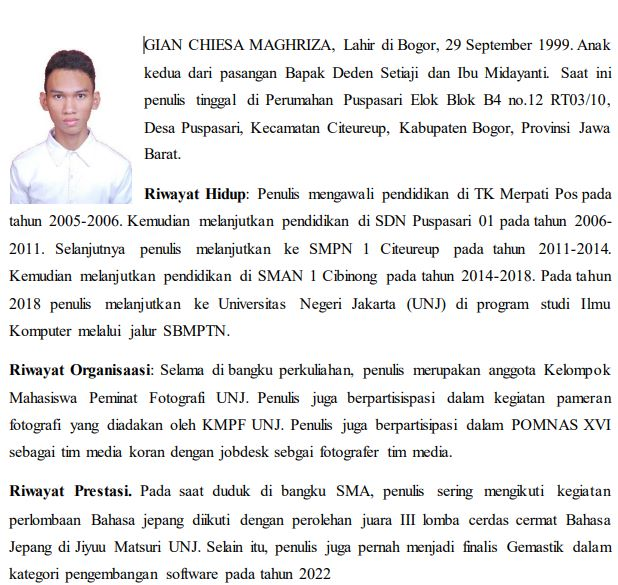
\includegraphics[keepaspectratio,width=0.96\textwidth, height=0.96\textheight]{gambar/riwayat}
\end{figure}
%-----------------------------------------------------------------
%Disini akhir masukan Daftar Pustaka
%-----------------------------------------------------------------


\end{document}